
%%%%%%%%%%%%%%%%%%%%%%%%%%%%%%%%%%%%%%%%%%%%%%%%%%%%%%%%%%%%%%%%%%%%%
%% This is a (brief) model paper using the achemso class
%% The document latex class accepts keyval options, which should include
%% the target journal and optionally the manuscript type.
%%%%%%%%%%%%%%%%%%%%%%%%%%%%%%%%%%%%%%%%%%%%%%%%%%%%%%%%%%%%%%%%%%%%%

% layout=traditional or twocolumn is other option
\documentclass[journal=jacsat,manuscript=article,layout=traditional]{achemso}
\setkeys{acs}{articletitle = true} % show titles in bibliography
%\documentclass[prb,11pt]{revtex4-1}
%\usepackage[sort&compress,numbers,super]{natbib} 
%\usepackage{achemso} 
\usepackage{wrapfig}
\usepackage{xargs}                      % Use more than one optional parameter in a new commands
\usepackage[pdftex,dvipsnames]{xcolor}  % Coloured text etc.
% 
\usepackage[colorinlistoftodos,prependcaption,textsize=tiny]{todonotes}
\newcommandx{\unsure}[2][1=]{\todo[linecolor=red,backgroundcolor=red!25,bordercolor=red,#1]{#2}}
\newcommandx{\change}[2][1=]{\todo[linecolor=OliveGreen,backgroundcolor=OliveGreen!25,bordercolor=OliveGreen,#1]{#2}}

\usepackage{amsfonts}
\usepackage{epigraph}

\usepackage[symbol]{footmisc}
\renewcommand{\thefootnote}{\fnsymbol{footnote}}

\setlength{\epigraphwidth}{0.7\textwidth}
%%%%%%%%%%%%%%%%%%%%%%%%%%%%%%%%%%%%%%%%%%%%%%%%%%%%%%%%%%%%%%%%%%%%%
%% Place any additional packages needed here.  Only include packages
%% which are essential, to avoid problems later. Do NOT use any
%% packages which require e-TeX (for example etoolbox): the e-TeX
%% extensions are not currently available on the ACS conversion
%% servers.
%%%%%%%%%%%%%%%%%%%%%%%%%%%%%%%%%%%%%%%%%%%%%%%%%%%%%%%%%%%%%%%%%%%%%
\usepackage[version=3]{mhchem} % Formula subscripts using \ce{}
\usepackage[T1]{fontenc}       % Use modern font encodings
\usepackage{subfig}
%\usepackage{hyperref}
\usepackage{xr} % external referecnes
\externaldocument{SI}
\newcommand{\angstrom}{\mbox{\normalfont\AA}}

\usepackage{natbib} 

%%%%%%%%%%%%%%%%%%%%%%%%%%%%%%%%%%%%%%%%%%%%%%%%%%%%%%%%%%%%%%%%%%%%%
%% If issues arise when submitting your manuscript, you may want to
%% un-comment the next line.  This provides information on the
%% version of every file you have used.
%%%%%%%%%%%%%%%%%%%%%%%%%%%%%%%%%%%%%%%%%%%%%%%%%%%%%%%%%%%%%%%%%%%%%
%%\listfiles

%%%%%%%%%%%%%%%%%%%%%%%%%%%%%%%%%%%%%%%%%%%%%%%%%%%%%%%%%%%%%%%%%%%%%
%% Place any additional macros here.  Please use \newcommand* where
%% possible, and avoid layout-changing macros (which are not used
%% when typesetting).
%%%%%%%%%%%%%%%%%%%%%%%%%%%%%%%%%%%%%%%%%%%%%%%%%%%%%%%%%%%%%%%%%%%%%
\newcommand*\mycommand[1]{\texttt{\emph{#1}}}

%%%%%%%%%%%%%%%%%%%%%%%%%%%%%%%%%%%%%%%%%%%%%%%%%%%%%%%%%%%%%%%%%%%%%
%% Meta-data block
%% ---------------
%% Each author should be given as a separate \author command.
%%
%% Corresponding authors should have an e-mail given after the author
%% name as an \email command. Phone and fax numbers can be given
%% using \phone and \fax, respectively; this information is optional.
%%
%% The affiliation of authors is given after the authors; each
%% \affiliation command applies to all preceding authors not already
%% assigned an affiliation.
%%
%% The affiliation takes an option argument for the short name.  This
%% will typically be something like "University of Somewhere".
%%
%% The \altaffiliation macro should be used for new address, etc.
%% On the other hand, \alsoaffiliation is used on a per author basis
%% when authors are associated with multiple institutions.
%%%%%%%%%%%%%%%%%%%%%%%%%%%%%%%%%%%%%%%%%%%%%%%%%%%%%%%%%%%%%%%%%%%%%
\author{Arni Sturluson}
\affiliation[Oregon State University]
{Oregon State University, School of Chemical, Biological, and Environmental Engineering. Corvallis, OR, USA.}
\author{Melanie T. Huynh}
\affiliation[Oregon State University]
{Oregon State University, School of Chemical, Biological, and Environmental Engineering. Corvallis, OR, USA.}
\author{Arthur H. P. York}
\affiliation[Oregon State University]
{Oregon State University, School of Chemical, Biological, and Environmental Engineering. Corvallis, OR, USA.}
\author{Cory M. Simon}
%\altaffiliation{A shared footnote}
\email{Cory.Simon@oregonstate.edu}
\affiliation[Oregon State University]
{Oregon State University, School of Chemical, Biological, and Environmental Engineering. Corvallis, OR, USA.}
%\altaffiliation{Current address: Some other place, Othert\"own,
%Germany}
%\author{I. Ken Groupleader}
%\altaffiliation{A shared footnote}
%\email{i.k.groupleader@unknown.uu}
%\phone{+123 (0)123 4445556}
%\fax{+123 (0)123 4445557}
%\affiliation[Unknown University]
%{Department of Chemistry, Unknown University, Unknown Town}
%\alsoaffiliation[Second University]
%{Department of Chemistry, Second University, Nearby Town}
%\author{Susanne K. Laborator}

%\affiliation[BigPharma]
%{Lead Discovery, BigPharma, Big Town, USA}
%\author{Kay T. Finally}



%%%%%%%%%%%%%%%%%%%%%%%%%%%%%%%%%%%%%%%%%%%%%%%%%%%%%%%%%%%%%%%%%%%%%
%% The document title should be given as usual. Some journals require
%% a running title from the author: this should be supplied as an
%% optional argument to \title.
%%%%%%%%%%%%%%%%%%%%%%%%%%%%%%%%%%%%%%%%%%%%%%%%%%%%%%%%%%%%%%%%%%%%%
\title[Latent space of porous cages]
  {Eigencages: Learning a latent space of porous cage molecules}

%%%%%%%%%%%%%%%%%%%%%%%%%%%%%%%%%%%%%%%%%%%%%%%%%%%%%%%%%%%%%%%%%%%%%
%% Some journals require a list of abbreviations or keywords to be
%% supplied. These should be set up here, and will be printed after
%% the title and author information, if needed.
%%%%%%%%%%%%%%%%%%%%%%%%%%%%%%%%%%%%%%%%%%%%%%%%%%%%%%%%%%%%%%%%%%%%%
\abbreviations{IR,NMR,UV}
\keywords{American Chemical Society, \LaTeX}

%%%%%%%%%%%%%%%%%%%%%%%%%%%%%%%%%%%%%%%%%%%%%%%%%%%%%%%%%%%%%%%%%%%%%
%% The manuscript does not need to include \maketitle, which is
%% executed automatically.
%%%%%%%%%%%%%%%%%%%%%%%%%%%%%%%%%%%%%%%%%%%%%%%%%%%%%%%%%%%%%%%%%%%%%
\begin{document}

%%%%%%%%%%%%%%%%%%%%%%%%%%%%%%%%%%%%%%%%%%%%%%%%%%%%%%%%%%%%%%%%%%%%%
%% The "tocentry" environment can be used to create an entry for the
%% graphical table of contents. It is given here as some journals
%% require that it is printed as part of the abstract page. It will
%% be automatically moved as appropriate.
%%%%%%%%%%%%%%%%%%%%%%%%%%%%%%%%%%%%%%%%%%%%%%%%%%%%%%%%%%%%%%%%%%%%%
\begin{tocentry}
%
%Some journals require a graphical entry for the Table of Contents.
%This should be laid out ``print ready'' so that the sizing of the
%text is correct.
%
%Inside the \texttt{tocentry} environment, the font used is Helvetica
%8\,pt, as required by \emph{Journal of the American Chemical
%Society}.
%
%The surrounding frame is 9\,cm by 3.5\,cm, which is the maximum
%permitted for  \emph{Journal of the American Chemical Society}
%graphical table of content entries. The box will not resize if the
%content is too big: instead it will overflow the edge of the box.
%
%This box and the associated title will always be printed on a
%separate page at the end of the document.
%
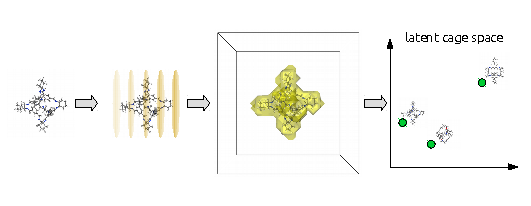
\includegraphics[width=9cm]{../toc_graphic.pdf}
\end{tocentry}

%%%%%%%%%%%%%%%%%%%%%%%%%%%%%%%%%%%%%%%%%%%%%%%%%%%%%%%%%%%%%%%%%%%%%
%% The abstract environment will automatically gobble the contents
%% if an abstract is not used by the target journal.
%%%%%%%%%%%%%%%%%%%%%%%%%%%%%%%%%%%%%%%%%%%%%%%%%%%%%%%%%%%%%%%%%%%%%
\begin{abstract}
Porous organic cage molecules harbor nano-sized cavities that can selectively adsorb gas molecules, lending them applications in separations and sensing. The geometry of the cavity strongly influences their adsorptive selectivity.
For comparing cages and predicting their adsorption properties, we embed/encode a set of 74 porous organic cage molecules into a low-dimensional, latent ``cage space'' on the basis of their intrinsic porosity.
We first computationally scan each cage to generate a 3D image of its porosity. 
Leveraging the singular value decomposition, in an unsupervised manner, we then learn across all cages an approximate, lower-dimensional subspace in which the {\color{red} 3D porosity images} lay.
The ``eigencages'' are the set of orthogonal characteristic {\color{red} 3D porosity images} that span this lower-dimensional subspace, ordered in terms of importance. A latent representation/encoding of each cage follows from expressing it as a combination of the eigencages. 
We show that the learned encoding captures salient features of the cavities of porous cages and is predictive of properties of the cages that arise from cavity shape.
\end{abstract}

%%%%%%%%%%%%%%%%%%%%%%%%%%%%%%%%%%%%%%%%%%%%%%%%%%%%%%%%%%%%%%%%%%%%%
%% Start the main part of the manuscript here.
%%%%%%%%%%%%%%%%%%%%%%%%%%%%%%%%%%%%%%%%%%%%%%%%%%%%%%%%%%%%%%%%%%%%%
\section{Introduction}
More than 10\% of the world's energy consumption is devoted to purifying chemical mixtures \cite{sholl2016seven}. The development of more energy-efficient processes to separate mixtures thus would significantly reduce carbon emissions and the cost of manufacturing goods. Gaseous mixtures in particular could be separated more energy-efficiently than by e.g.\ distillation \cite{doe_study} instead via selective adsorption on a solid-state, porous material\footnote[2]{The energy requirement for separating a mixture has a thermodynamic limit \cite{bhown2011analysis}, of course.}. Porous solids composed of porous organic cage molecules \cite{tozawa2009porous} have auspiciously demonstrated the ability to separate gases \cite{hasell2016porous} in application to carbon dioxide capture from natural gas \cite{mastalerz2011salicylbisimine} and flue gas of coal-fired power plants \cite{tian2009amorphous,hong2015porphyrin}, xenon/krypton separations \cite{chen2014separation,patil2016noria}, and sulfur hexaflouride capture \cite{sf6seps}. Porous cage solids with high adsorptive selectivities may serve as vapor sensors as well \cite{brutschy2012porous,brutschy2013direct}.

Porous organic cages \cite{hasell2016porous,holst2010porous,cooper2017porousacs} are molecules that harbor (i) a cavity that is intrinsic to their molecular structure and (ii) windows through which gas molecules can enter the cavity. Often, the cavity is large enough to accommodate only a single small gas molecule \cite{miklitz2017computational}. Unlike metal- \cite{furukawa2013chemistry} and covalent- \cite{diercks2017atom} organic frameworks, which are extended networks of molecular building blocks held together by directional coordination and covalent bonds, respectively, the assembly/packing of porous organic cage molecules to form a bulk porous cage solid is dictated by the geometry of the molecules and non-covalent/non-coordination interactions between them\cite{mckeown2010nanoporous}. 
%Thus, in addition to the intrinsic porosity of the cage molecule, extrinsic porosity can arise from the manner in which the cage molecules pack together to form the bulk solid.
%This discrete molecular nature of porous cage solids offers advantages over extended network materials \cite{holst2010porous} in facile post-synthetic functionalization using solution chemistry \cite{schneider2013post}, mixing of different functionalities\unsure{citation for this. also mention MTV MOFs}, and inducing dramatic changes in properties induced by external factors via the interconversion of different polymorphs, e.g. on-off porosity \cite{jones2011off}\unsure{though this is possible for mofs too}. 
On the order of hundreds of porous organic cages have been reported \cite{evans2016computational}.

For deployment in molecular separations or vapor sensing, the size and shape of the cavities in a porous material can strongly influence the adsorptive selectivity \cite{mitra2013molecular,zhu1999shape,lee2018high,smit2008towards,sikora2012thermodynamic}. In a shape-selective molecular separation, the shape of the cavity or window in a porous material is such that it accommodates a subset of molecular species but excludes the remaining species through steric hindrance \cite{smit2008towards}. Aside from geometric exclusion, the size and shape of the cavity influence the enthalpy of adsorption, e.g. by encompassing the adsorbed gas molecule with chemical moieties in close proximity with which to interact \cite{simon2015best}, and the entropy of adsorption, e.g. by minimizing the loss of rotational entropy in the cavity \cite{denayer2005rotational}. Therefore, it is important to mathematically characterize the geometry of the cavity/void space in nanoporous materials for predicting adsorption and comparing materials. Several methods to mathematically describe pores of materials include using the Voronoi decomposition \cite{pinheiro2013characterization,martin2011addressing}, algebraic topology \cite{lee2017quantifying}, radial distribution functions \cite{fernandez2013atomic}, and density of minima in the potential energy landscape \cite{oganov2009quantify}. For extended networks, the MOFomics \cite{first2013mofomics} approach fits cylinders to the channels and describes the pore landscape as a graph of spheres (representing cages) connected to cylinders. Simple descriptors of cavities in porous cages such as the void and window diameters can be computed with \texttt{pywindow} \cite{miklitz2018pywindow}.

In this work, our goal is to map porous organic cage molecules to a lower-dimensional latent space\footnote{{\color{red} `Latent' space refers to `hidden' space: abstractly, it is a lower-dimensional subspace/manifold--which is embedded in data space-- in/on which the data congregates.}} on the basis of their intrinsic porosity. i.e., we aim to develop an information-rich, low-dimensional vector representation-- a fingerprint-- of each porous organic cage that encodes the salient features of the size and shape of its cavity and windows. Such a fingerprint is useful for a few reasons. First, the latent representation would serve as a predictor of adsorption in a regression or classification model as in Refs. \cite{bucior2018energy,simon2015best}; see Le et al.~\cite{le2012quantitative} for a review on quantitative structure-property modeling. Second, the latent representation lends a notion of similarity between two cages. Suppose a highly shape-selective porous cage molecule is composed of expensive or toxic precursors or suffers from instability. Within the latent cage space, we can then identify its nearest neighbors for alternative, existing cage molecules possessing the most similar cavity shapes, but composed of cheaper/safer precursors and showing higher stability. Finally, embedding porous cage molecules into a low-dimensional latent space and analyzing the clusters can shed light on the diversity of  cavity shapes among the cages that have been synthesized.

Herein, we automatically learn a latent representation of the cavities of porous cages from a training dataset of 74 porous organic cage molecules \cite{miklitz2017computational,greenaway2018high}. We achieve this by first computationally scanning the cage molecules to generate 3D images of their porosity, {\color{red} with the cavity in the center of the image}. The pixels in the image represent a point in space and the binary pixel values represent whether the space is void or occupied by a cage atom.
We postulate that these 3D porosity images, which belong to an enormous space, approximately lay in a much lower-dimensional subspace. Inspired by eigenfaces in facial recognition \cite{sirovich1987low,turk1991face,muller2004singular}, we then employ the singular value decomposition to, in an unsupervised manner, identify a set of characteristic 3D porosity images-- \emph{eigencages}-- that form an orthonormal basis for this approximate, lower-dimensional subspace in which the 3D porosity images lay. A low-dimensional \emph{latent representation} follows by expressing each cage as a combination of the eigencages. {\color{red} Visualizing a 2D embedding of our \emph{latent cage space} with t-SNE \cite{maaten2008visualizing}} shows that the learned encoding captures salient features of the cavities of porous cages and is predictive of simulated xenon/krypton selectivity {\color{red} in isolated cage molecules}.


% We first describe our raw representation of the cavities of the cages, a three-dimensional scan of the porosity; in the resulting 3D images, pixels represent a point in space and the binary pixel values represent whether the space is void or occupied by a cage atom.

% We achieve this by first scanning the cavities of 74 porous organic cage molecules \cite{miklitz2017computational,greenaway2018high} to generate 3D images of their porosity. The pixels in the image represent a point in space and the binary pixel values represent whether the space is void or occupied by a cage atom.
%Our postulate is that these 3D cage cavity images, which belong to an enormous space, approximately lay in a much lower-dimensional subspace. We employ the singular value decomposition \cite{muller2004singular,kalman1996singularly,strang1993introduction} to learn the latent space of cage cavities in an unsupervised manner.



%We first describe our raw representation of the cavities of the cages, a three-dimensional scan of the porosity; in the resulting 3D images, pixels represent a point in space and the binary pixel values represent whether the space is void or occupied by a cage atom. We postulate that these 3D cage cavity images, which belong to an enormous space, approximately lay in a much lower-dimensional subspace. Inspired by eigenfaces in facial recognition \cite{sirovich1987low,turk1991face,muller2004singular}, we then employ the singular value decomposition to, in an unsupervised manner, identify a set of characteristic 3D void space images-- \emph{eigencages}-- that form an orthonormal basis for this approximate, lower-dimensional subspace in which the 3D void space images lay. Expressing each cage as a combination of the eigencages lends a low-dimensional \emph{latent representation} of the cages. By embedding the low-dimensional latent representations into a 2D \emph{latent cage space} for visualization, we show that the learned encoding captures salient features of the cavities of porous cages and is predictive of simulated xenon/krypton selectivity.

\section{The porous organic cage molecule dataset} Our training data set consists of the identity and spatial coordinates of the atoms comprising 74 porous organic cage molecules. A subset, 41 cages, were compiled by Miklitz et al. \cite{miklitz2017computational}, {\color{red} who extracted cage molecules from crystal structures determined by X-ray diffraction studies and deposited in the Cambridge Structural Database \cite{allen2002cambridge} by various research groups \cite{hasell2016porous,evans2015synthesis,zhang2014organic}}. The remaining cages are from a recent study that employed robots and {\color{red} computational predictions of cage topologies} \cite{greenaway2018high} to synthesize 33 different cages. {\color{red} The atomic coordinates of the latter set of cage structures were obtained by molecular modeling, a subset of which were confirmed by X-ray diffraction studies \cite{greenaway2018high}.} Fig.~\ref{fig:cages} illustrates the diversity of cage structures comprising the data set; Fig.~\ref{fig:allcagesdetailed} shows larger images of each cage. The spread of cavity and molecule diameters among the cages is shown in Fig.~\ref{fig:pywindow_descriptors_distn}.

\begin{figure}
\centering
	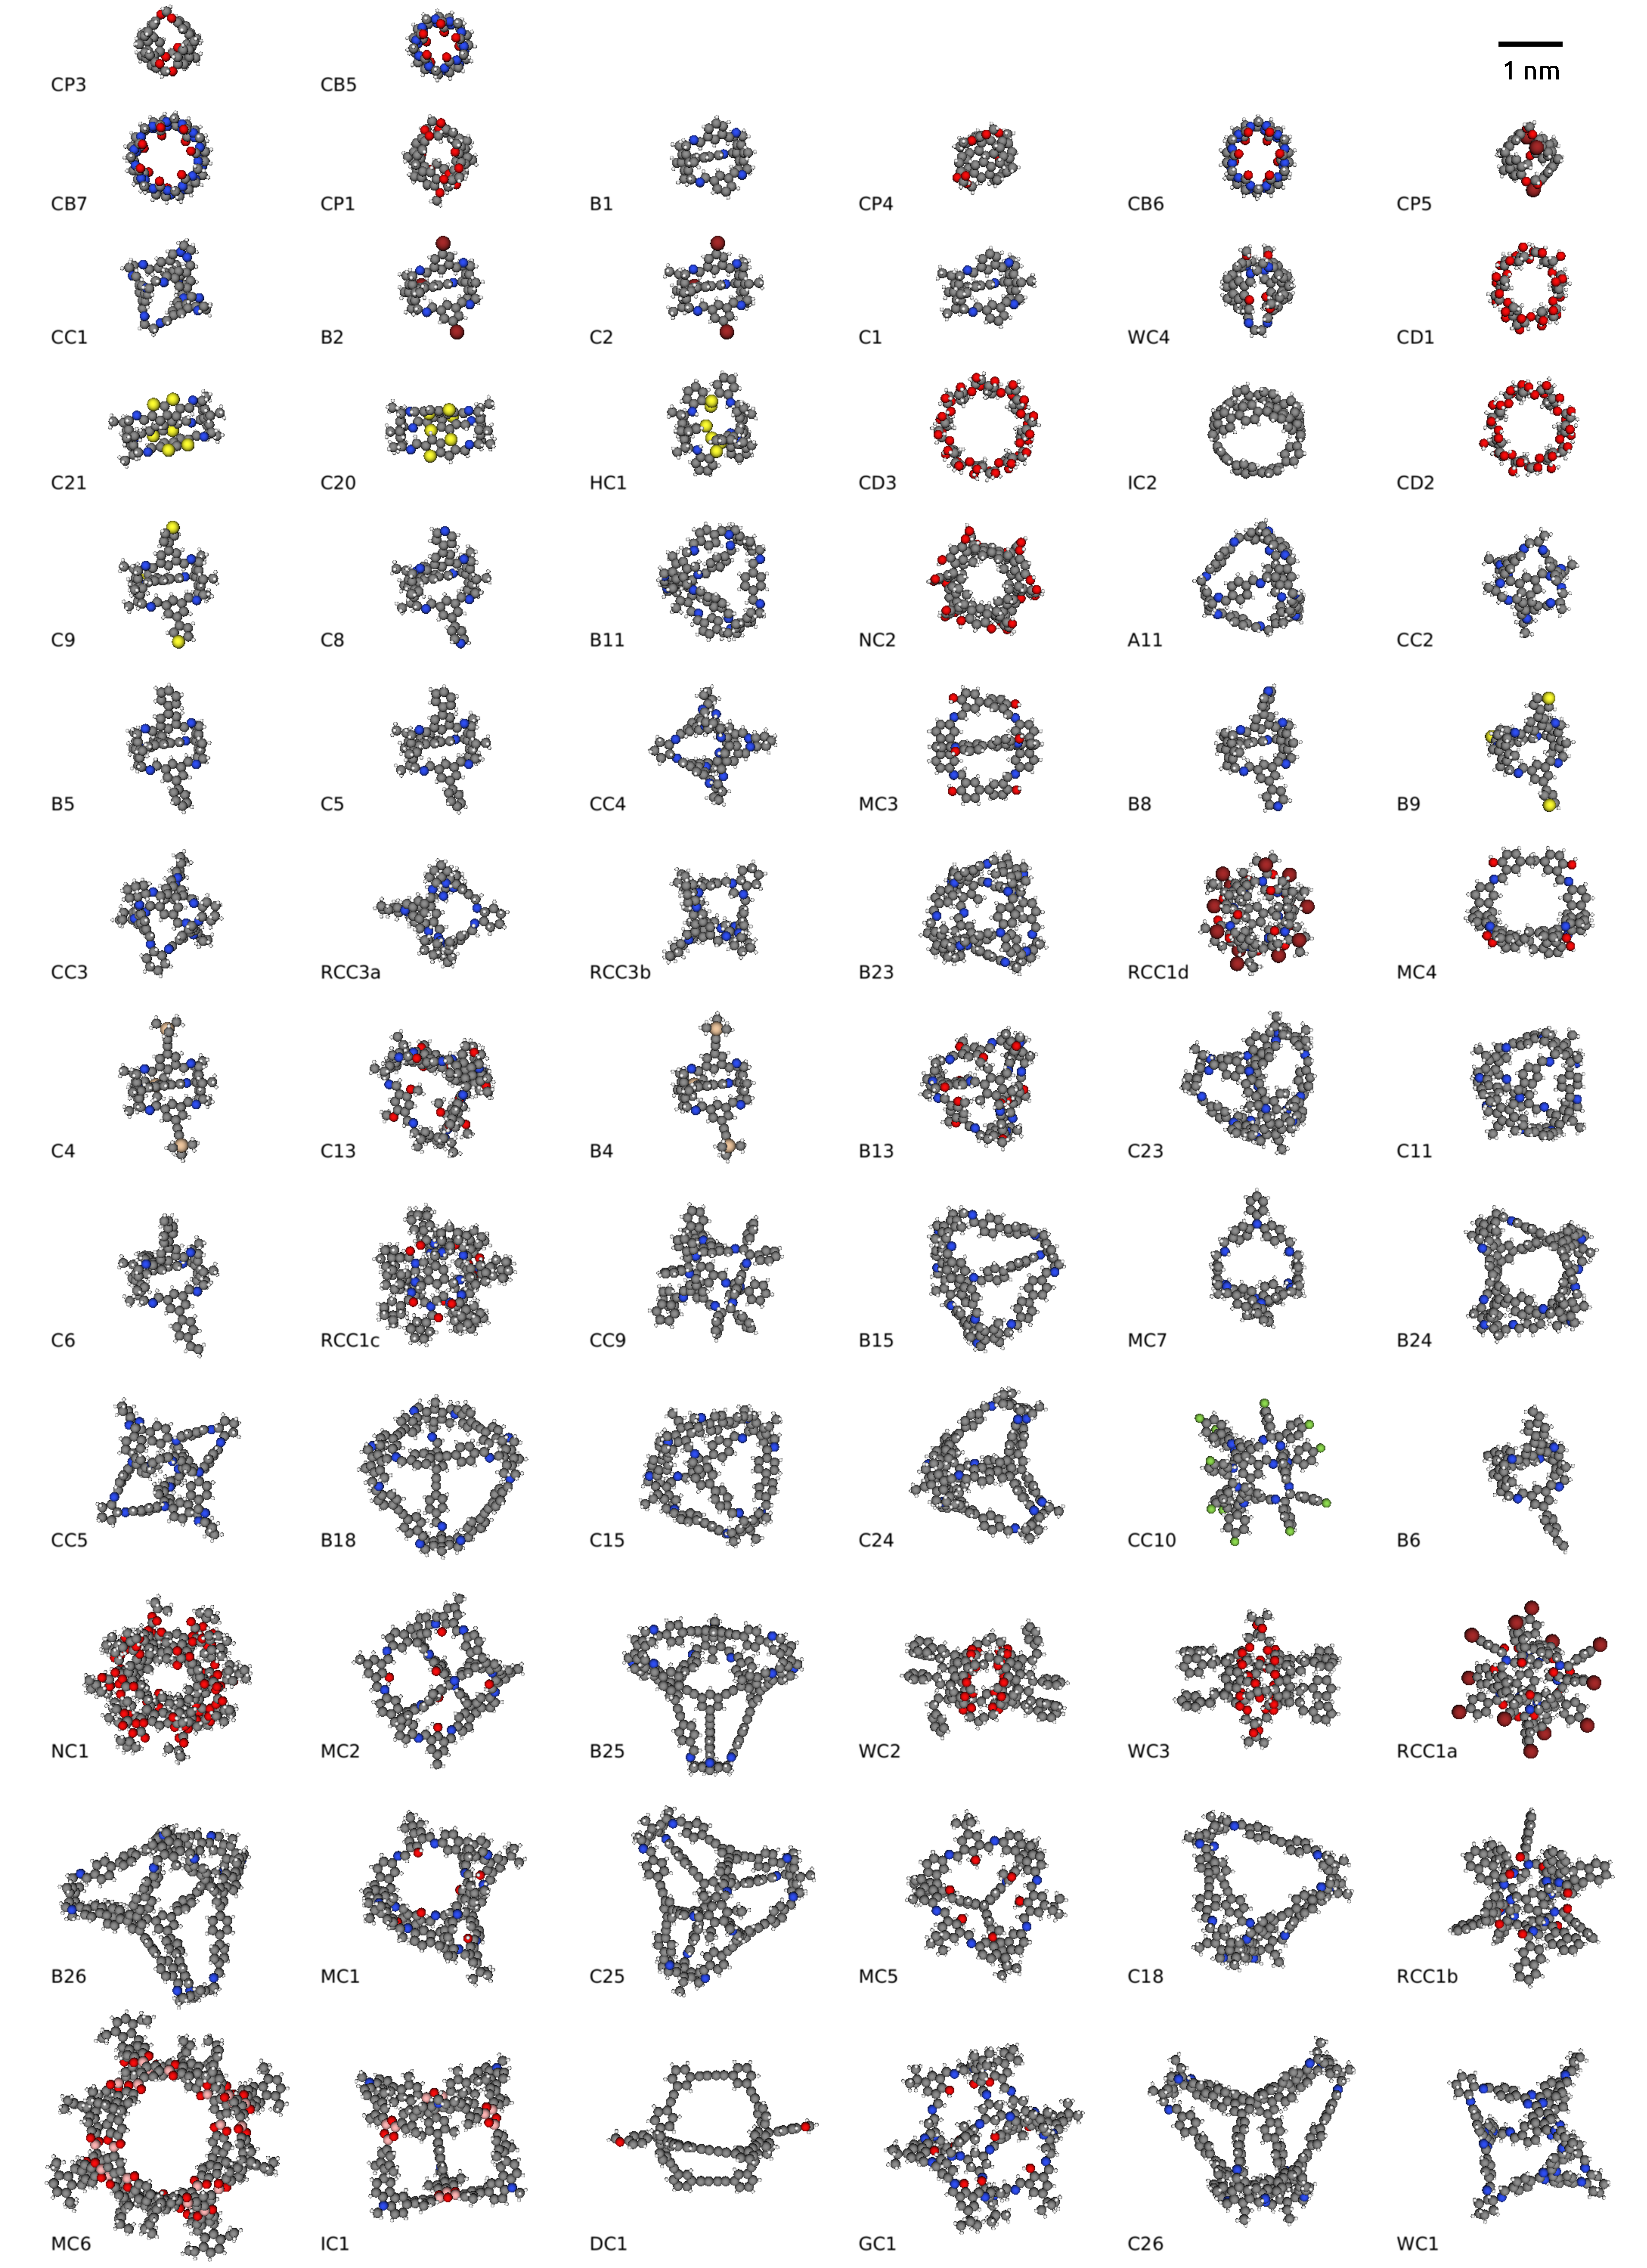
\includegraphics[width=0.9\columnwidth]{../final_aligned_cages/grid_of_cages_labeled.pdf} % from GIMP
	\caption{The structures of all {\color{red} aligned} 74 porous organic cage molecules \cite{miklitz2017computational,greenaway2018high} comprising the training set in this study, ordered by cage molecule diameter computed from \texttt{pywindow} \cite{miklitz2018pywindow}. Note the diversity of cavities.
	} \label{fig:cages}
\end{figure}

\section{Scanning the cages to generate 3D images of their porosity} We describe here how we generate a raw 3D image of the porosity of a cage. These images can be conceptualized as a computerized tomography (CT) scan of a porous organic cage molecule. Fig.~\ref{fig:raw3Dimages} depicts example raw 3D porosity images.

\begin{figure}
% made with image zoom 1.4. see saved VisIT session in data/grids. mesh width 4, see snapshot.vtk
\centering
	\subfloat[][\textbf{B15} \cite{greenaway2018high}]{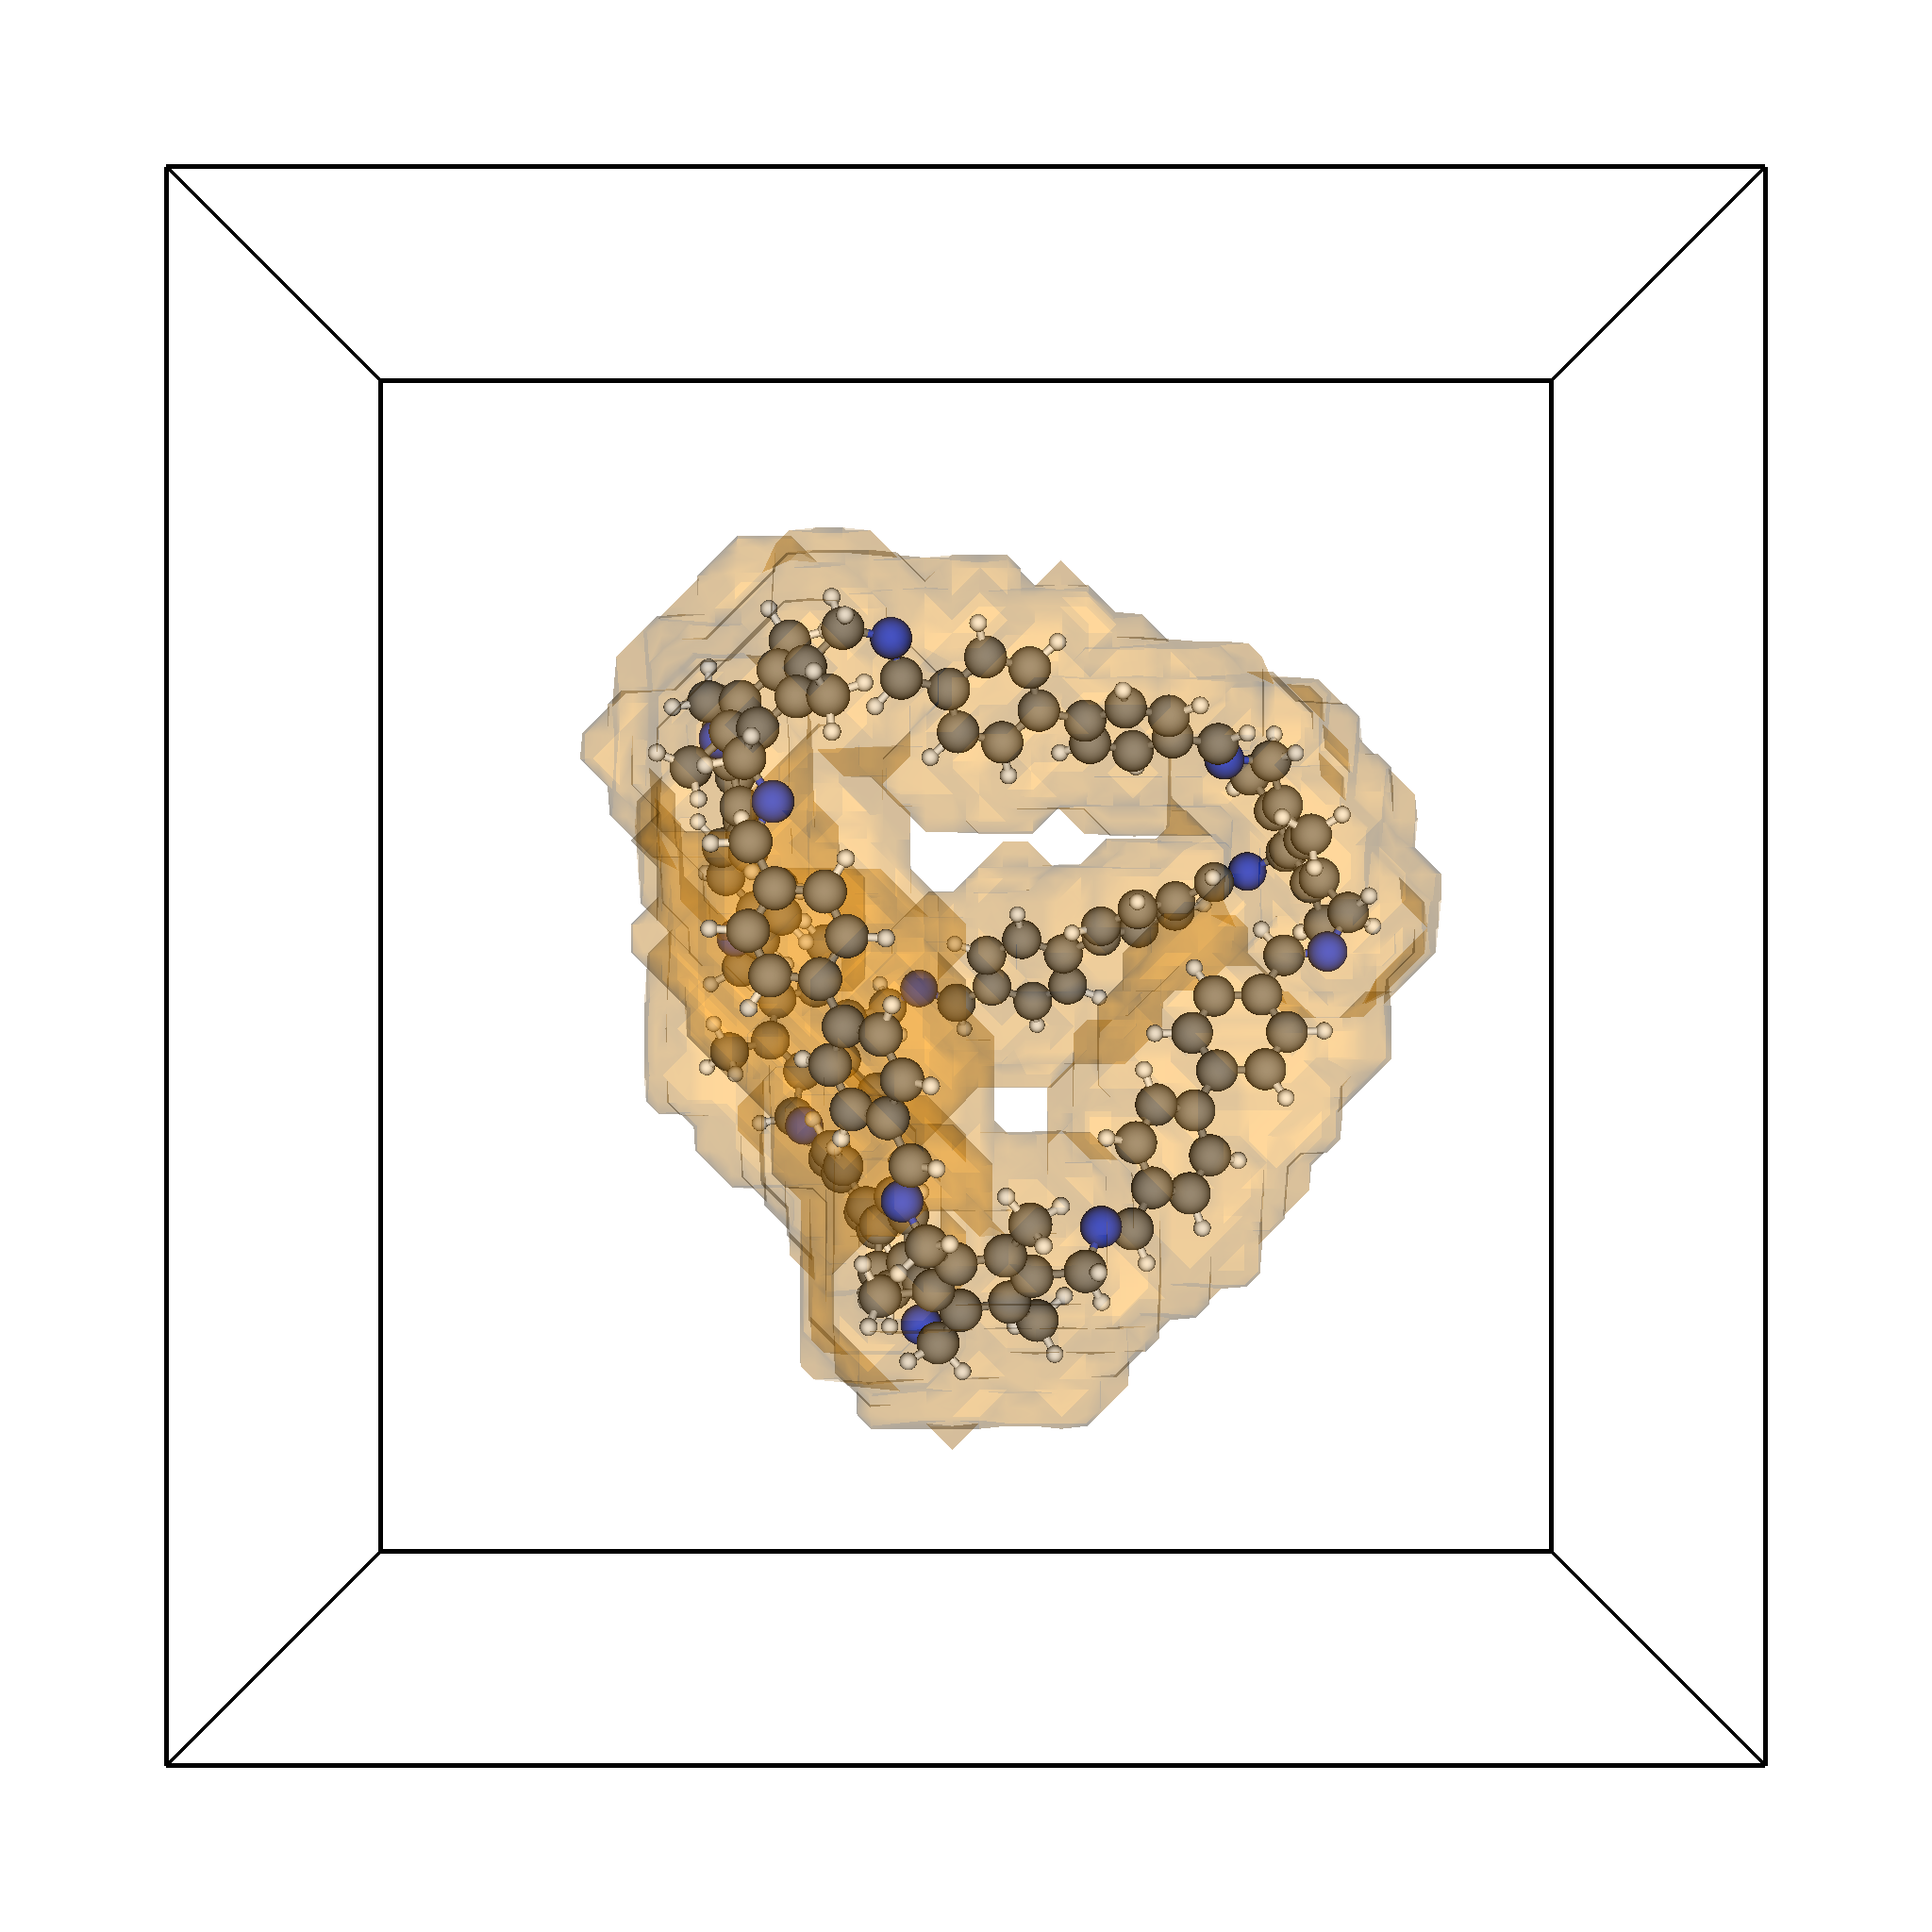
\includegraphics[width=0.3\columnwidth]{B15_raw.png}}
	\subfloat[][\textbf{B24} \cite{greenaway2018high}]{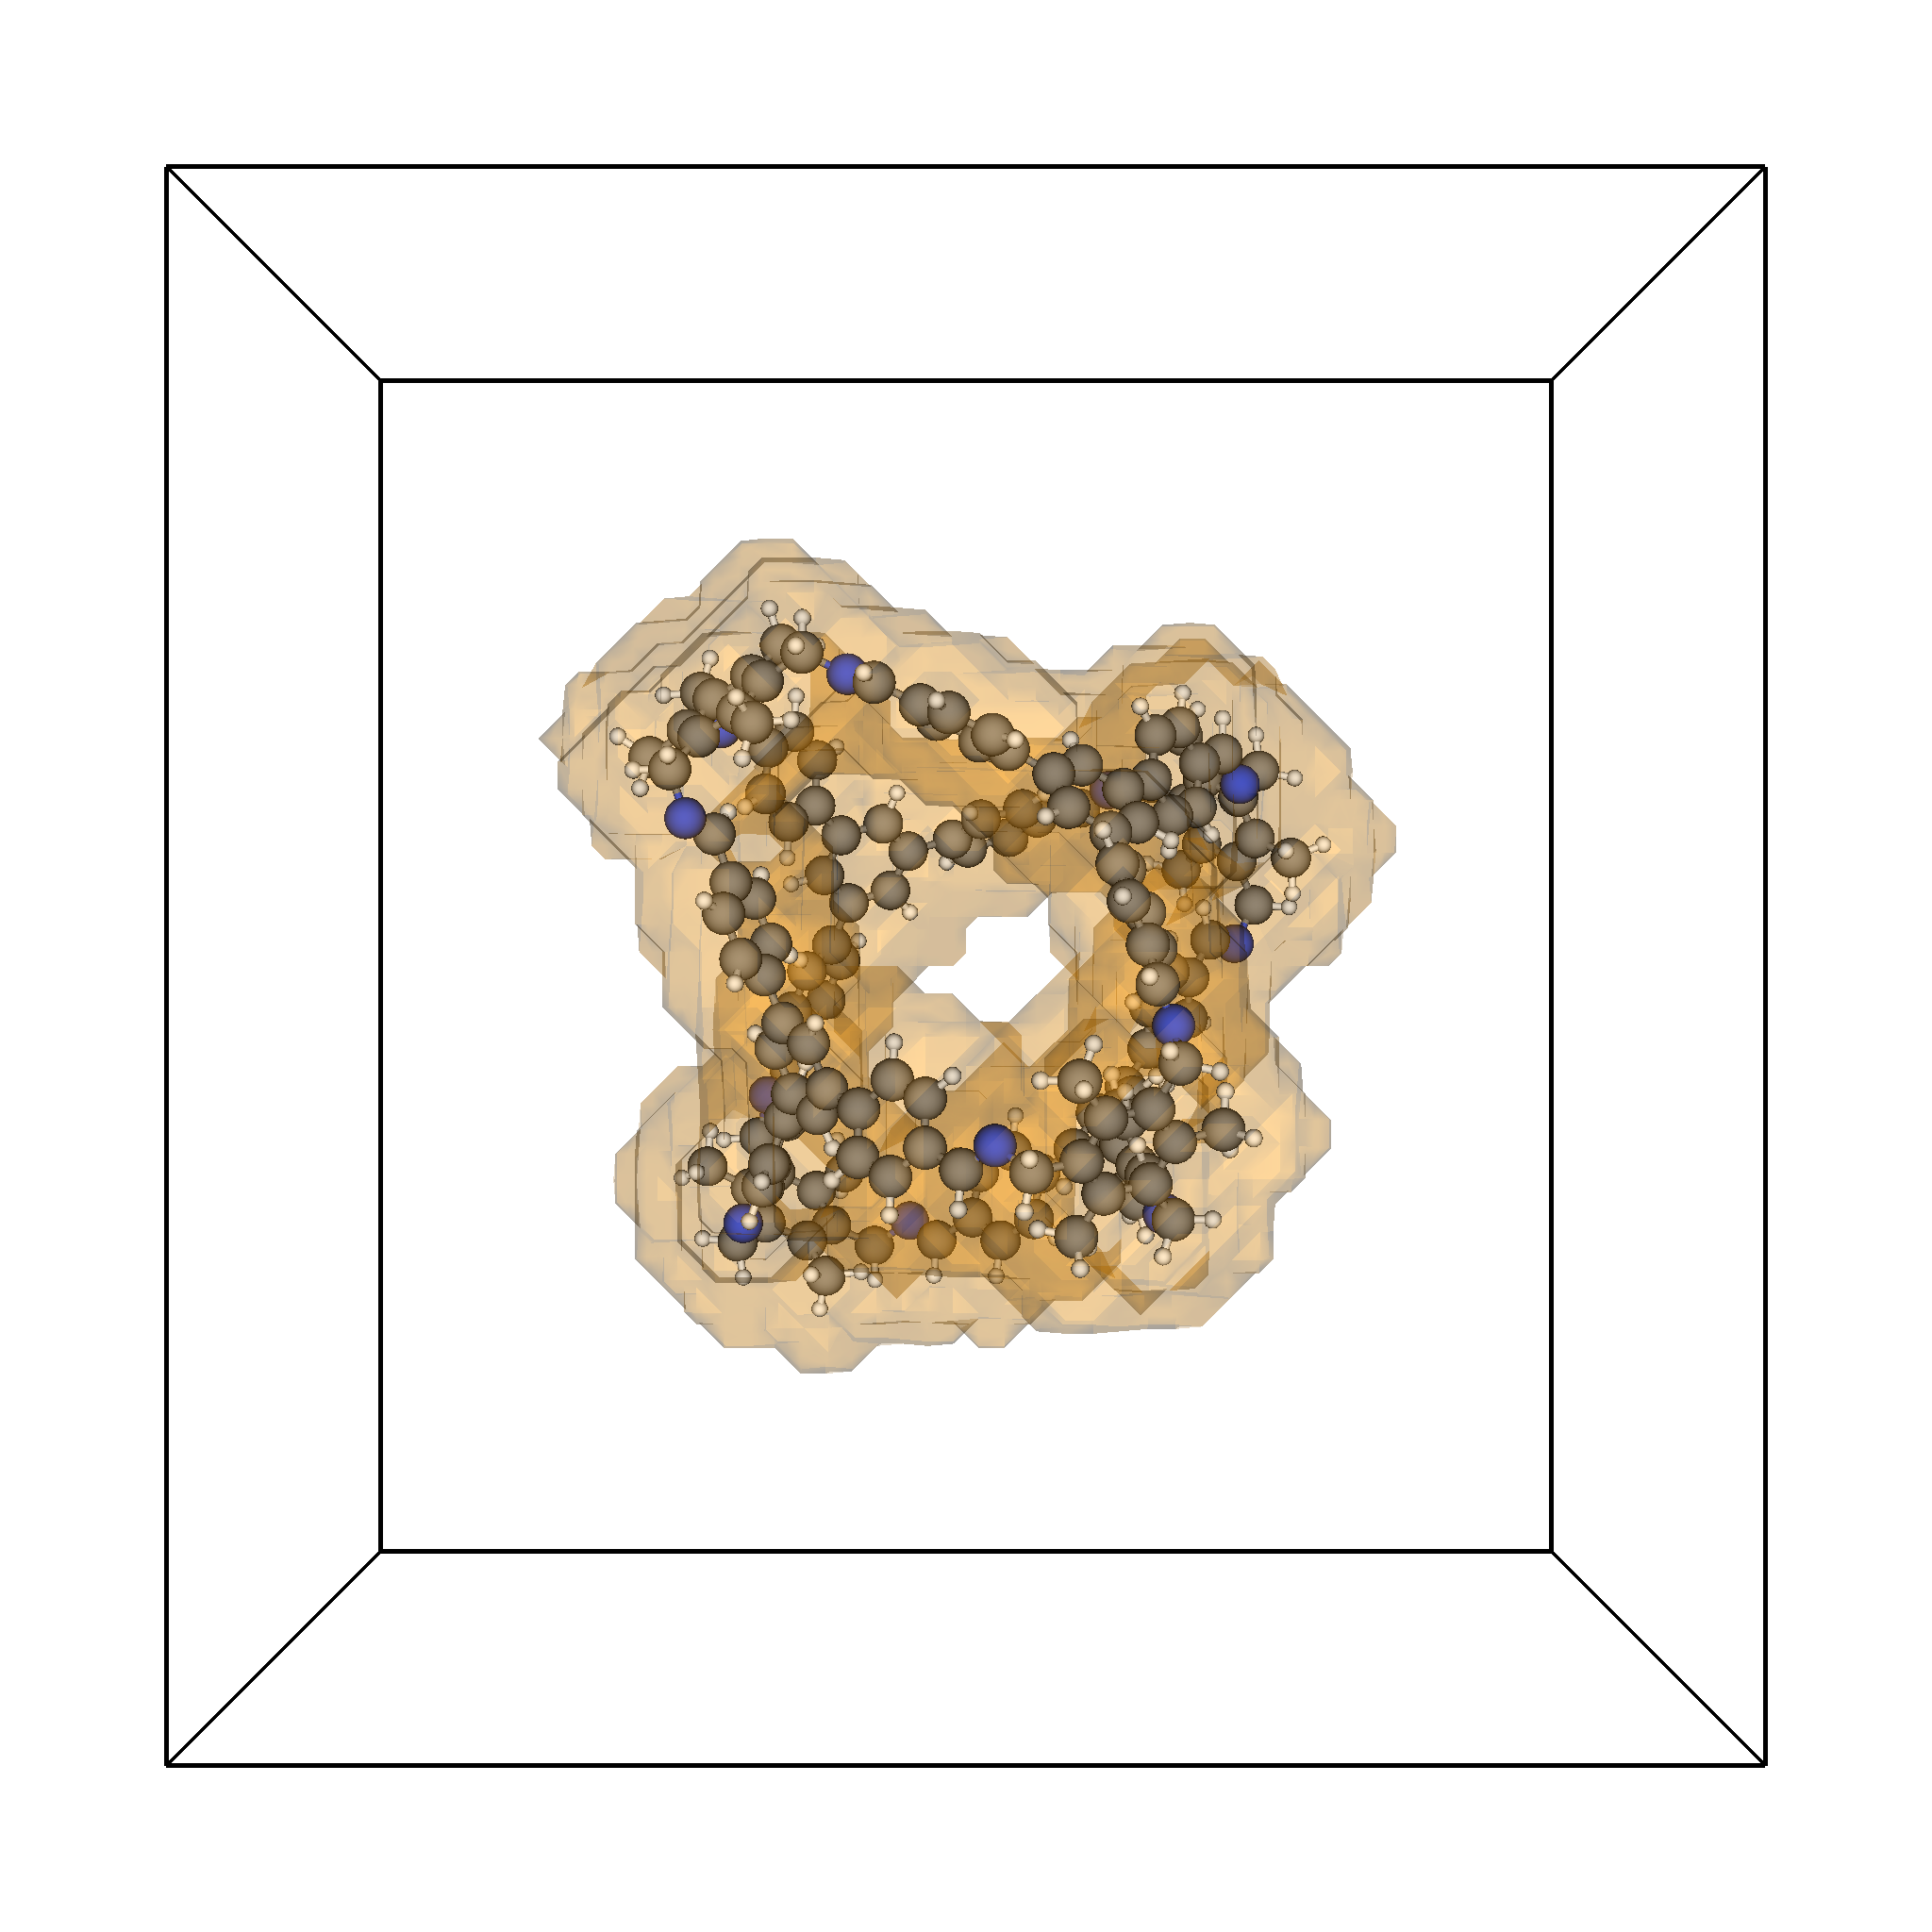
\includegraphics[width=0.3\columnwidth]{B24_raw.png}}
	\qquad
	\subfloat[][\textbf{C6} \cite{greenaway2018high}]{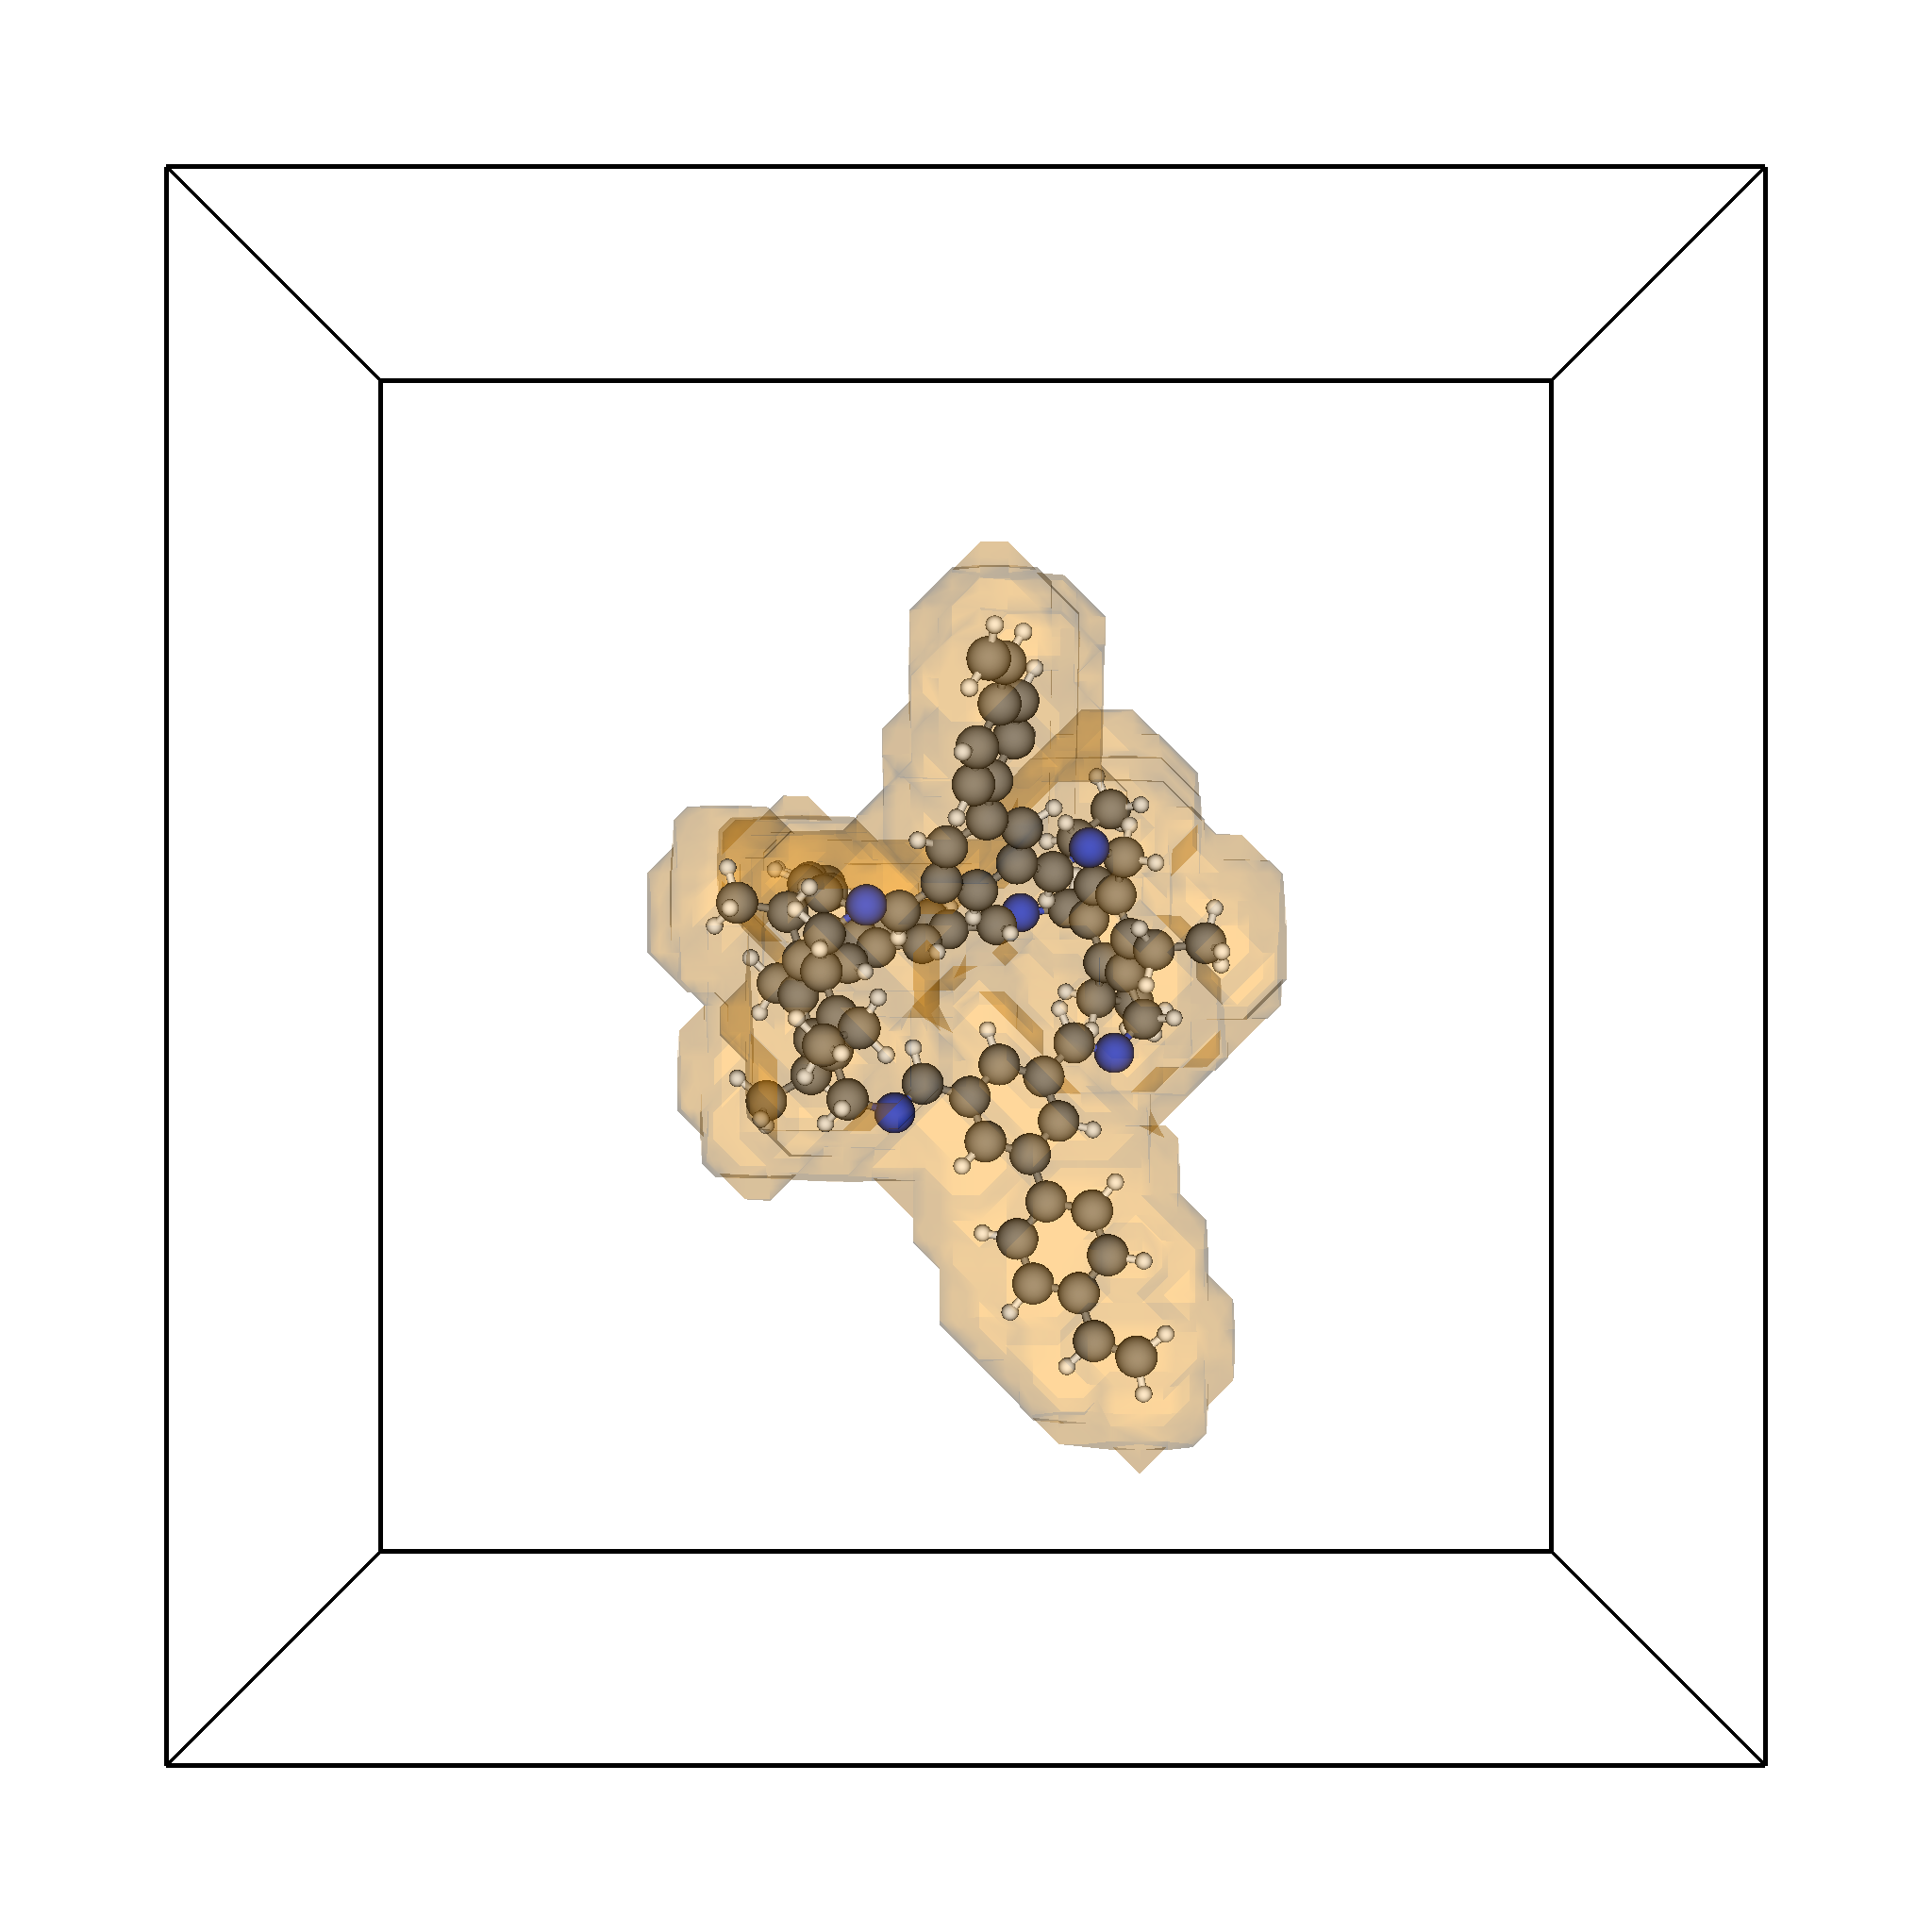
\includegraphics[width=0.3\columnwidth]{C6_raw.png}}
	\subfloat[][\textbf{CD2} \cite{crini2014history}]{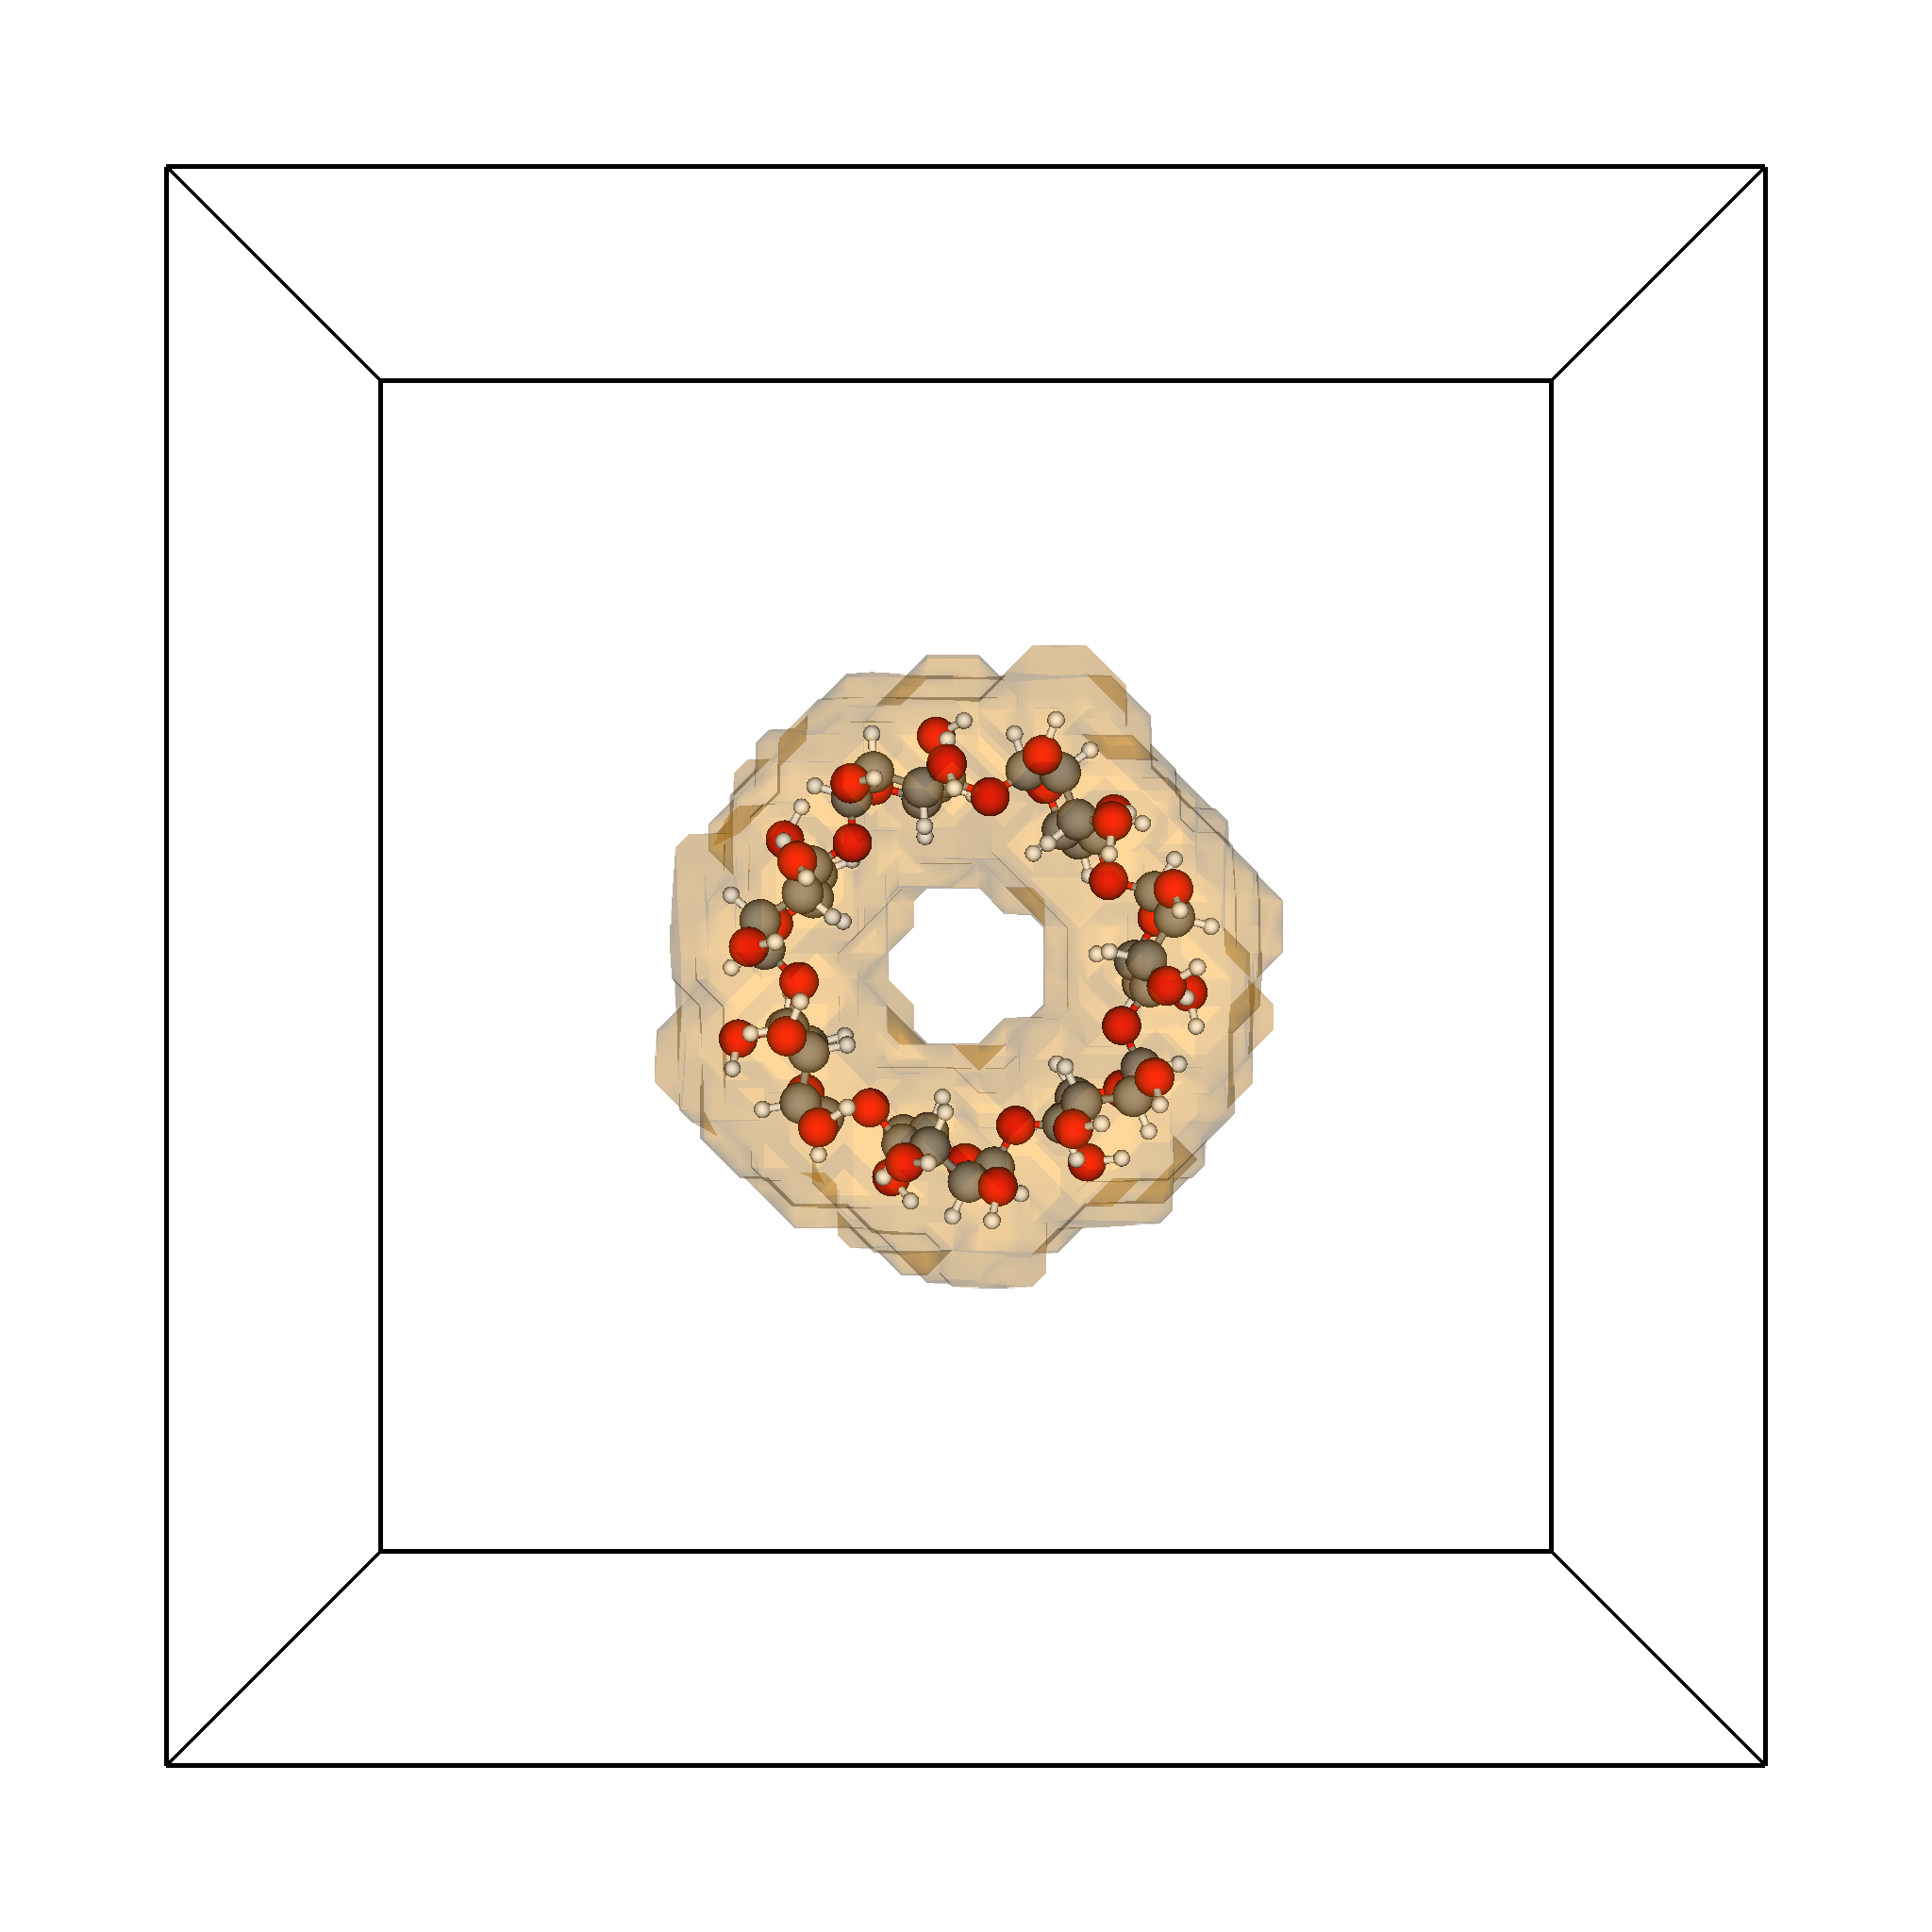
\includegraphics[width=0.3\columnwidth]{CD2_raw.png}}
	\qquad
	\subfloat[][\textbf{HC1} \cite{horng2009preparation}]{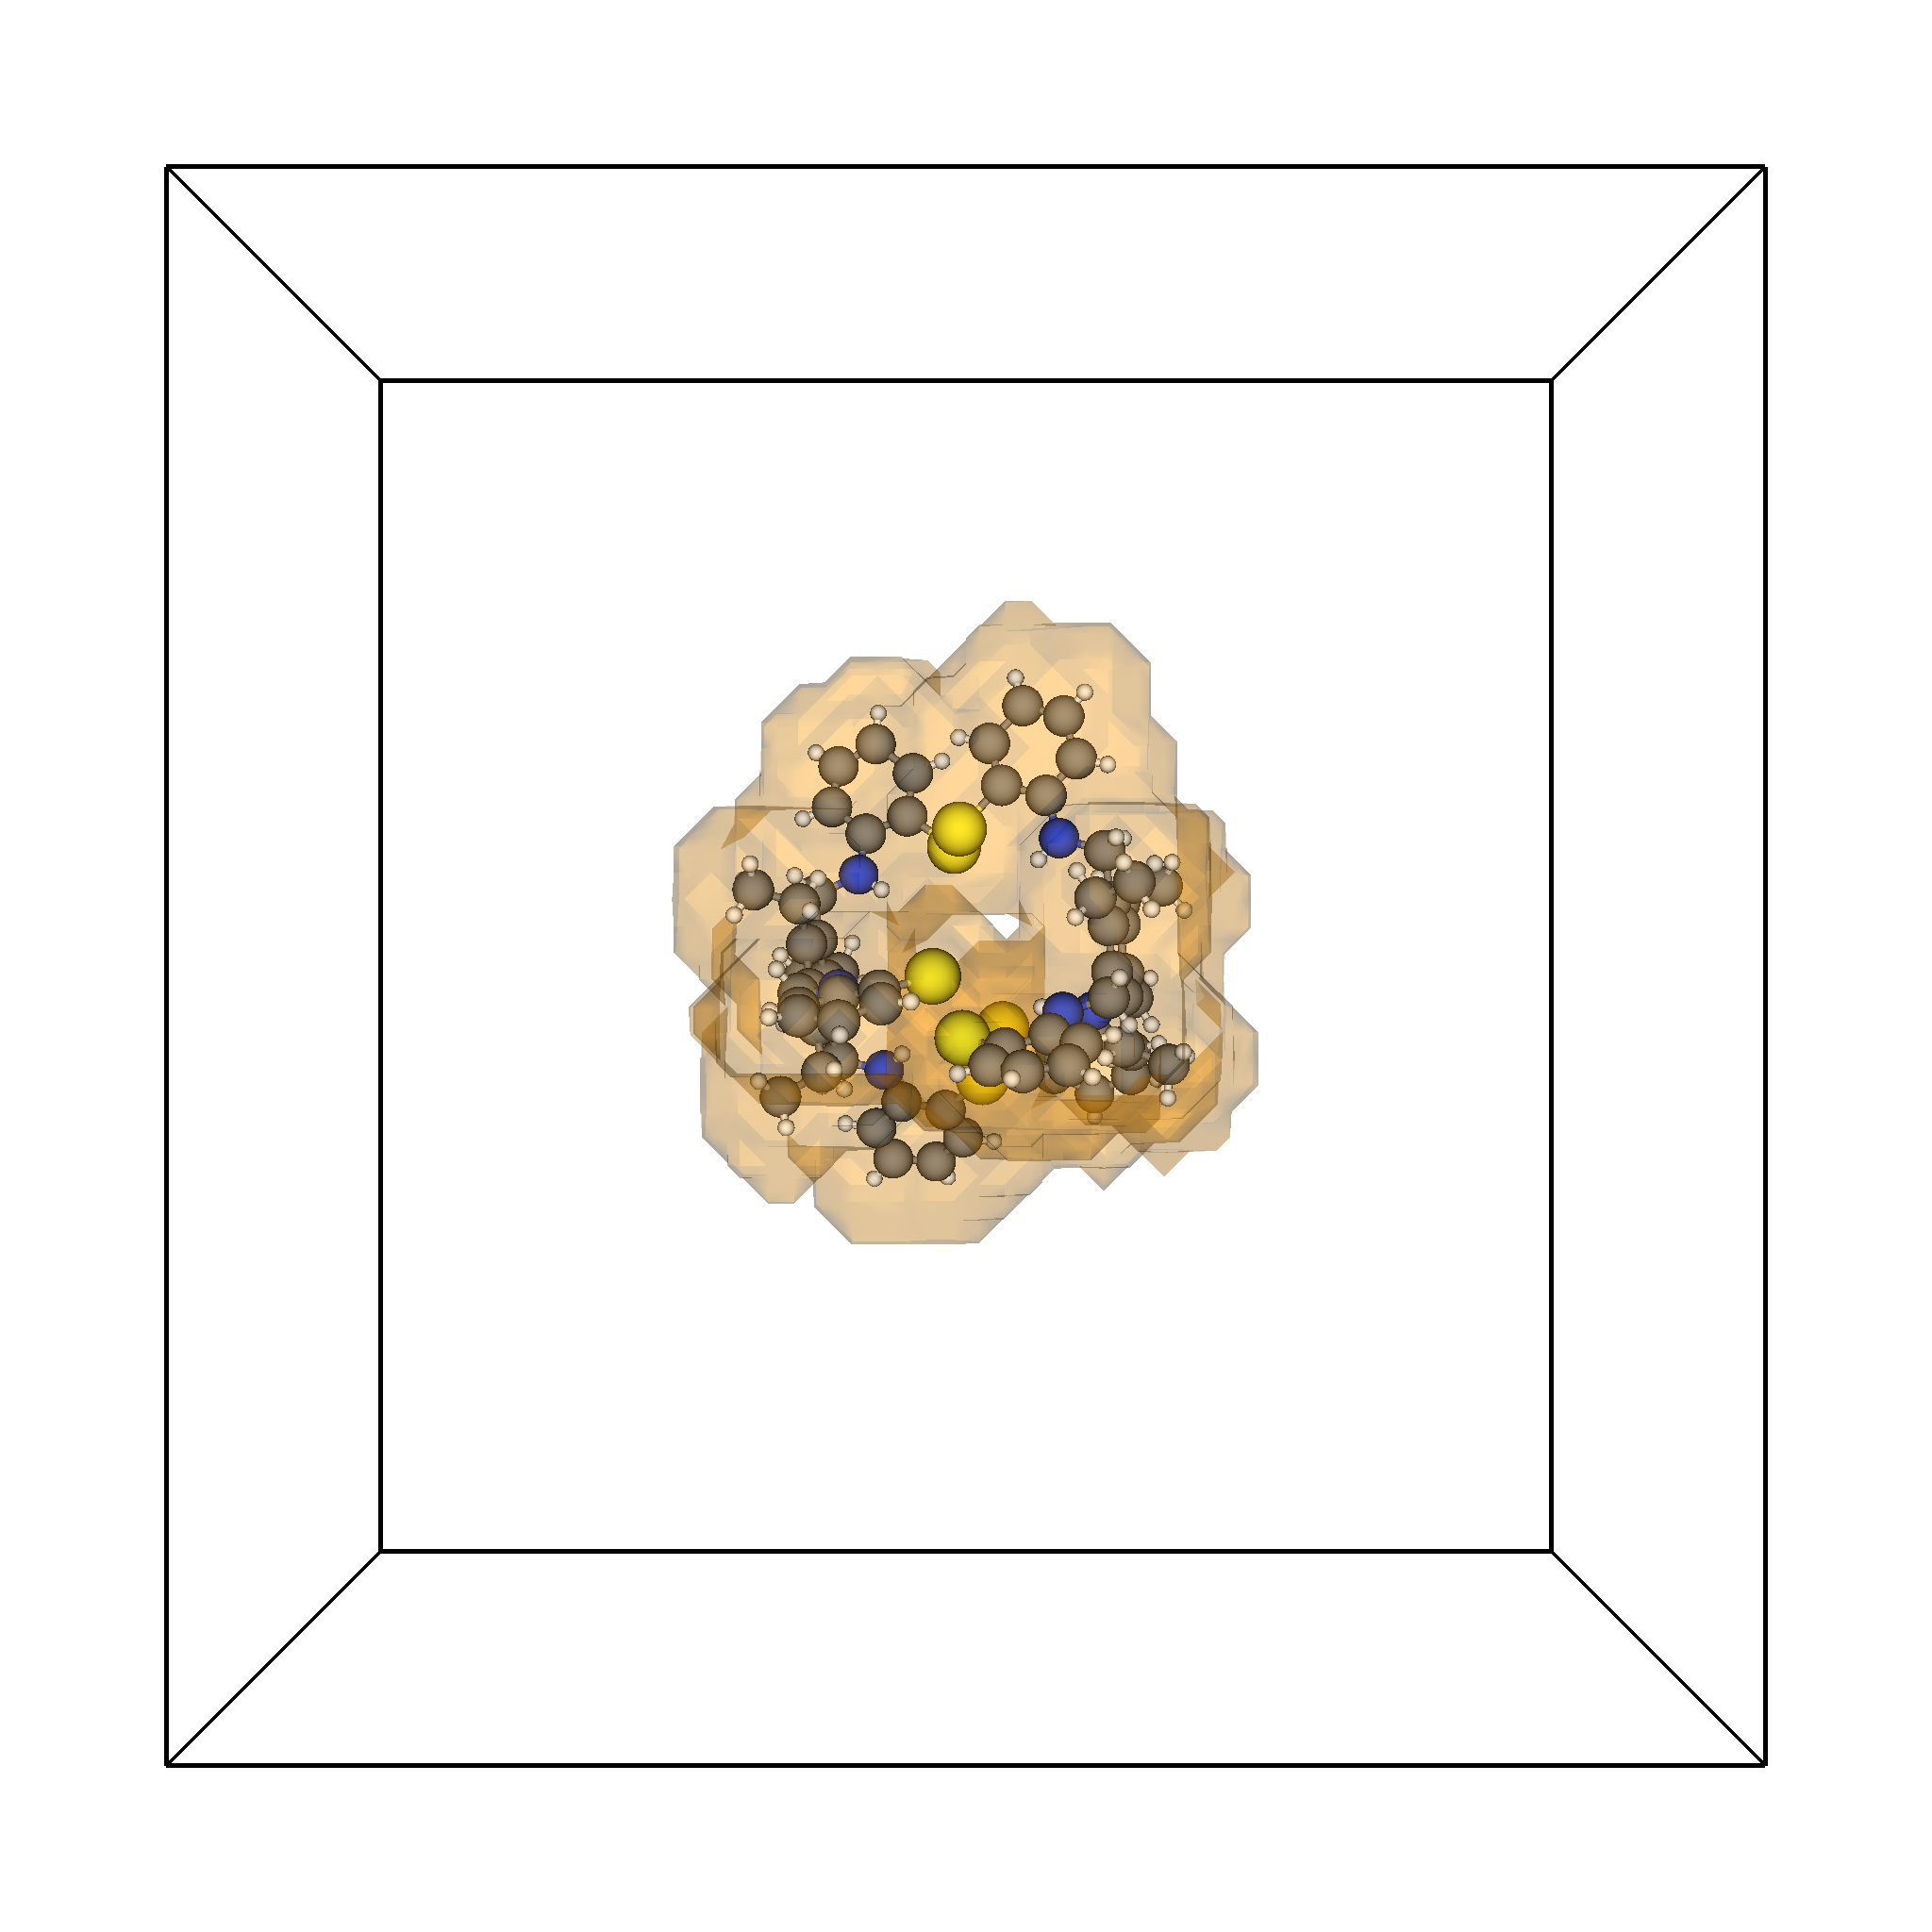
\includegraphics[width=0.3\columnwidth]{HC1_raw.png}}
	\subfloat[][\textbf{WC1} \cite{ding2015targeted}]{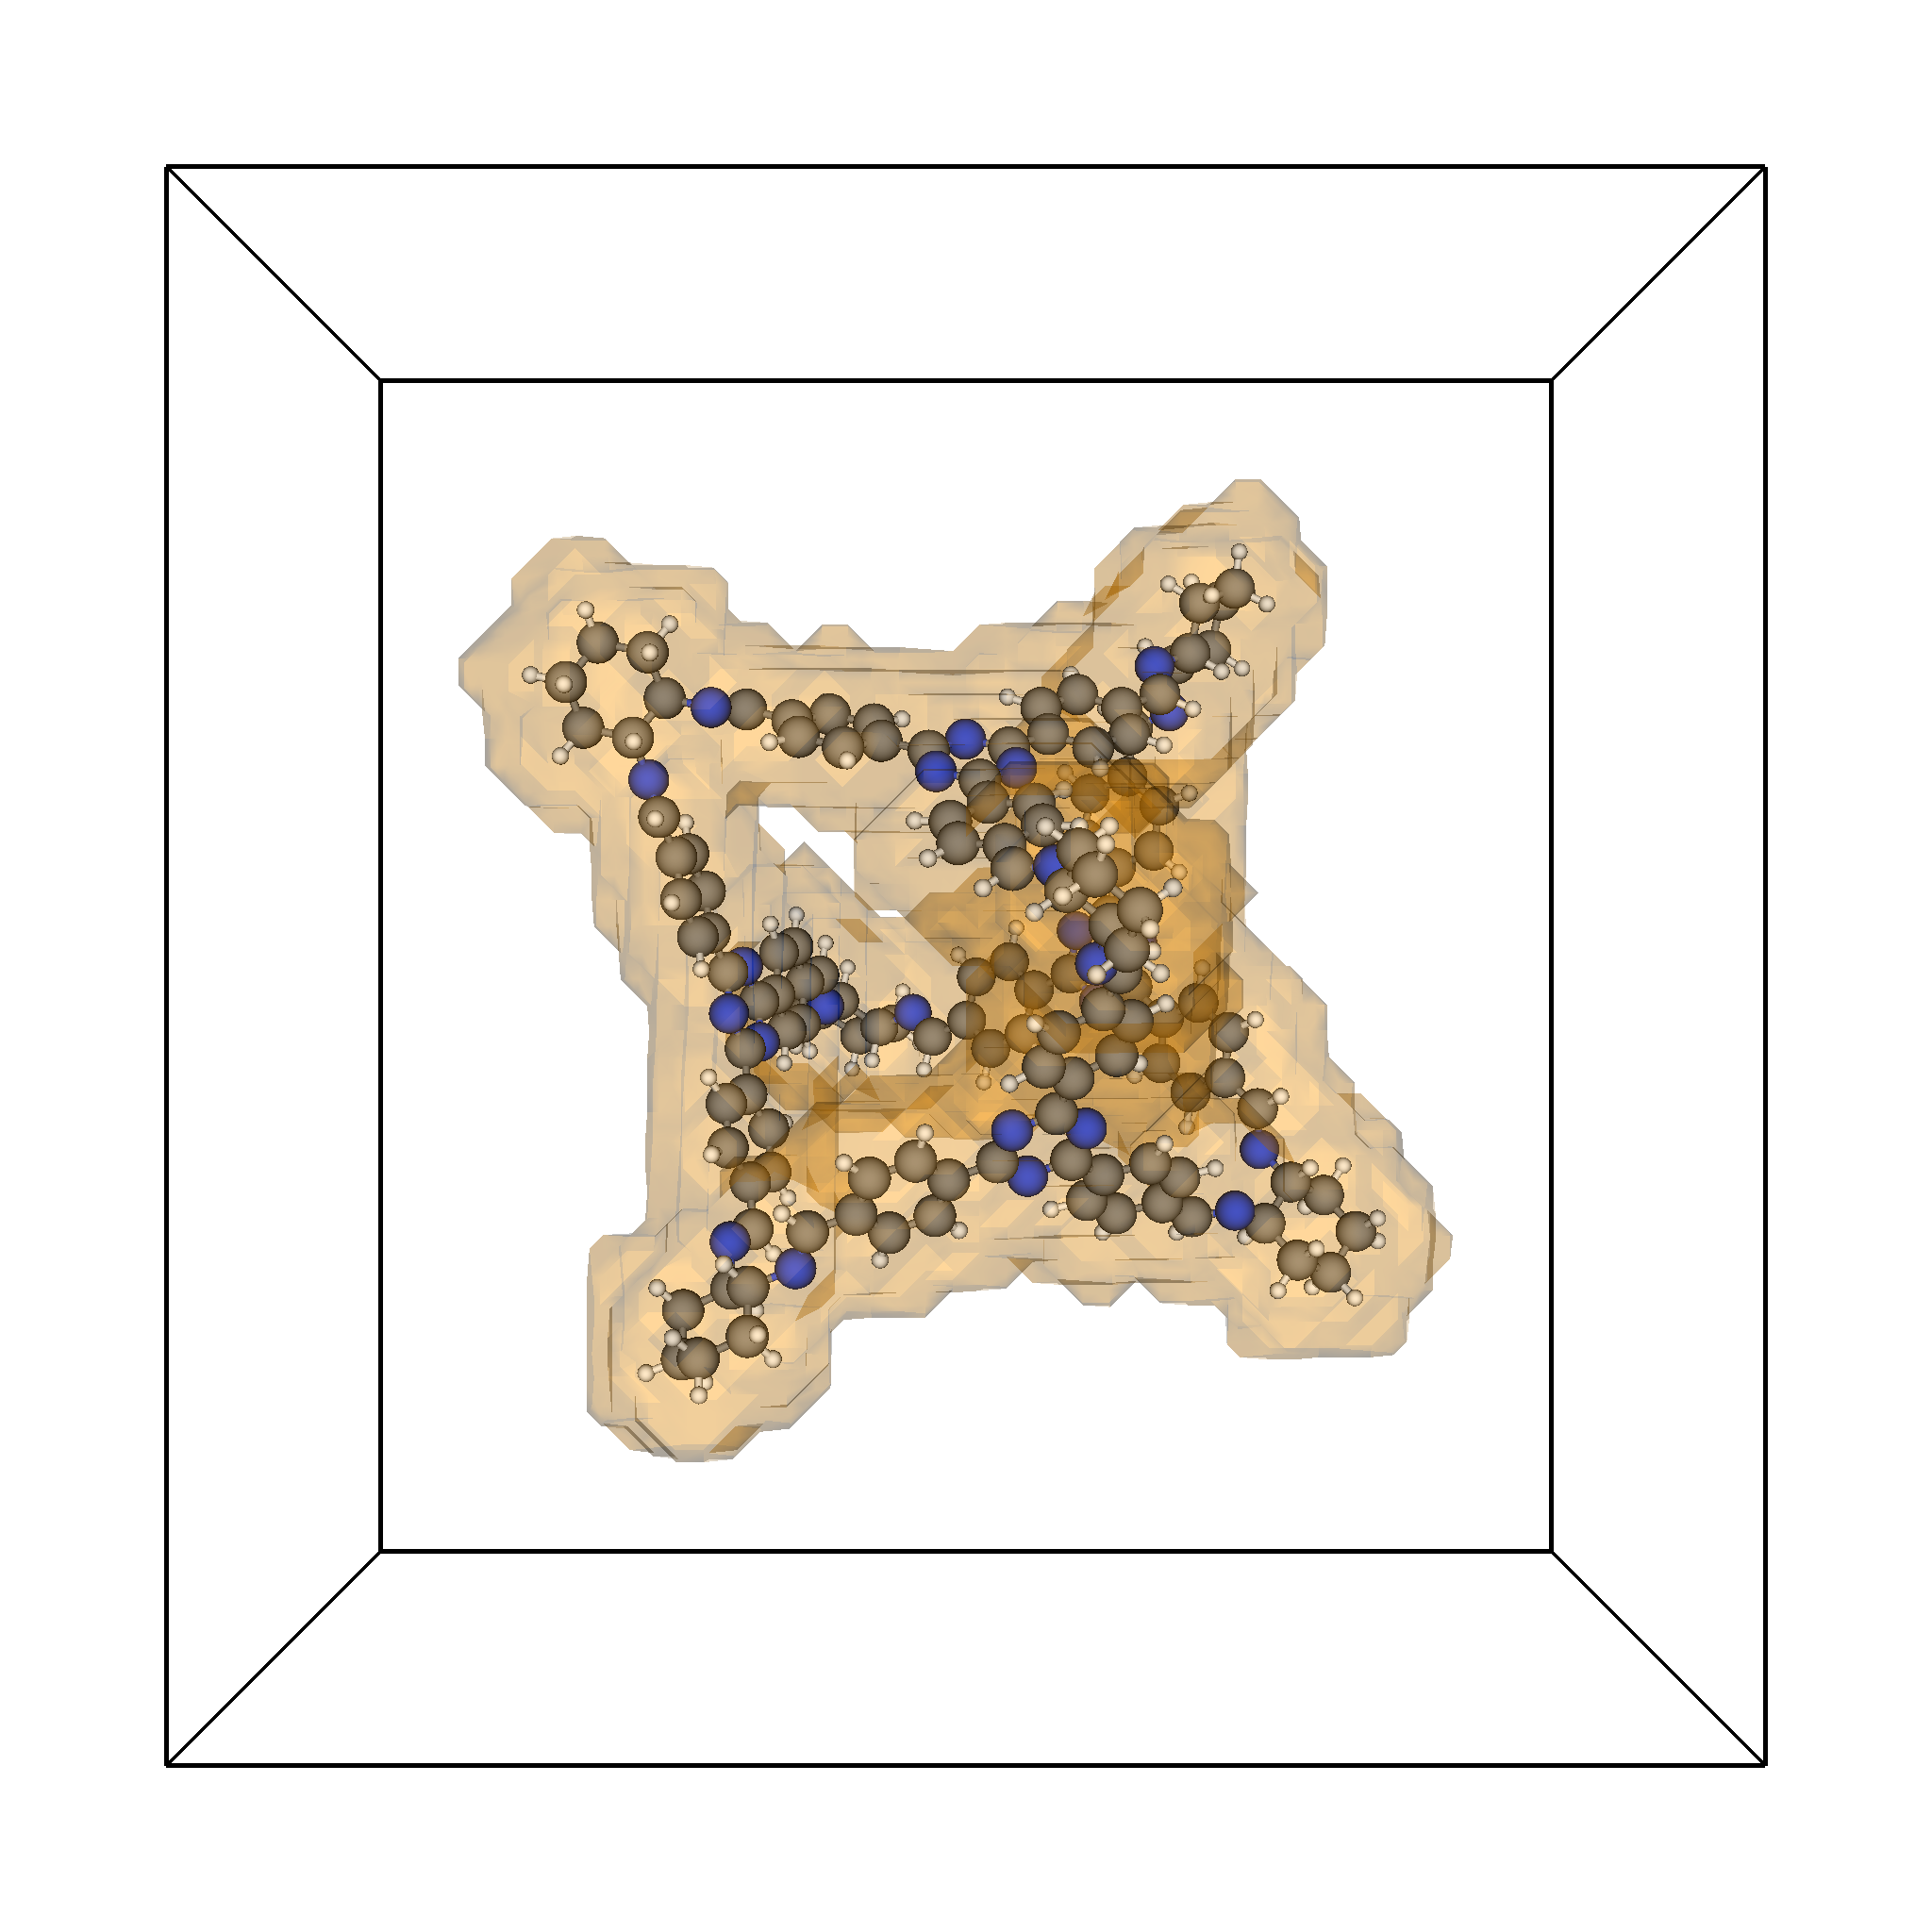
\includegraphics[width=0.3\columnwidth]{WC1_raw.png}}	
	\caption{Example 3D porosity images. {\color{red} (a-f)} The molecular structure of a cage {\color{red} (name and experimental reference in subcaption)} is shown along with a contour (0.5) of the 3D porosity image (orange). Bounding box shows $[-20 \text{ } \angstrom, 20 \text{ } \angstrom]^3$ dimension of the snapshot, consistent for all cages.
	} \label{fig:raw3Dimages}
\end{figure}


\subsection{Classifying a point as void space} We classify a given point in/around a cage as \emph{void space}, as opposed to overlapping an atom of the cage, by computing the potential energy of a helium adsorbate at that point to determine if its interaction with the cage is dominantly repulsive. If and only if the potential energy is less than $k_BT$, with $k_B$ the Boltzmann constant and $T=298$ K the temperature, the point is classified as void space. We model the energetics of the interaction of a helium atom with the atoms of the cage as pairwise additive and with 12-6 Lennard-Jones potentials, taking parameters from the Universal Force Field \cite{rappe1992uff} (geometric mixing rules, cutoff radius 14~$\angstrom$). We use \texttt{PorousMaterials.jl} v0.1.3 \cite{PorousMaterialsJL} to compute the potential energies.

\subsection{Alignment}
\label{sec:alignment}
{\color{red} The singular value decomposition is not equipped to learn rotational and translational invariance of cavity features in the 3D porosity images.} Therefore, we must first consistently align the cages so that each pixel in the 3D porosity image corresponds to the same relative location for each cage. 
Alignment is also required for images of human faces for eigenfaces, so that e.g. the nose and eyes appear in the same region for each face \cite{zhang2008eigenfaces}. First, we translate each cage molecule so that its center of mass is at the origin. {\color{red} Second, we determine how to rotate each cage about its center of mass so that cages with similar cavity shapes are aligned.

As a basis for the rotational alignments, we first generate a set of points that fill and thus characterize the cavity of each cage. We successively insert helium adsorbates at random positions within a sphere circumscribing the cage molecule, rejecting the positions that overlap atoms of the cage and keeping the positions that were classified as void space; this set of points constitutes the \emph{porosity point cloud} of a cage. We bias the insertions towards the center of the cage to emphasize the inner-cavity. See Sec.~\ref{sec:porosity_pt_cld} for more details and Fig.~\ref{fig:porosity_pt_cloud} for example porosity point clouds.

We use the rotational dynamics of the porosity point cloud as a first attempt to align the cages on the basis of their cavity shapes. We rotated each cage so that the principal axes of rotation of its porosity point cloud are aligned with the $x$, $y$, and $z$ Cartesian coordinate axes, with principal moments of inertia arranged in a non-increasing order. See Sec.~\ref{sec:alignment_details}. However, the cavity shapes of most cage molecules exhibit a degree of symmetry so as to render the computed principal axes of rotation sensitive to very small changes in the structure. i.e., the rotational dynamics of most porosity point clouds are approximately those of a sphere or disk, possessing nearly degenerate moments of inertia about the [therefore nearly arbitrary] principal axes of rotation. See Sec.~\ref{sec:degenerate} and Fig.~\ref{fig:irrationallyaligned} for examples of cages irrationally aligned on the basis of the rotational dynamics of their porosity point clouds.
We give the principal axes of rotation authority to align a given cage only if the successive moments of inertia of the porosity point clouds about the principal axes of rotation differ by more than 1\%, the case only for 18/74 cages. For the remaining cages whose porosity point clouds exhibited nearly degenerate principal axes of rotation, we resorted to using a point set registration algorithm, Coherent Point Drift \cite{myronenko2010point}.

We employed Coherent Point Drift\cite{myronenko2010point} to find the optimal rotation matrix to align the porosity point cloud of one cage, $\mathcal{Y}$ to the porosity point cloud of an another cage, $\mathcal{X}$. Briefly, the Coherent Point Drift regards the points in $\mathcal{Y}$ as Gaussian mixture model centroids that generate the points in $\mathcal{X}$. The soft correspondences between points, i.e. the probability that a given point in $\mathcal{X}$ was generated by a Gaussian centered at a given point in $\mathcal{Y}$, are automatically inferred in Coherent Point Drift. The likelihood is maximized by the expectation-maximization (EM) algorithm: the E-step estimates probabilities of correspondence between the points given the current estimate for the rotation matrix and Gaussian variance; the M-step chooses the rotation matrix to minimize the distances between the points in $\mathcal{X}$ and transformed points in $\mathcal{Y}$, weighted by current estimates of the probabilities of correspondence, in addition to making the Gaussians as narrow as possible.

We then iteratively aligned each unaligned cage whose porosity point cloud possesses nearly degenerate principal axes of rotation with an aligned cage. Let $\mathcal{A}$ be the set of 18 cages aligned by the authority of the rotational dynamics of their porosity point clouds and $\mathcal{U}$ be the set of remaining 56 cages not yet aligned. We use Coherent Point Drift to find which cage $u \in \mathcal{U}$ aligns best (the largest likelihood) with a cage in $\mathcal{A}$. We then align this cage $u$ to the cage $a \in \mathcal{A}$ with which it aligns best. We then remove $u$ from the set of unaligned cages $\mathcal{U}$ and add it to the set of aligned cages $\mathcal{A}$ and repeat this process until $\mathcal{U}$ is empty.

In summary, we (i) translated each cage so its center of mass lays at the origin, (ii) generated a point cloud that fills the cavity of each cage, (iii) aligned each cage such that the principal axes of rotation of its porosity point cloud correspond with the Cartesian axes, then (iv) for cages whose porosity point clouds harbor insufficiently distinct principal moments of inertia, align them to another cage, on the basis of their porosity point clouds, using Coherent Point Drift\cite{myronenko2010point}.
}

\subsection{Generating the 3D porosity images}
For each aligned cage molecule, we overlay a regular, $g\times g\times g$ grid of points ($g=50$) that span $40$ $\angstrom$ in each dimension, centered at the center of mass of the cage. The dimension of the $[-20 \text{ } \angstrom, 20 \text{ } \angstrom]^3$ cubic grid of points was chosen as the smallest to encompass all atoms of all the cages. The \emph{3D porosity image} of a cage is then a 3D array; element $(i, j, k)$ is 0 if grid point $(i, j, k)$ is classified as void and 1 otherwise. 

\section{Learning an approximate subspace of porosity images} 

The \emph{raw} representations of porous organic cage molecules as $g\times g \times g$ 3D porosity images lie in a very high-dimensional space ($g^3=125,000$; flattening each image and viewing it as a vector). The main idea in this work is that the intrinsic cavities of porous cage molecules are not randomly distributed in this enormous space, but rather approximately lay in a much lower-dimensional subspace of $\mathbb{R}^{g^3}$. As a revealing thought experiment, consider generating a random 3D porosity image by choosing each pixel as 0 or 1 {\color{red} randomly}; it is extremely likely that this image will not resemble any known cage molecule. That is, the \emph{effective} dimension of 3D porosity images is much lower than $g^3=125,000$. 

We now leverage the singular value decomposition \cite{muller2004singular,kalman1996singularly,strang1993introduction} to learn from the set of 3D porosity images of the cages in Fig.~\ref{fig:cages} an approximate, lower-dimensional subspace in which the 3D porosity images of porous cage molecules lay.
The \emph{eigencages} are a set of orthonormal vectors that span this lower-dimensional subspace; they are ordered in terms of which directions, in the space of all 3D porosity images, account for the most variance among the 3D porosity images of the cages in Fig.~\ref{fig:cages}. Expressing a 3D porosity image as a combination of the eigencages then lends a latent representation of the cage.

\subsection{The data matrix, $\mathbf{A}$} We encapsulate all $c=74$ 3D porosity images of porous cages into a data matrix $\mathbf{A}$. We first flatten the $g\times g\times g$ ($g=25$) images into a set of \emph{raw} vector representations $\{\mathbf{c}_1, \mathbf{c}_2, ..., \mathbf{c}_c\}$, all of which lie in the enormous space $\mathbb{R}^{g^3}$. 
%As we work in Julia \cite{julia}, the 3D array is flattened in column-major order. 
We compute the average 3D porosity image as $\bar{\mathbf{c}}=\frac{1}{c}\sum_{i=1}^c  \mathbf{c}_i$ (visualized later in Fig.~\ref{fig:avg_cage}). Now let $\mathbf{a}_i:=\mathbf{c}_i-\bar{\mathbf{c}}$ be the difference between the porosity image of cage $i$ and the average porosity image. The $c \times g^3$ data matrix $\mathbf{A}$ is then defined by assigning its $i$th row to be $\mathbf{a}_i^T$. As there are many fewer cages than pixels in the 3D porosity images ($c<<g^3$), the data matrix $\mathbf{A}$ is very wide (see Fig.~\ref{fig:data_matrix}).

\subsection{The singular value decomposition (SVD)}
The singular value decomposition (SVD) \cite{muller2004singular,kalman1996singularly,strang1993introduction} enjoys use in genomics \cite{alter2000singular}, recommender systems \cite{koren2008factorization}, and image processing \cite{muller2004singular}. {\color{red} We provide a pedagogical overview of the SVD for the reader's convenience.} We then reason that the SVD of our data matrix $\mathbf{A}$ identifies an approximate lower dimensional subspace in which the 3D porosity images lay and a latent space of the cavities of the porous cages.

\subsubsection{The matrix decomposition}
The singular value decomposition (SVD) of the data matrix $\mathbf{A} \in \mathbb{R} ^{c \times g^3}$ ($g^3 > c$) is:
\begin{equation}
\mathbf{A}=\mathbf{U} \mathbf{\Sigma} \mathbf{V}^T,
\label{eqn:svd}
\end{equation} where $\mathbf{U}$ is a $c \times c$ orthogonal matrix, $\mathbf{\Sigma}$ is an $c\times g^3$ diagonal matrix with the singular values 
$\sigma_1 \geq \sigma_2 \geq \cdots \geq \sigma_{c} \geq 0$ of $\mathbf{A}$ arranged down the diagonal, and $\mathbf{V}$ is a $g^3 \times g^3$ orthogonal matrix. The columns of $\mathbf{U} = [\mathbf{u}_1 \mathbf{u}_2 \cdots \mathbf{u}_c]$ form an orthonormal basis for $\mathbf{R}^c$ and are the \emph{left singular vectors} of $\mathbf{A}$; the columns of $\mathbf{V}=[\mathbf{v}_1 \mathbf{v}_2 \cdots \mathbf{v}_{g^3}]$ form an orthonormal basis for $\mathbb{R}^{g^3}$ and are the \emph{right singular vectors} of $\mathbf{A}$. These left and right singular vectors are eigenvectors of $\mathbf{A}\mathbf{A}^T$ and $\mathbf{A}^T\mathbf{A}$, respectively; the non-zero singular values are the square roots of the [shared] non-zero eigenvalues of $\mathbf{A}\mathbf{A}^T$ and $\mathbf{A}^T\mathbf{A}$. Given that the latter matrix is proportional to the sample covariance matrix, we are essentially conducting principal component analysis \cite{strang1993introduction}, identifying the most significant directions of variance among the 3D porosity images.

\begin{figure}
\centering
	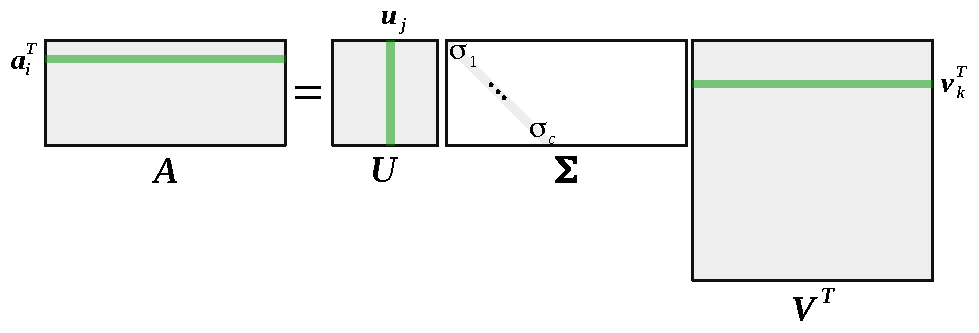
\includegraphics[width=0.75\columnwidth]{svd-crop.pdf}
	\caption{The full singular value decomposition of $\mathbf{A}$ in eqn.~\ref{eqn:svd}. {\color{red} Relevant rows/columns are colored and labeled.}
	} \label{fig:svd}
\end{figure}

Given that the matrix $\mathbf{A}$ is rank $r$ and $\mathbf{\Sigma}$ in eqn.~\ref{eqn:svd} has many columns of zeros because our matrix is wide (see Fig.~\ref{fig:svd}), we can write eqn.~\ref{eqn:svd} in a reduced form:
\begin{equation}
\mathbf{A}=\mathbf{U}_r \mathbf{\Sigma}_r \mathbf{V}_r^T,
\label{eqn:svd_r}
\end{equation} where now $\mathbf{\Sigma}_r$ is a diagonal $r\times r$ matrix that contains only the $r$ non-zero singular values of $\mathbf{A}$ down its diagonal in a non-increasing order, $\mathbf{U}_r=[\mathbf{u}_1\hspace{1mm} \mathbf{u}_2\hspace{1mm} \cdots \hspace{1mm}\mathbf{u}_r]$ is a $c\times r$ matrix, and $\mathbf{V}_r=[\mathbf{v}_1\hspace{1mm} \mathbf{v}_2\hspace{1mm}\cdots \hspace{1mm}\mathbf{v}_r]$ is a $g^3\times r$ matrix. Writing eqn.~\ref{eqn:svd_r} using an outer product expansion expresses $\mathbf{A}$ as a sum of rank-one matrices:
\begin{equation}
\mathbf{A} = \displaystyle \sum_{i=1}^r \sigma_i \mathbf{u}_i\mathbf{v}_i^T.
\label{eqn:sum_rank_1}
\end{equation} The singular values appear in eqn.~\ref{eqn:sum_rank_1} as weights on the rank-one matrices, formed by the outer product of two unit vectors, used to construct the matrix $\mathbf{A}$. This emphasizes that the singular vectors are ordered in terms of significance.

We numerically compute the singular value decomposition using the \texttt{svd} function in Julia \cite{julia}.

\subsubsection{A geometric view of SVD}
A useful geometric view of the SVD follows by considering how $\mathbf{A}$ maps a unit hypersphere in $\mathbb{R}^{g^3}$ into $\mathbb{R}^c$. We can express any point $\mathbf{x}_s\in \mathbb{R}^{g^3}$ on the unit hypersphere as a linear combination of the right singular vectors:
\begin{equation}
\mathbf{x}_s = \alpha_1 \mathbf{v}_1 + \alpha_2 \mathbf{v}_2 + \cdots + \alpha_{g^3} \mathbf{v}_{g^3},
\end{equation} such that $\sum_{i=1}^{g^3} \alpha_i^2 = 1$ to enforce $||\mathbf{x_s}||=1$. Upon multiplication by $\mathbf{A}$, the point $\mathbf{x}_s$ is transformed to a new vector:
\begin{equation}
\mathbf{A} \mathbf{x}_s = \alpha_1 \sigma_1 \mathbf{u}_1 + \alpha_2 \sigma_2 \mathbf{u}_2 + \cdots + \alpha_r \sigma_r \mathbf{u}_r.
\label{eqn:ellipse}
\end{equation} This follows from $\mathbf{A} \mathbf{v}_i = \sigma_i \mathbf{u}_i$ for $i=1,2,...,r$ and $\mathbf{A} \mathbf{v}_i = \mathbf{0}$ for $i=r+1,...,g^3$. Eqn.~\ref{eqn:ellipse} describes an $r$-dimensional ellipsoid lying in $\mathbb{R}^c$, whose principal semi-axes are in the direction of $\mathbf{u}_i$ with lengths of $\sigma_i$ for $i=1,...,r$. Therefore, multiplication by $\mathbf{A}$ deforms the unit hypersphere in $\mathbb{R}^{g^3}$ by first collapsing $g^3-r$ dimensions, then stretching/compressing it along the remaining $r$ dimensions, then rotating it, resulting in an $r$-dimensional ellipsoid that lays in $\mathbb{R}^c$. The SVD recovers the directions of the principal semi-axes of this ellipsoid, $\{\mathbf{u}_i\}$, and their lengths, $\{\sigma_i\}$, as well as each vector $\mathbf{v}_i$ that is mapped to $\sigma_i \mathbf{u}_i$. The vectors $\{\mathbf{u}_i\}$ are orthonormal and, remarkably, so are the set of vectors $\{\mathbf{v}_i\}$.


%From the geometric view, the largest singular value indicates the maximum a unit vector can be dilated by multiplying by $\mathbf{A}$ because it is the length of the longest principal semi-axis of the ellipsoid:
%\begin{equation}
%\sigma_1 = \sup_{||\mathbf{x}||=1} ||\mathbf{A}\mathbf{x}||. 
%\end{equation} The expression on the right is defined as the operator norm of $\mathbf{A}$. Similarly, the maximum amount that a vector is contracted after multiplying by $\mathbf{A}$ is the least singular value, the length of the smallest principal semi-axis of the ellipsoid:
%\begin{equation}
%\sigma_r = \inf_{||\mathbf{x}||=1} ||\mathbf{A}\mathbf{x}||. 
%\end{equation}

\subsubsection{Low-rank-$\nu$ approximation $\mathbf{A}_\nu$ to the data matrix $\mathbf{A}$}
Now, we employ the SVD to compress the data matrix $\mathbf{A}$ by finding a low-rank approximation. We define the ``best'' rank $\nu<r$ approximation to $\mathbf{A}$, $\mathbf{A}_\nu$, as the one where $||\mathbf{A}-\mathbf{A}_\nu||_F$ is minimized, where $||\cdot||_F$ is the Frobenius norm. One can show that the optimal rank-$\nu$ approximator is:
\begin{equation}
\mathbf{A}_\nu =  \displaystyle \sum_{i=1}^\nu \sigma_i \mathbf{u}_i\mathbf{v}_i^T.
\label{eq:Anu}
\end{equation} Comparing to eqn.~\ref{eqn:sum_rank_1}, the optimal rank $\nu$ approximator is obtained by setting the singular values $\sigma_{\nu+1}=\sigma_{\nu +2} = \cdots = \sigma_r = 0$. Aided by our geometric interpretation, we are approximating the linear transformation governed by $\mathbf{A}$ by collapsing the shortest principal axes of the ellipsoid in eqn.~\ref{eqn:ellipse}; justified intuitively, an ellipse e.g. in 2D is best-approximated by its longest principal axis. The relative error in the approximation is:
\begin{equation}
\frac{||\mathbf{A}-\mathbf{A}_\nu||_F}{||\mathbf{A}||_F} = \sqrt{\frac{ \displaystyle \sum_{i=\nu+1}^r \sigma_i^2}{\displaystyle \sum_{i=1}^r \sigma_i^2
}}.
\label{eq:relative_error}
\end{equation} From a geometric standpoint, the relative error is related to the lengths of the principal semi-axes that we collapse in approximating the $r$-dimensional ellipsoid in eqn.~\ref{eqn:ellipse} with a $\nu$-dimensional ellipsoid and how they compare to the longest principal semi-axes retained.

\subsubsection{Interpreting the SVD for void space images of porous cage molecules}
The data matrix $\mathbf{A}$ encapsulates the 3D porosity images of all 74 porous cage molecules. 
% The columns of $\mathbf{A}$ can be interpreted as representations of each pixel in terms of a combination of the $c$ cages. 
We showed that we can approximate the data matrix $\mathbf{A}$ with a lower-rank approximant $\mathbf{A}_\nu$ in eqn.~\ref{eq:Anu}. 
%Geometrically, this corresponds to approximating an $r$-dimensional ellipsoid by collapsing its smallest principal semi-axes. 
The right singular vectors $\{\mathbf{v}_i\}$ lie in the space of all 3D porosity images. As only the first $\nu$ right singular vectors appear in the approximant in eqn.~\ref{eq:Anu}, the best $\nu$-dimensional subspace of 3D porosity images is thus spanned by the orthonormal set of vectors $\mathbf{v}_1, \mathbf{v}_2, ..., \mathbf{v}_\nu$. Analogous to eigenfaces \cite{turk1991face,muller2004singular}, we declare this set of vectors, which are fictitious 3D porosity images [well, with $\bar{\mathbf{c}}$ subtracted and normalized to have magnitude unity] discovered by SVD, the \emph{eigencages}. Algebraically, eqn~\ref{eq:Anu} approximates the flattened 3D porosity image of cage $k$ as:
\begin{equation}
\mathbf{c}_k^T\approx \bar{\mathbf{c}}^T + \sum_{i=1}^\nu \sigma_i \mathbf{u}_i[k] \mathbf{v}_i^T,
\label{eq:latent_space_view}
\end{equation} confirming cage $k$ is approximately a linear combination of the eigencages $\mathbf{v}_1, \mathbf{v}_2, ..., \mathbf{v}_\nu$ with weights composed of the $k$th row of $\mathbf{U}_\nu$ and the singular values $\sigma_1, \sigma_2 ,...,\sigma_\nu$. In this linear combination, the singular value $\sigma_i$ appears as a weight to its corresponding eigencage $\mathbf{v}_i$, indicating a hierarchy of importance of the eigencages and justifying discarding the singular vectors with smaller singular values in the approximant in eqn.~\ref{eq:Anu}. Instead of a $g^3$-dimensional 3D porosity image, each porous organic cage molecule can be represented by its composition of $\mathbf{v}_1, \mathbf{v}_2, ..., \mathbf{v}_\nu$ given in eqn.~\ref{eq:latent_space_view}. The \emph{latent representation} of the 3D porosity image of cage $k$ is therefore row $k$ of $\mathbf{U}_\nu \mathbf{\Sigma}_\nu$. See Fig.~\ref{fig:svd_approx}.

\begin{figure}
\centering
	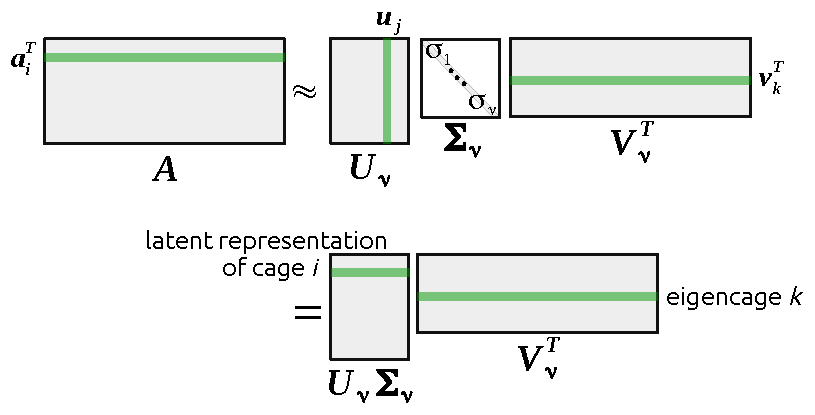
\includegraphics[width=0.75\columnwidth]{svd_approx-crop.pdf}
	\caption{The low rank approximant $\mathbf{A}_\nu \approx \mathbf{A}$ in eqn.~\ref{eq:Anu}. Compare to Fig.~\ref{fig:svd}. Eigencage $k$ is row $k$ of $\mathbf{V}_\nu^T$. The latent representation of cage $i$ is row $i$ of $\mathbf{U}_\nu \mathbf{\Sigma}_\nu$.
	} \label{fig:svd_approx}
\end{figure}

We choose the dimension of the latent space $\nu$ as the smallest such that the relative error in eqn.~\ref{eq:relative_error} is less than 15\%, leading to $\nu=22$. See Fig.~\ref{fig:relative_err_with_svs}. As we have $c=74$ cages, $\nu=c=74$ would exactly reconstruct all cages in our cage data set. Thus, this compression to $\nu=22$ dimensions is a 70\% compression of the 3D porosity images of the cages while incurring only a 15\% error in reconstructing the cages. The distribution of the singular values of $\mathbf{A}$ is shown in Fig.~\ref{fig:distn_of_svs}.

To summarize, the singular value decomposition, in an unsupervised manner, learns:
\begin{itemize}
\item the best approximate $\nu$-dimensional subspace of $\mathbb{R}^{g^3}$ in which the 3D images of the porosity of cage molecules lay. This subspace is spanned by the set of orthonormal right singular vectors $\mathbf{v}_1, \mathbf{v}_2, ..., \mathbf{v}_\nu$, ranked in terms of importance, which we declare as \emph{eigencages}.
\item a $\nu$-dimensional \emph{latent space} of porous organic cage molecules defined by the weights used to approximately construct a 3D porosity image from a linear combination of the eigencages. The $\nu$-dimensional \emph{latent representation} of cage $i$ is the $i$th row of $\mathbf{U}_\nu \mathbf{\Sigma}_\nu$.
\end{itemize}


\subsection{The eigencages} The eigencages-- the rows of $\mathbf{V}_\nu^T$ (see Fig.~\ref{fig:svd_approx})-- are an orthonormal basis for the approximate lower dimensional subspace in which all 3D porosity images lay and are ordered in terms of importance. The eigencages are the directions in 3D porosity image space that account for the most variance among the 3D porosity images in the dataset \cite{strang1993introduction}. We visualize the first (and most important) six eigencages in Fig.~\ref{fig:eigencages}. As eqn.~\ref{eq:latent_space_view} illustrates, the eigencages express deviations from the average 3D porosity image $\bar{\mathbf{c}}$, whose contours are shown in Fig.~\ref{fig:avg_cage}. Thus, the eigencages possess contours at both positive and negative values. The periphery of the first eigencage $\mathbf{v}_1$ in Fig.~\ref{fig:eigencage1} exhibits radial symmetry; as Fig.~\ref{fig:first_component_captures_pore_diameter} indicates, $\mathbf{v}_1$ is used heavily to describe how the cavity diameter of a given cage differs from the average cage in Fig.~\ref{fig:avg_cage}. The second and third eigencages appear to capture windows to the cavities and moieties that protrude from the core of the cage molecule. The fifth and sixth eigencages possess lobes likely describing windows but are difficult to reconcile with our intuition of how to describe the shape of a cage molecule, highlighting that a human-engineered feature of porous organic cages is unlikely to be optimal in compressing the information about a cage cavity into a low-dimensional representation.

\begin{figure}
% made with image zoom 1.4. see saved VisIT session in data/grids. mesh width 4, see snapshot.vtk
	\centering
	\subfloat[][$\bar{\mathbf{c}}$]{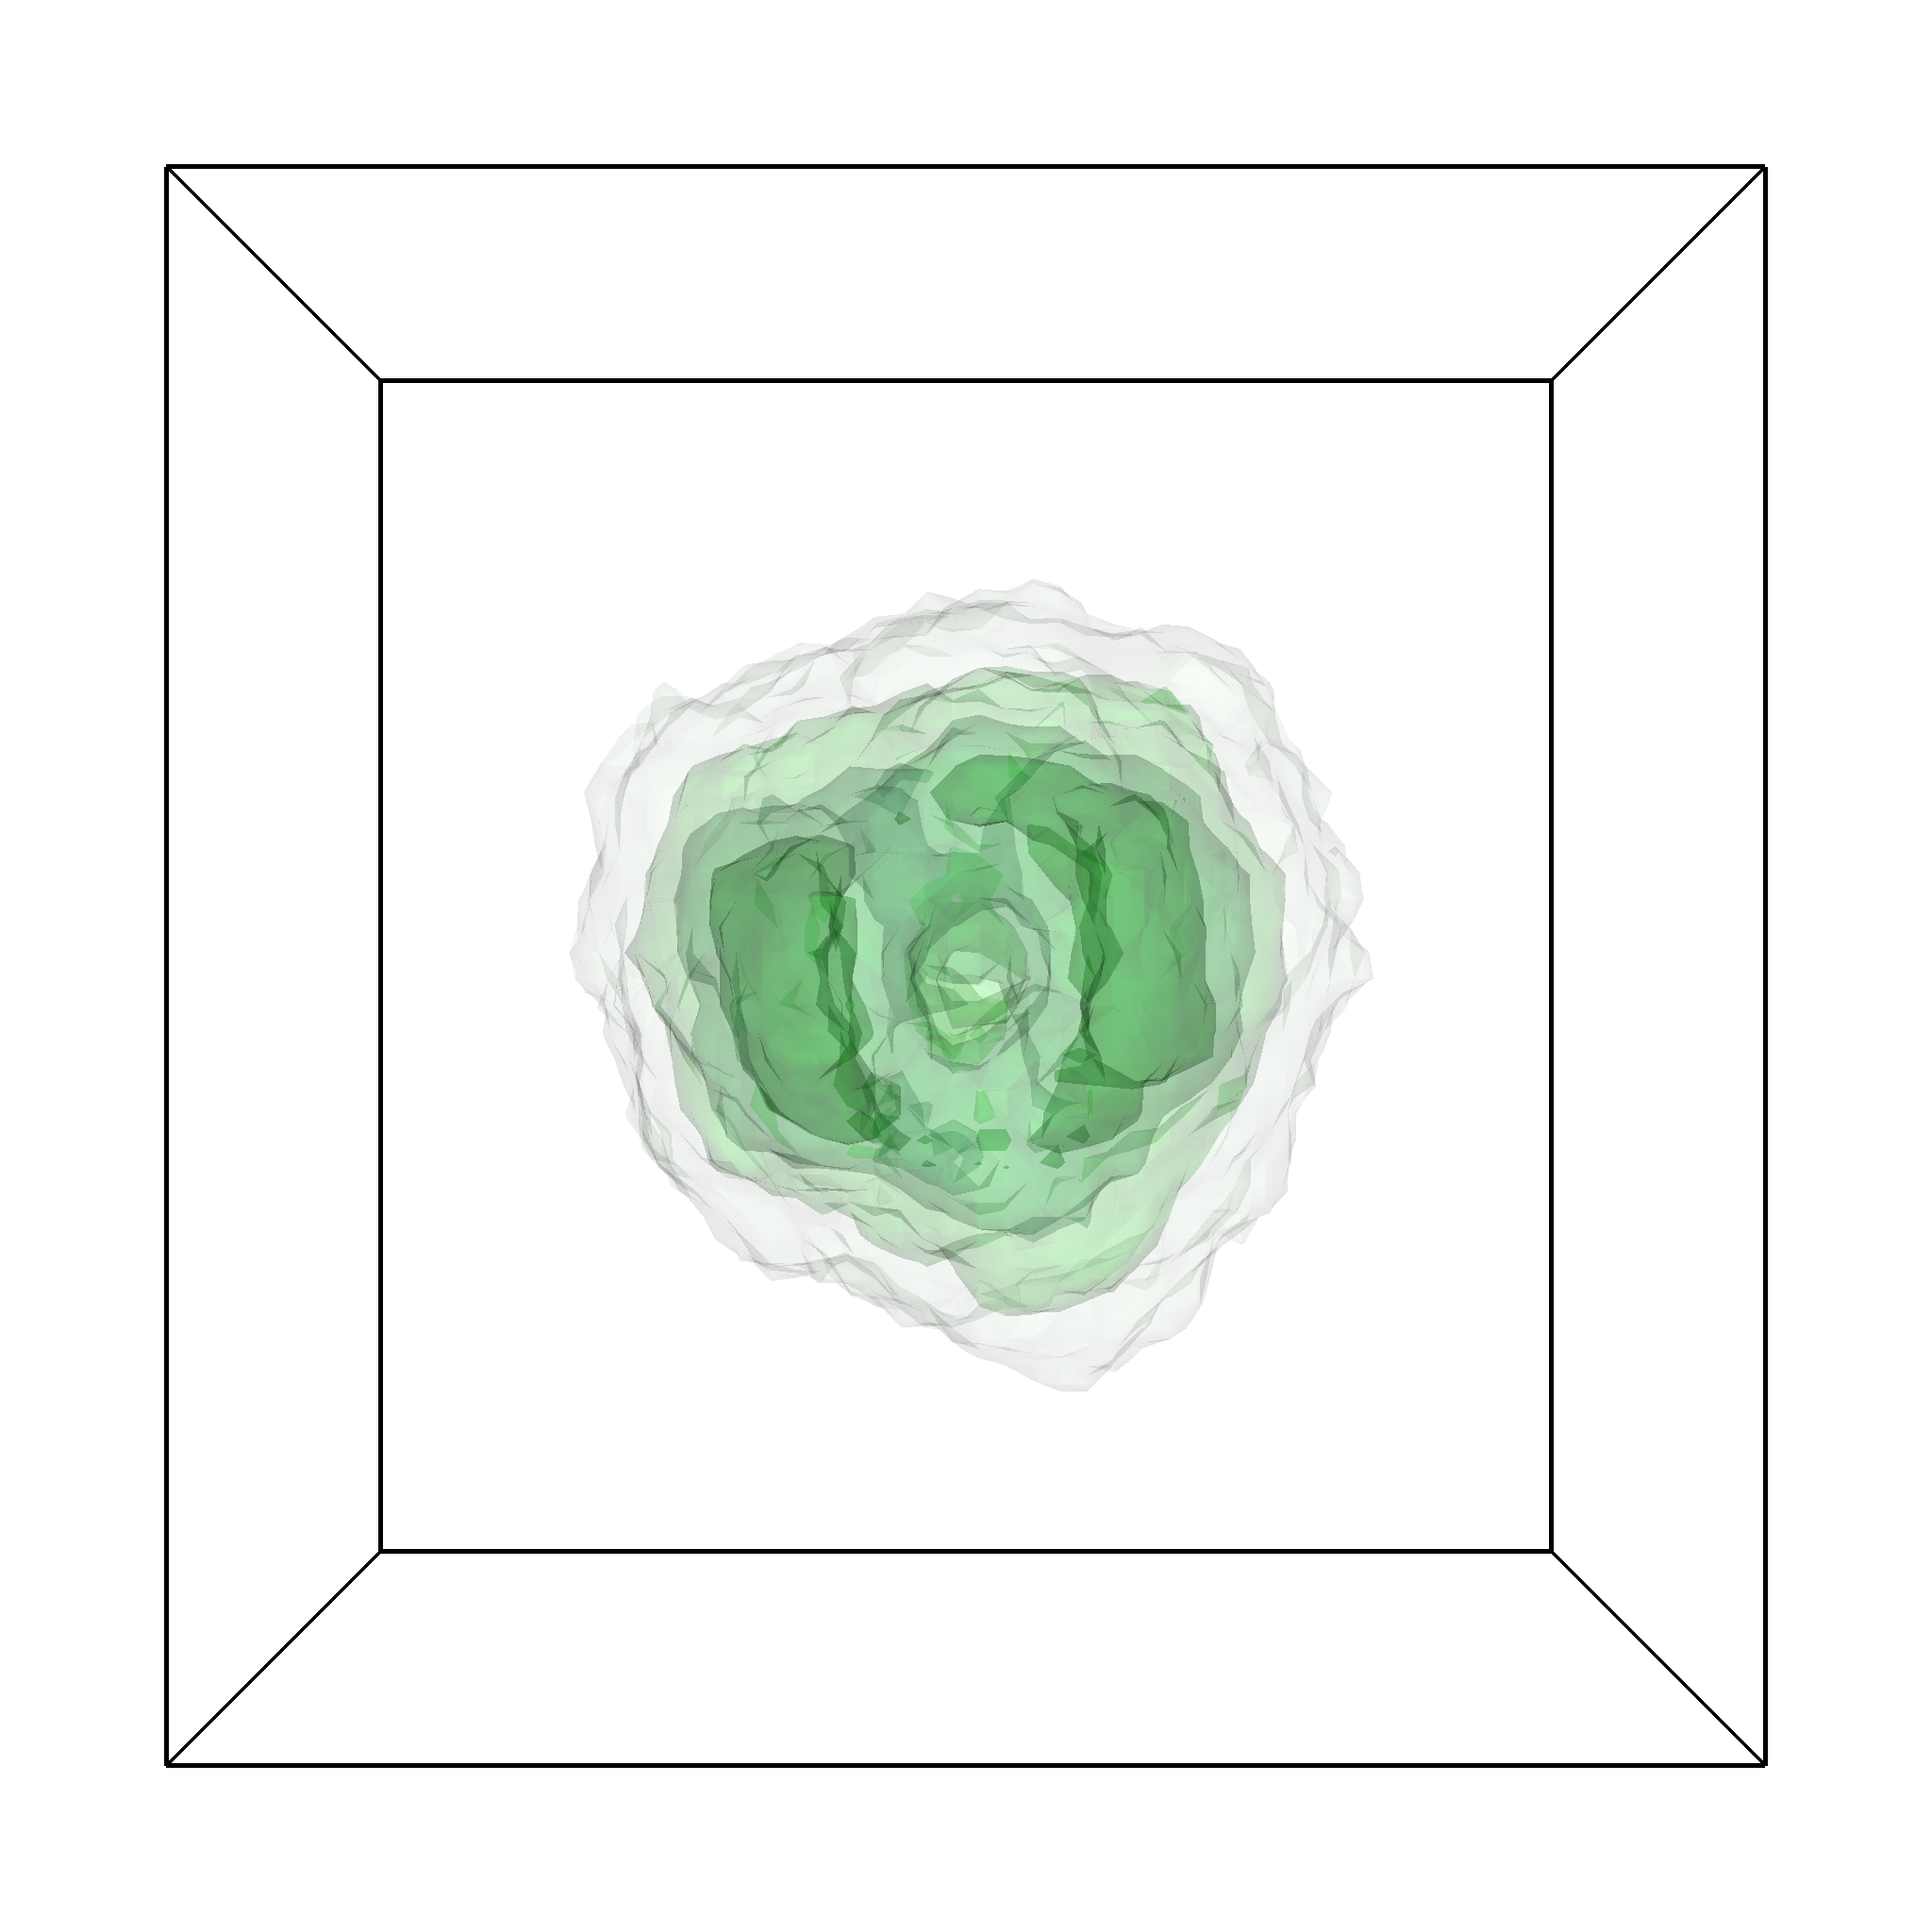
\includegraphics[width=0.3\columnwidth]{average_cage.png}\label{fig:avg_cage}}
	\\
	\subfloat[][$\mathbf{v}_1$]{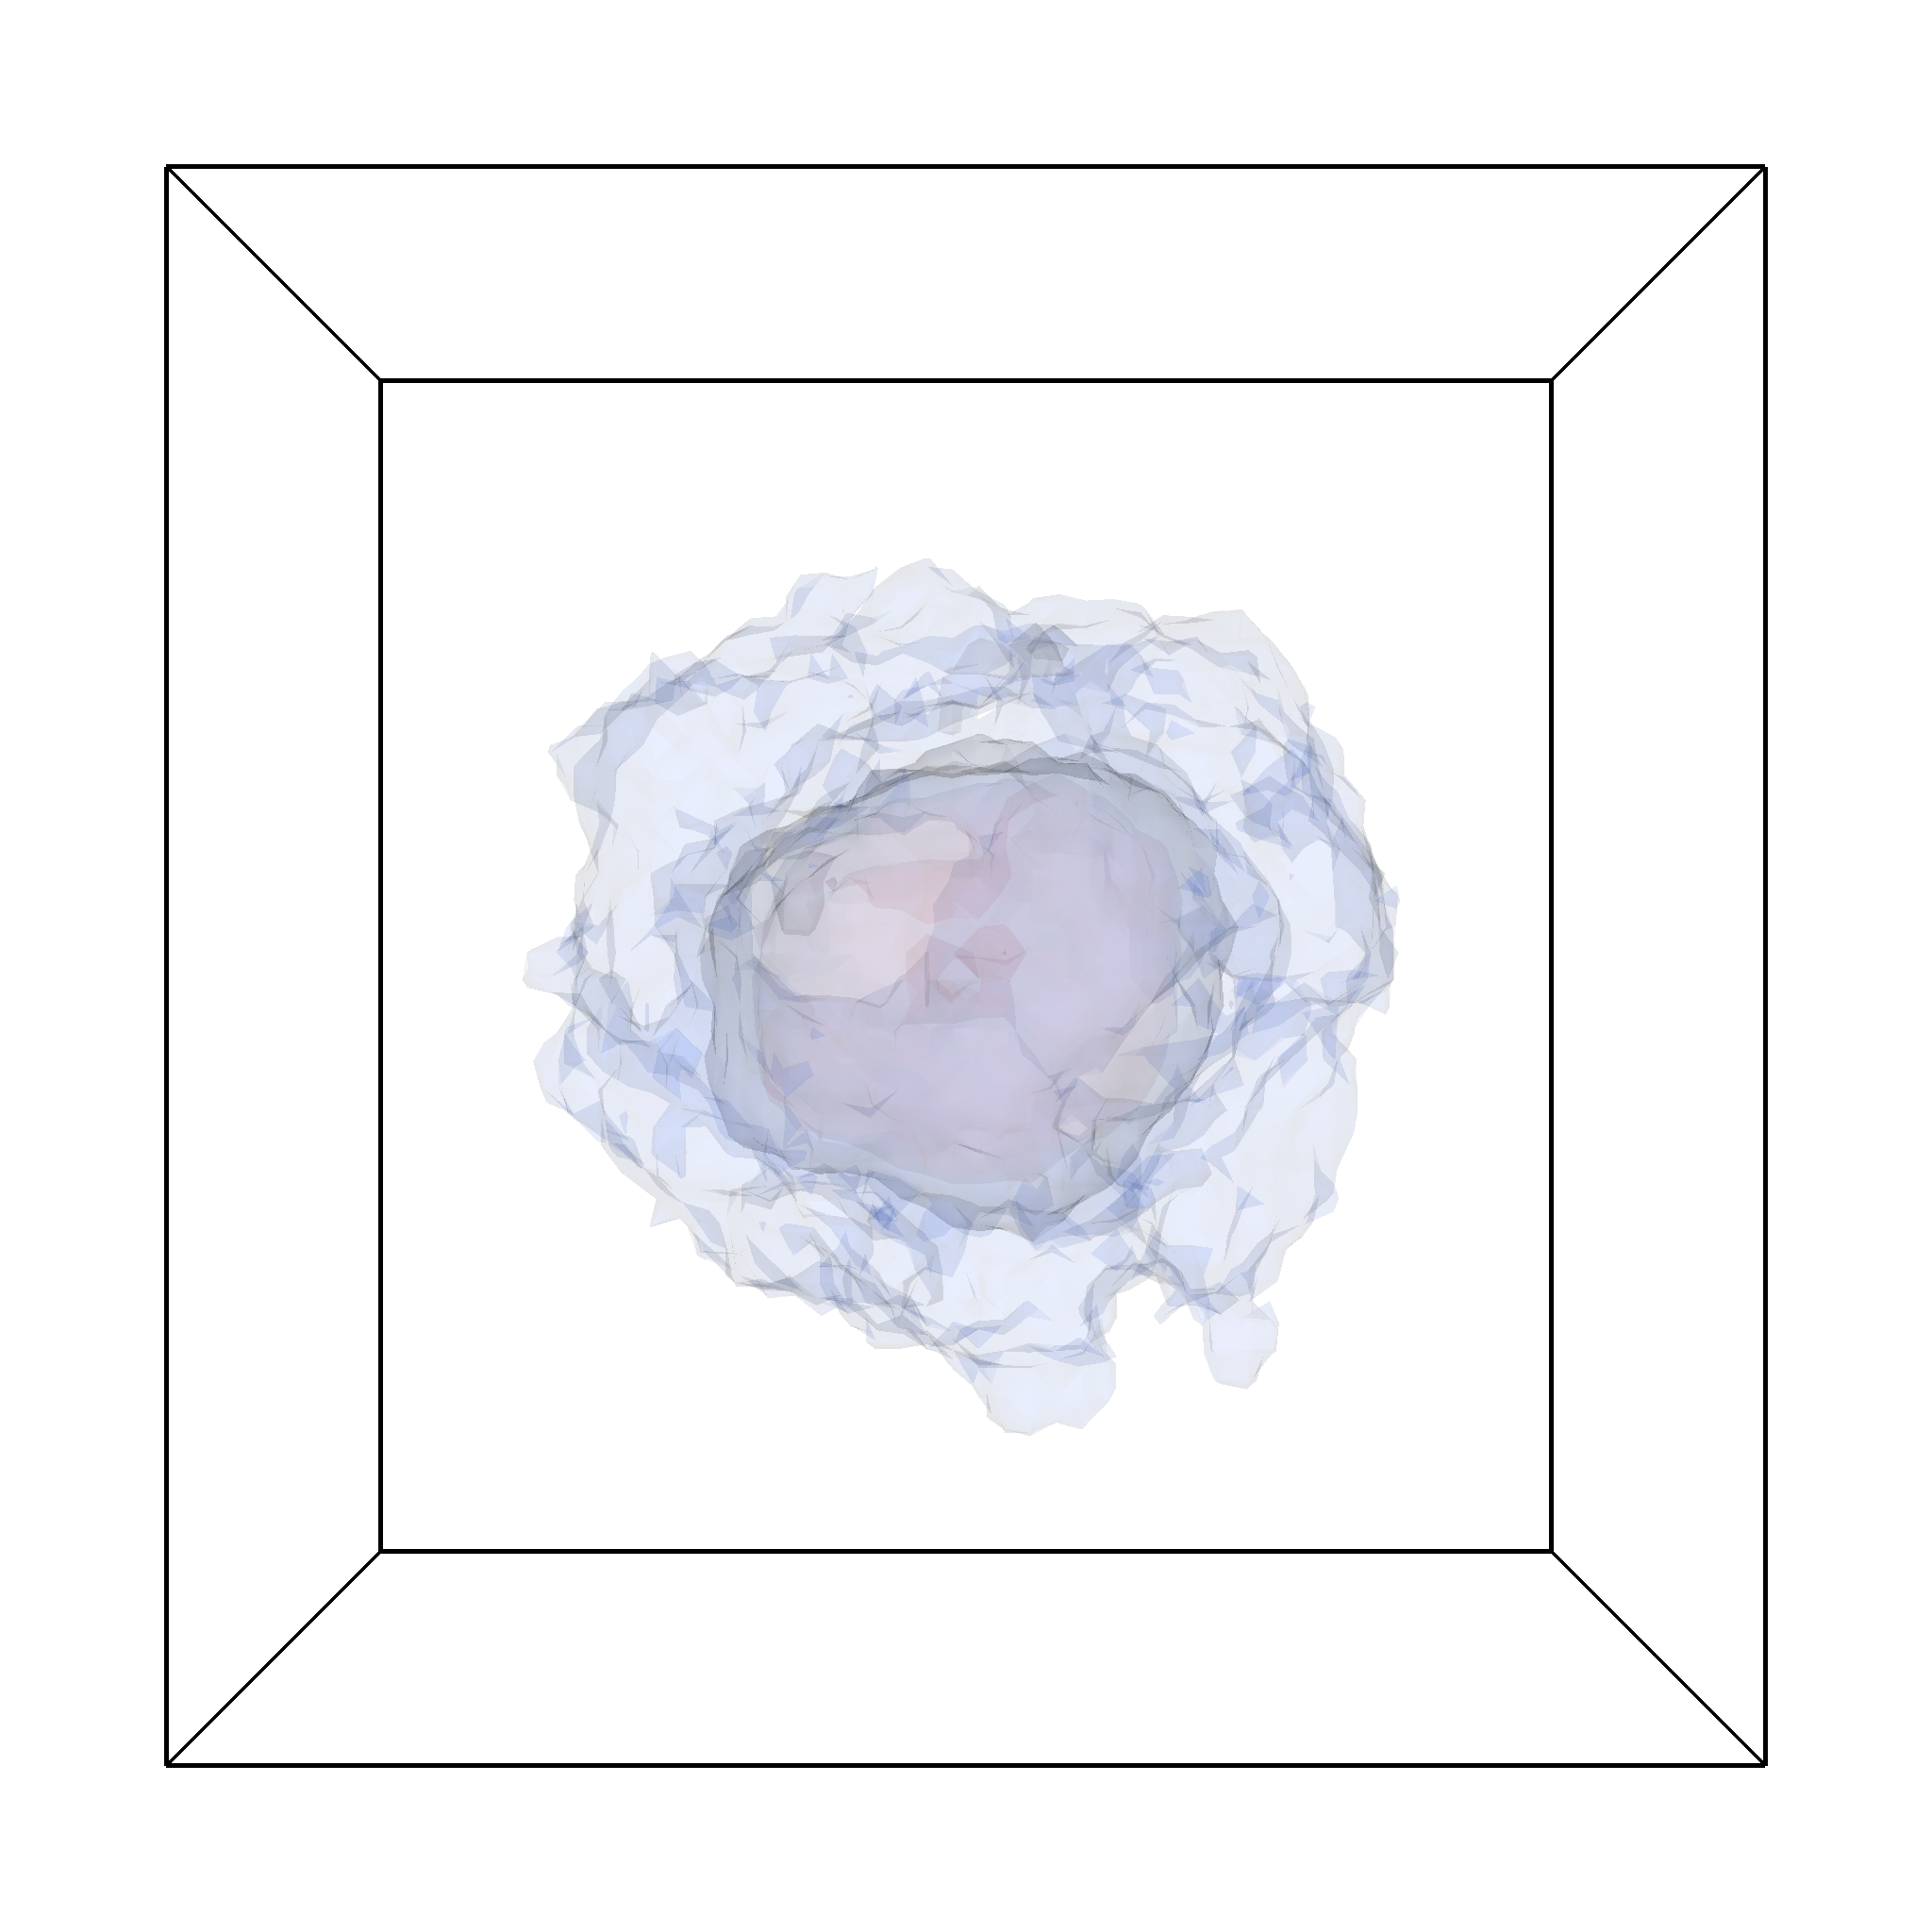
\includegraphics[width=0.272\columnwidth]{eigencage1.png}\label{fig:eigencage1}}
	\subfloat[][$\mathbf{v}_2$]{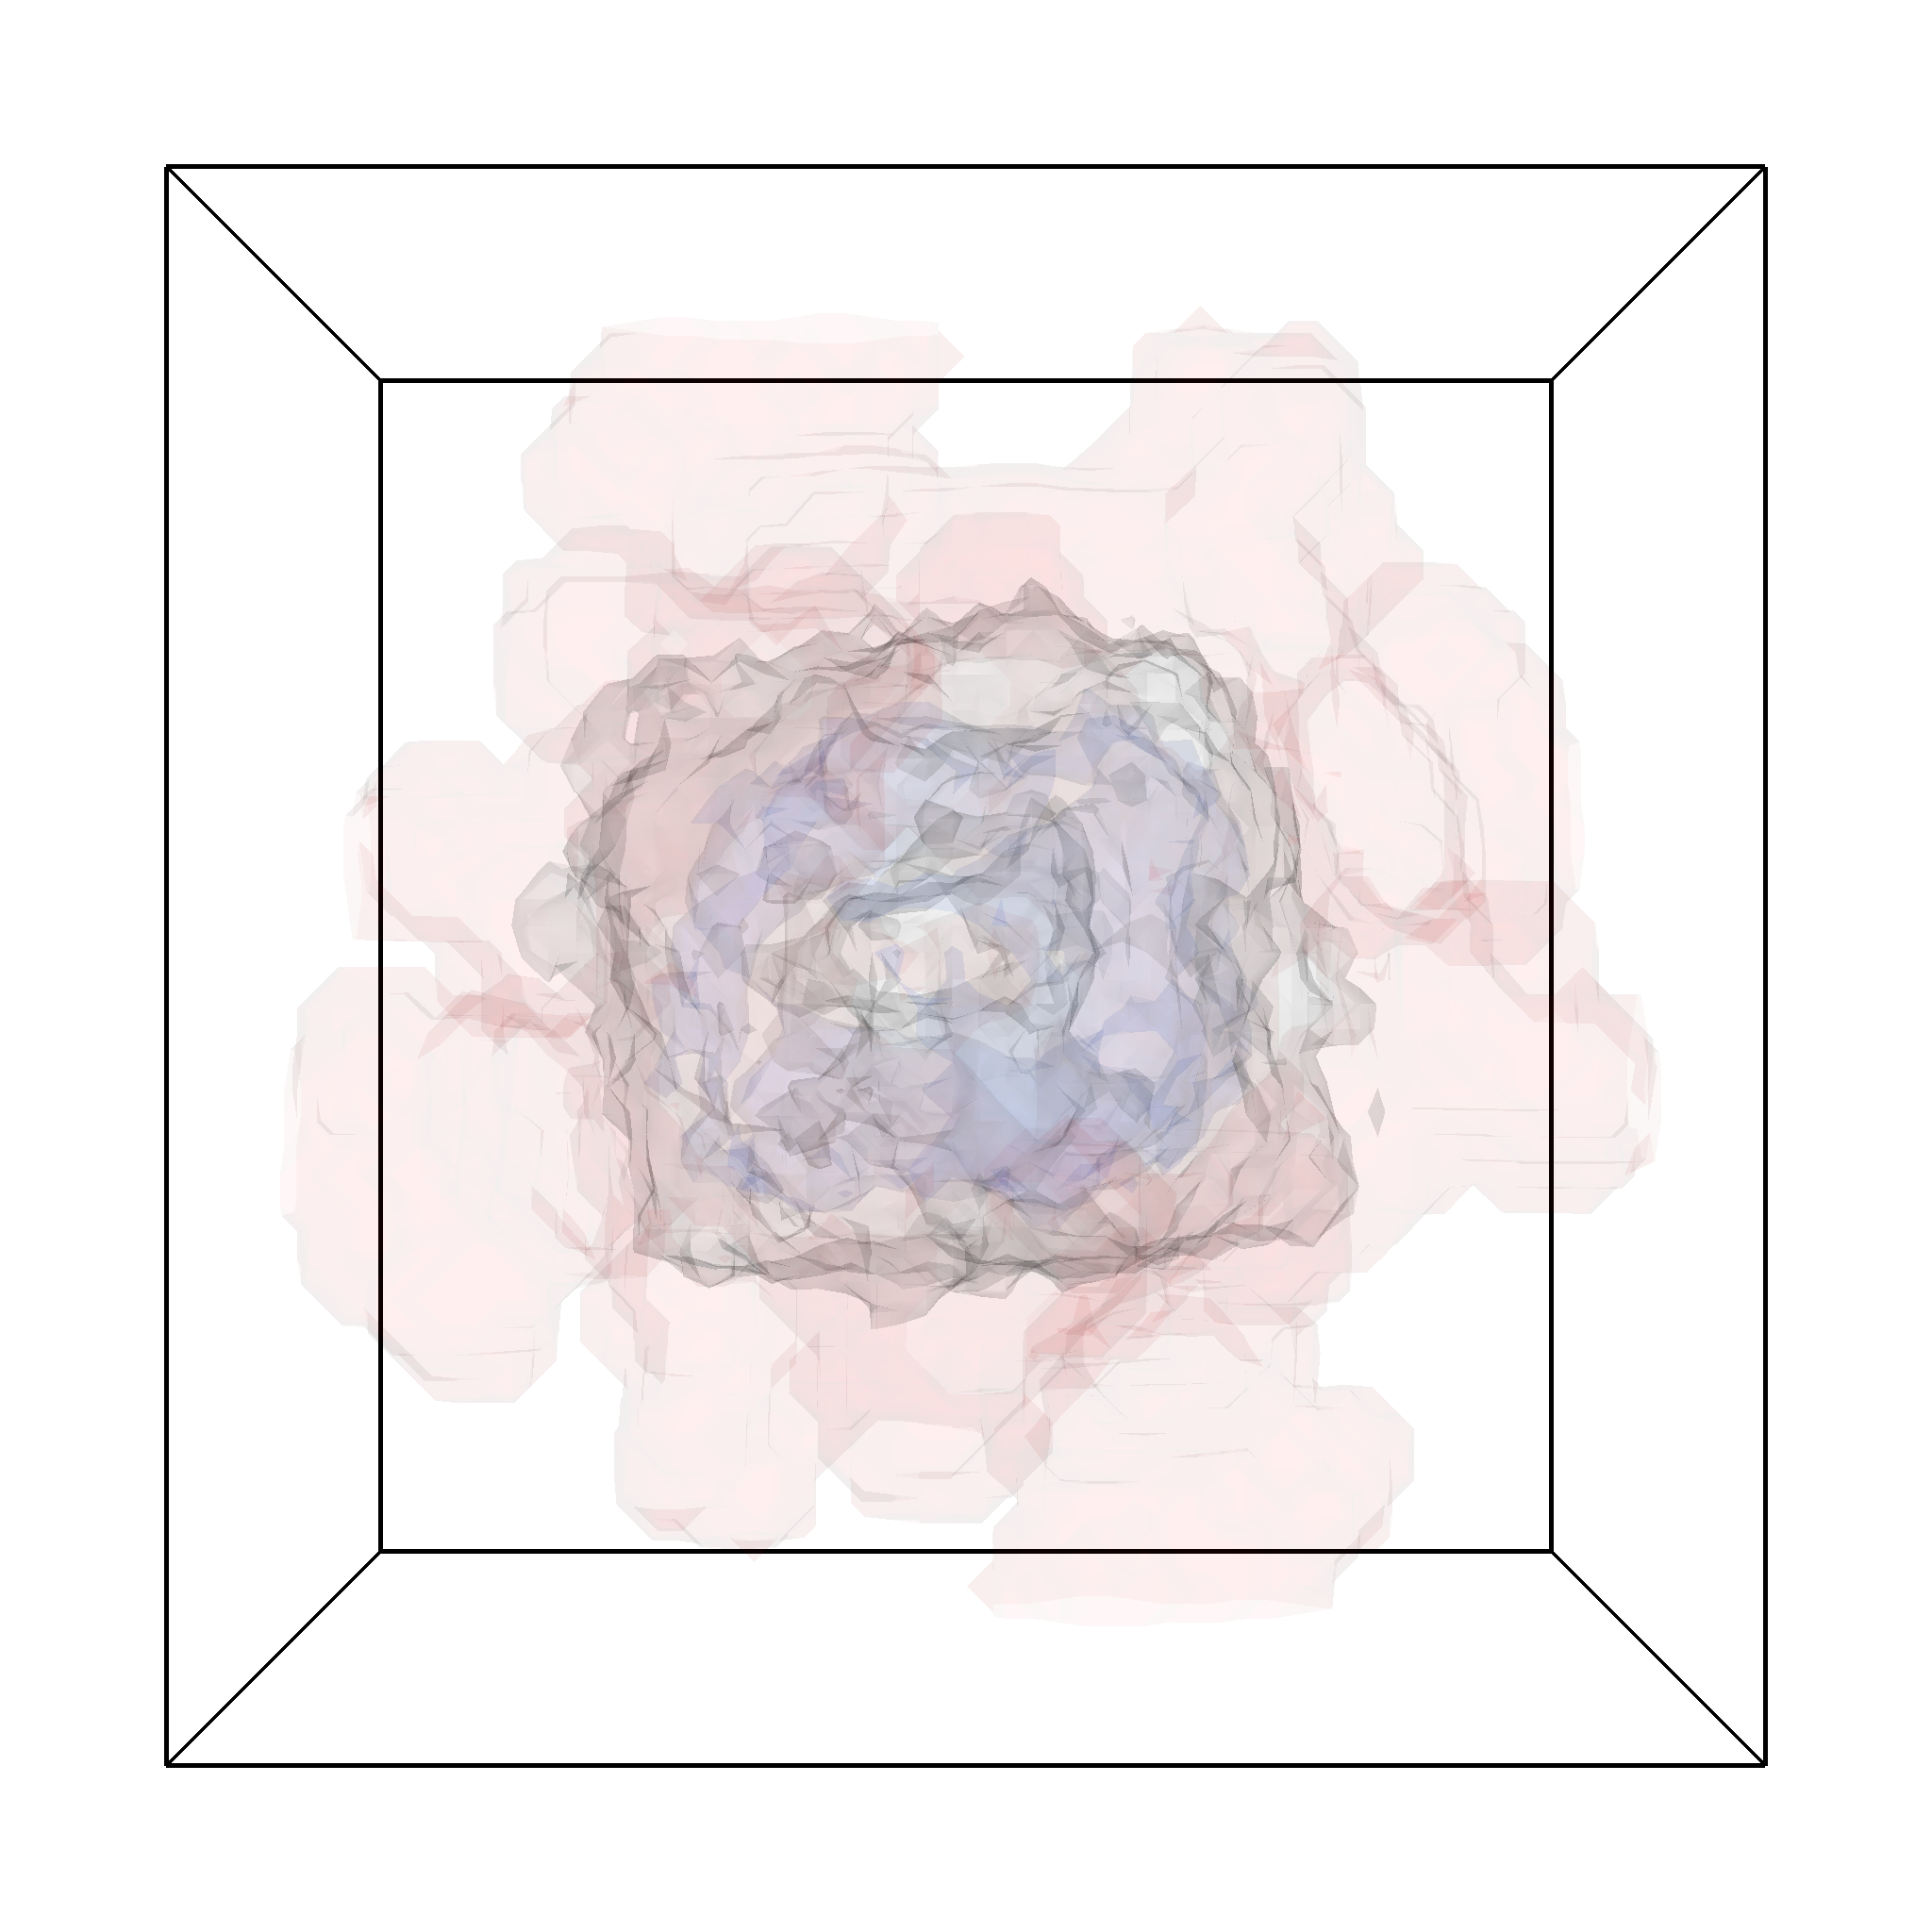
\includegraphics[width=0.272\columnwidth]{eigencage2.png}}
		\qquad
	\subfloat[][$\mathbf{v}_3$]{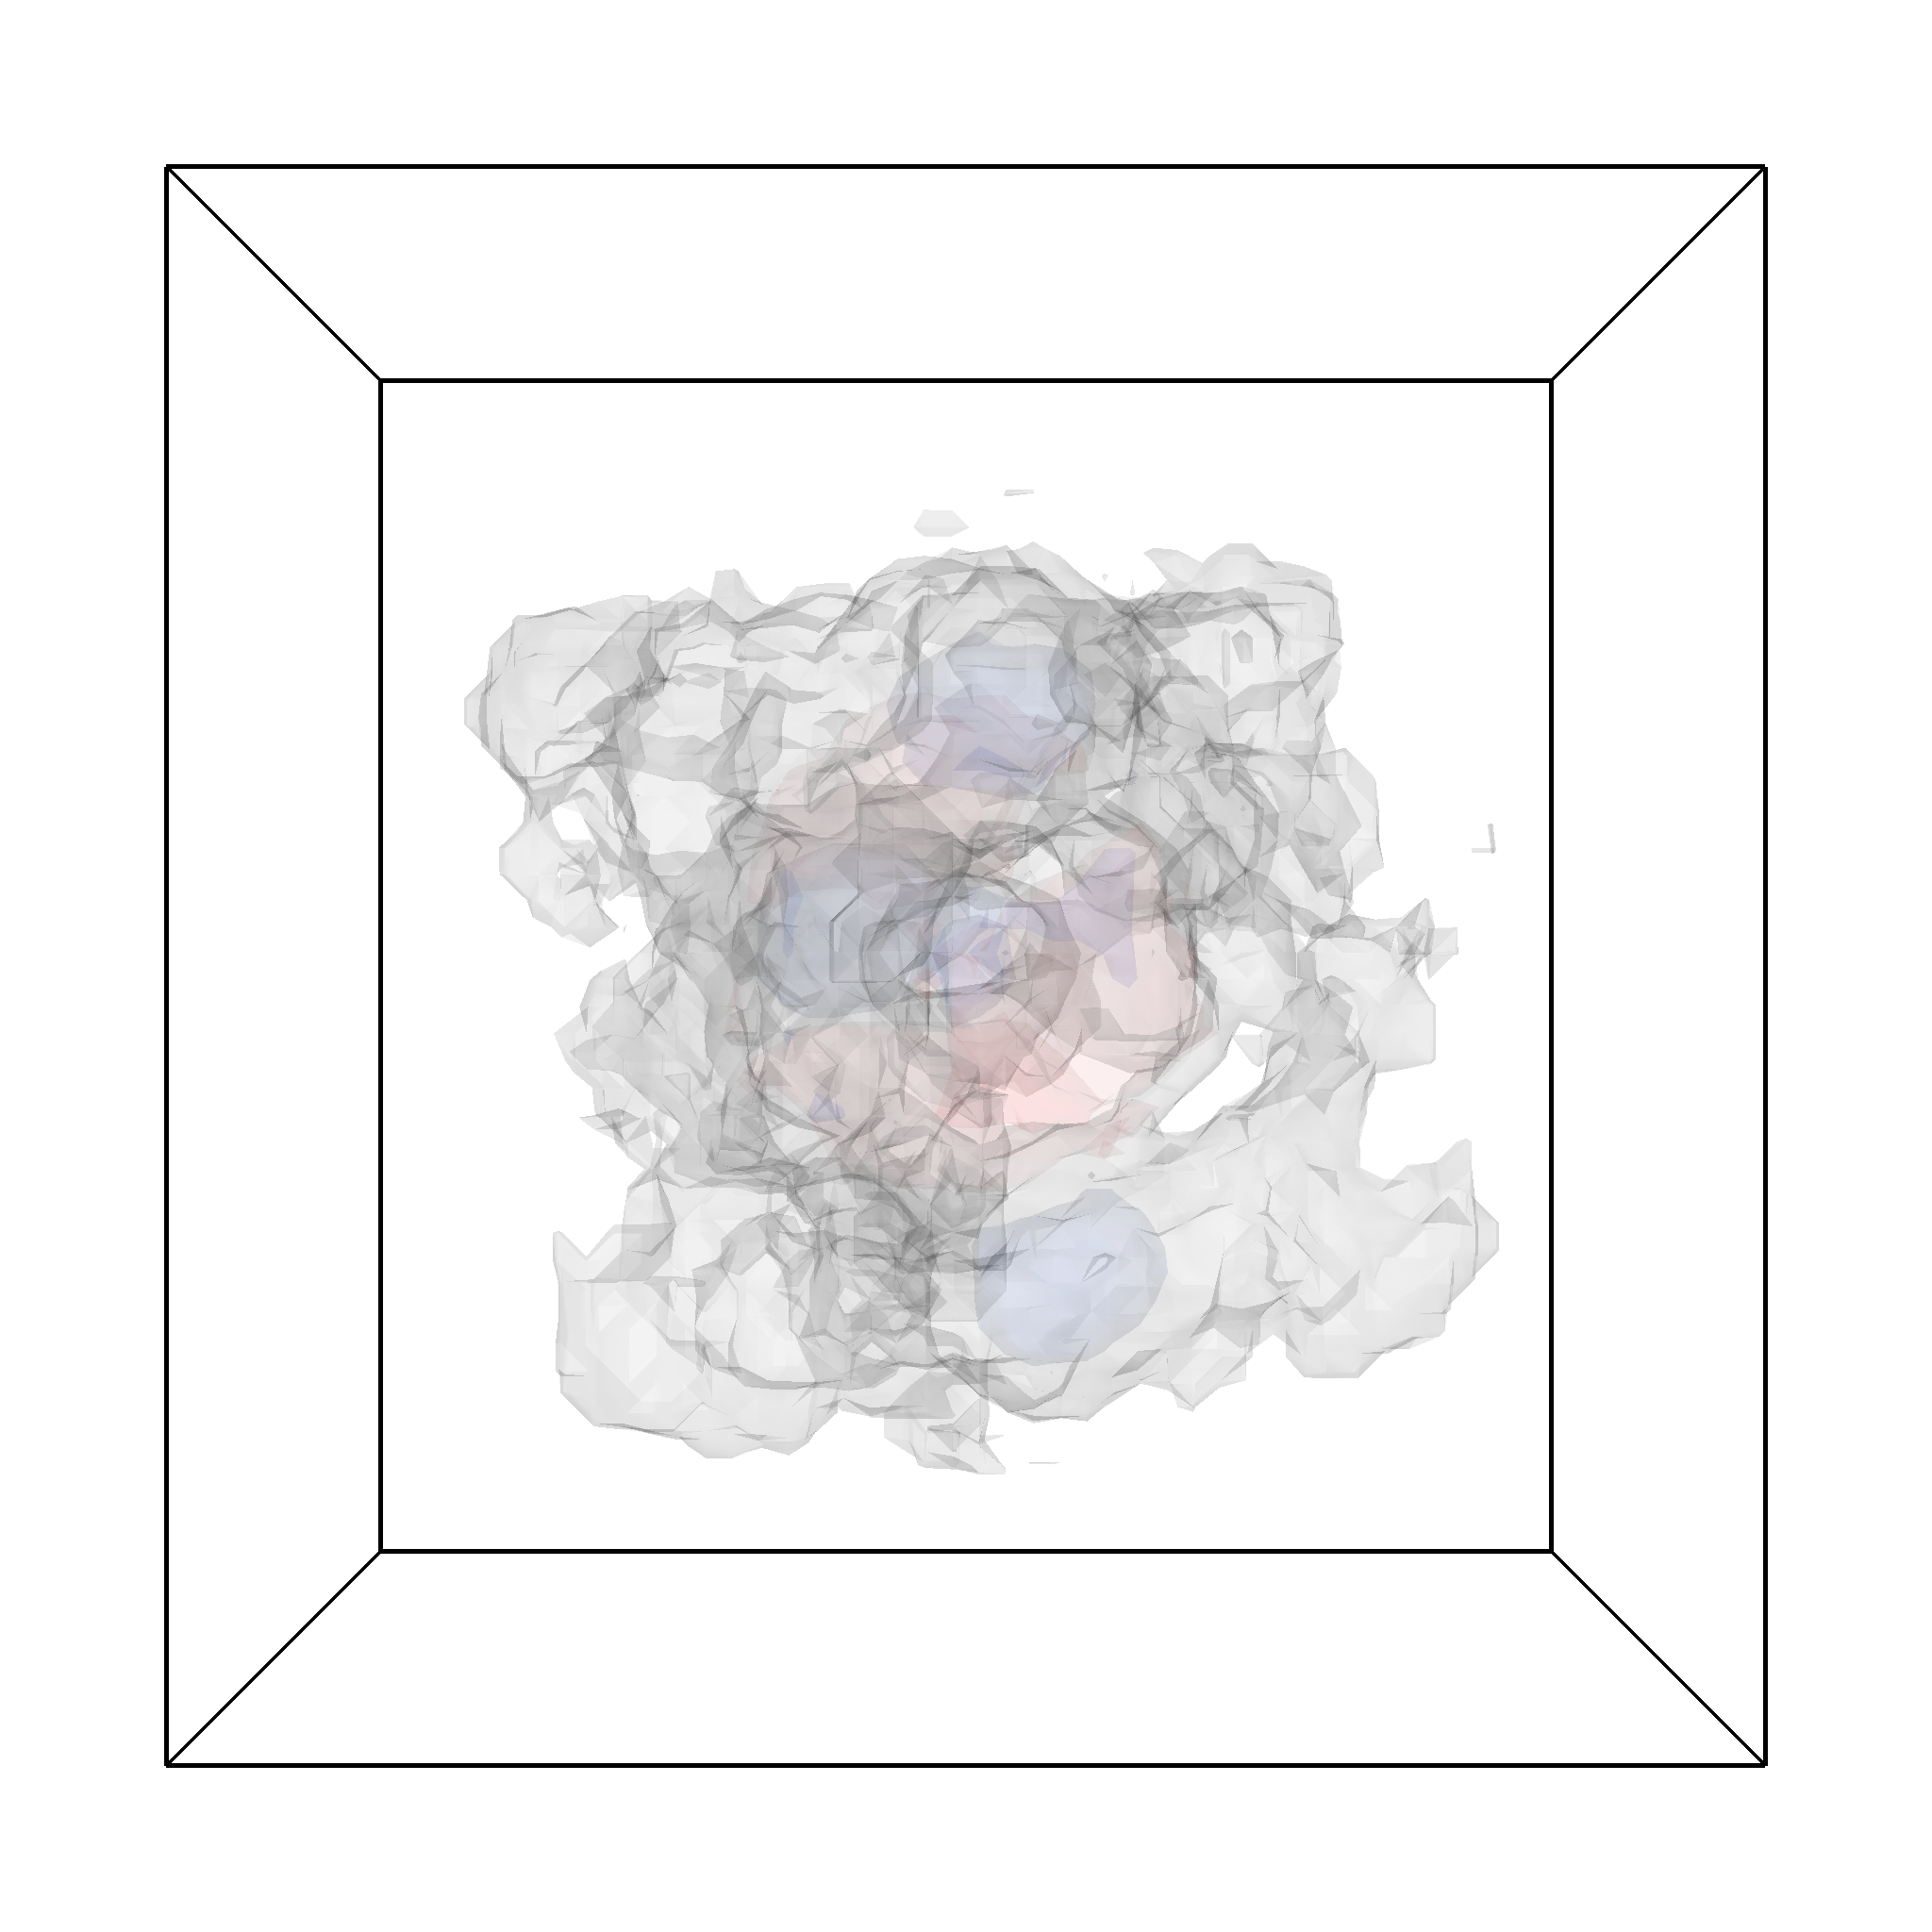
\includegraphics[width=0.272\columnwidth]{eigencage3.png}}
	\subfloat[][$\mathbf{v}_4$]{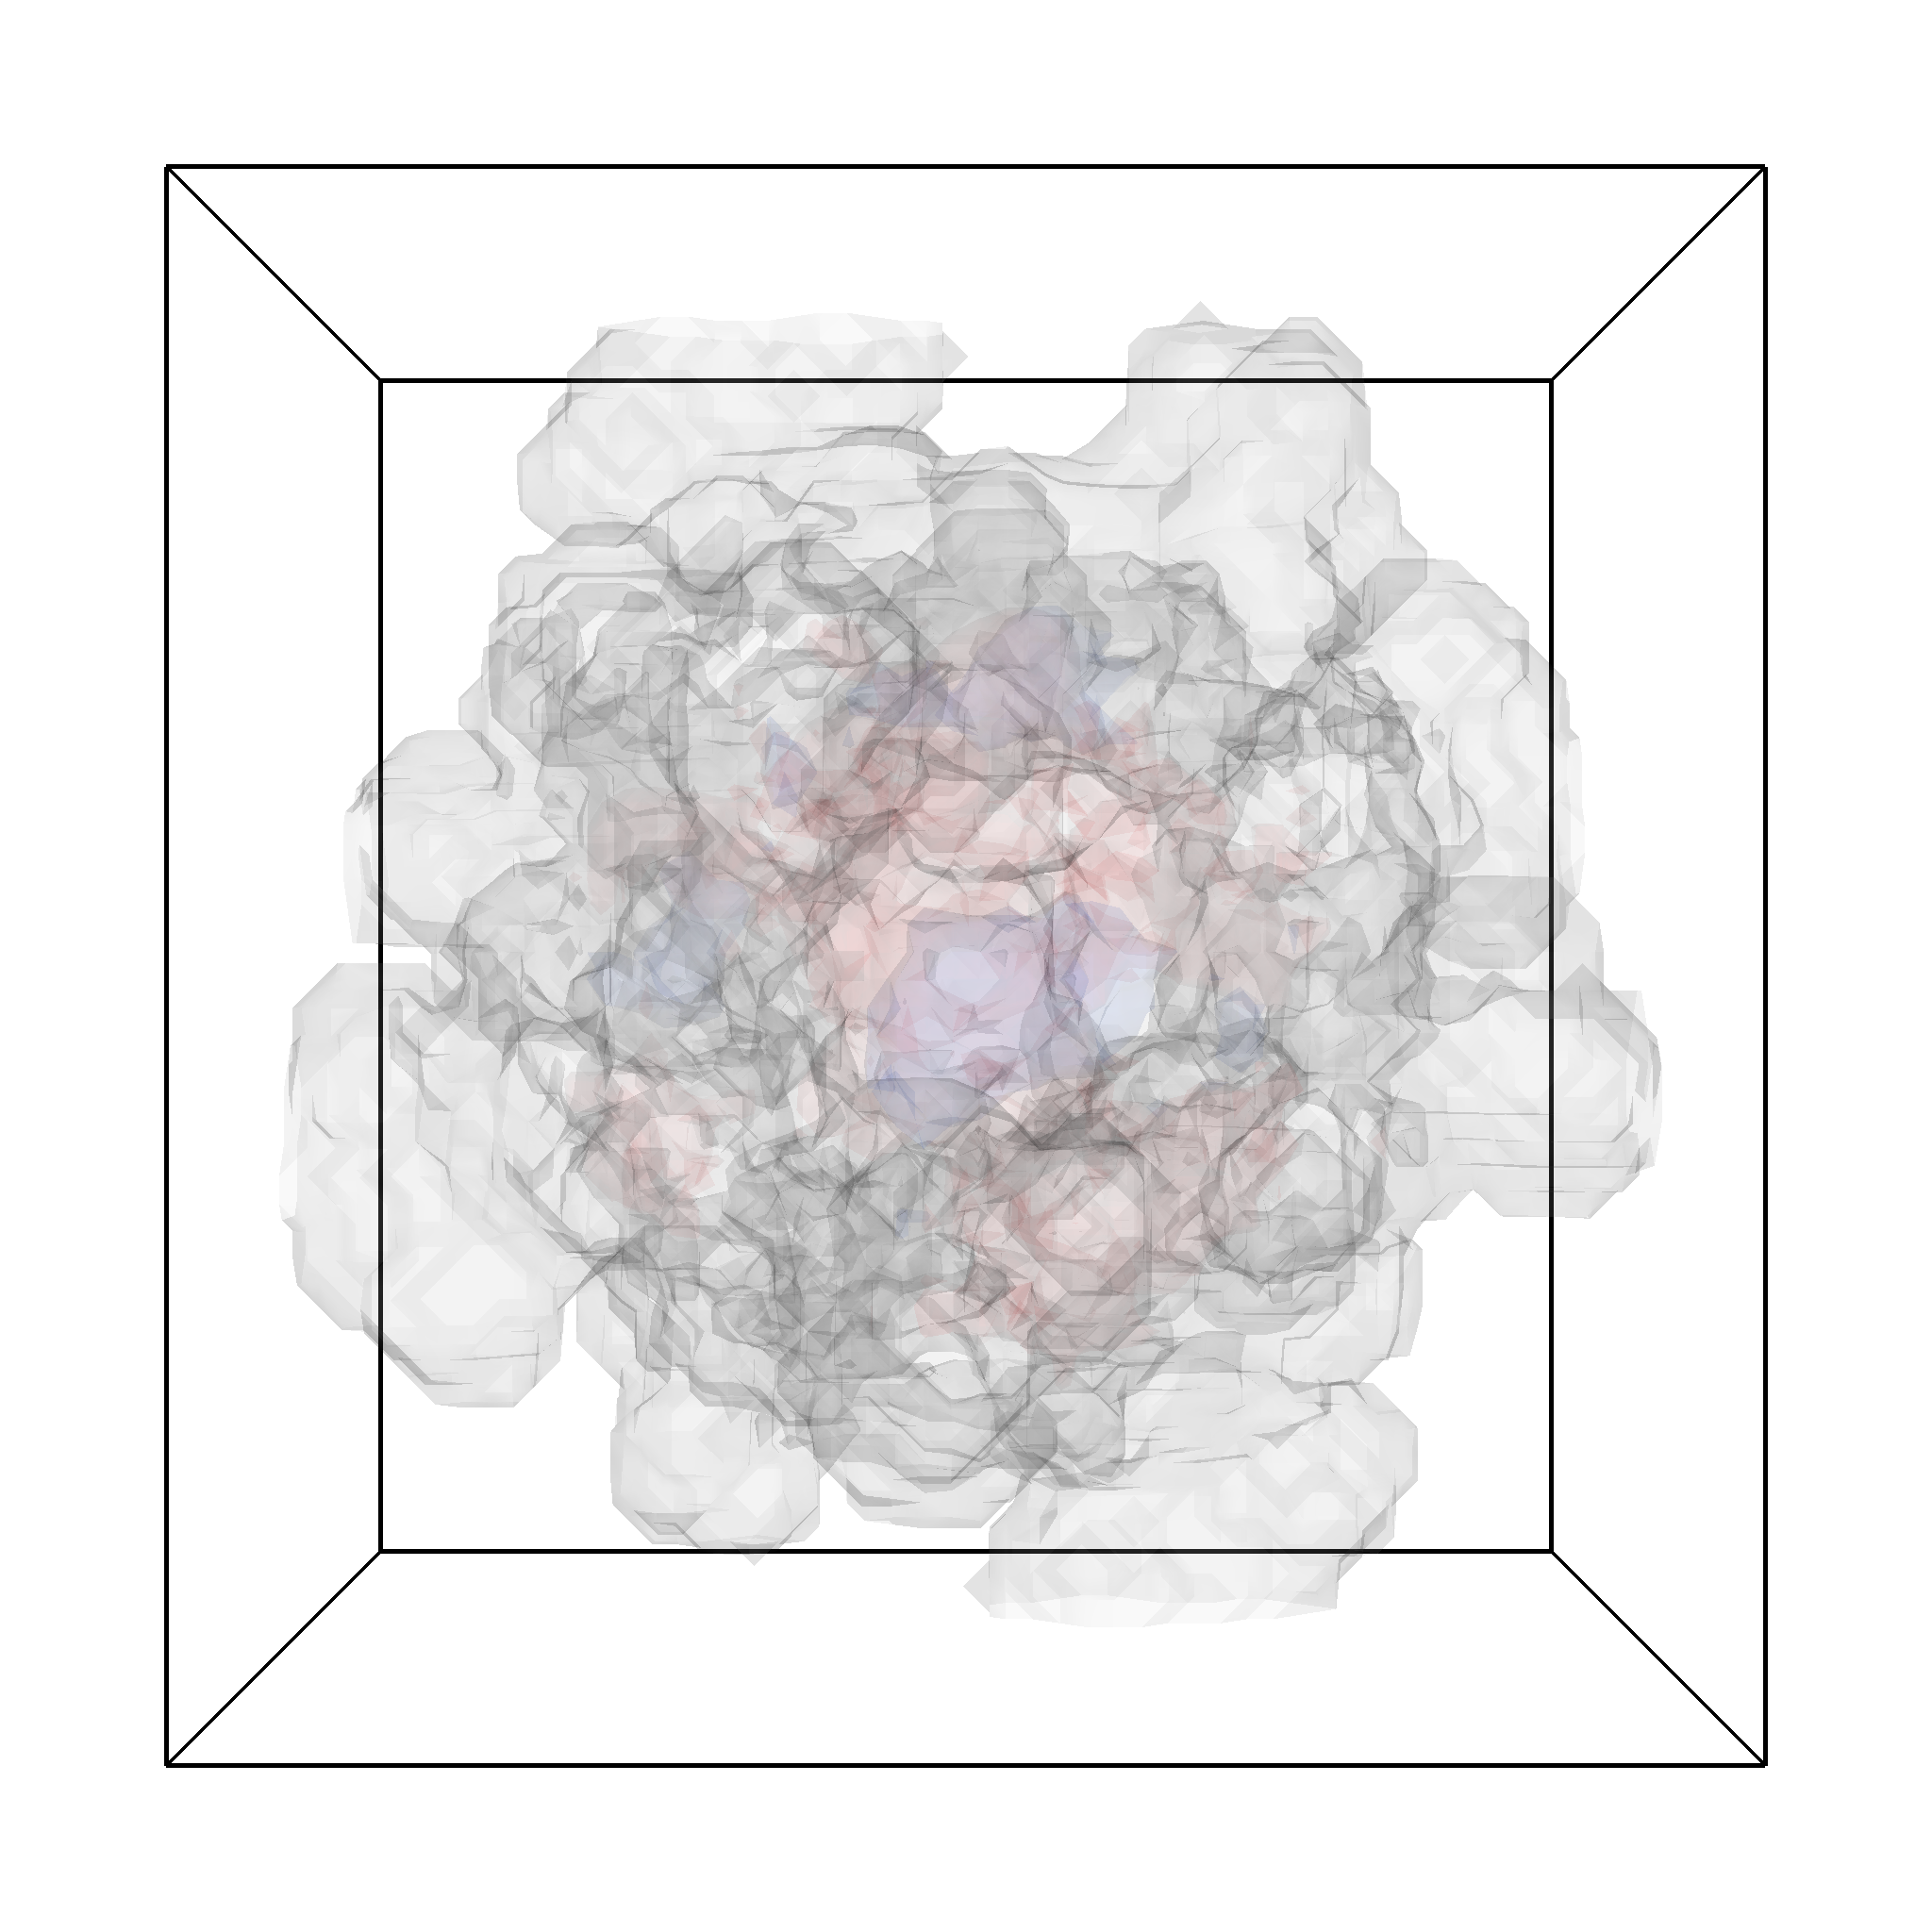
\includegraphics[width=0.272\columnwidth]{eigencage4.png}}
		\qquad
	\subfloat[][$\mathbf{v}_5$]{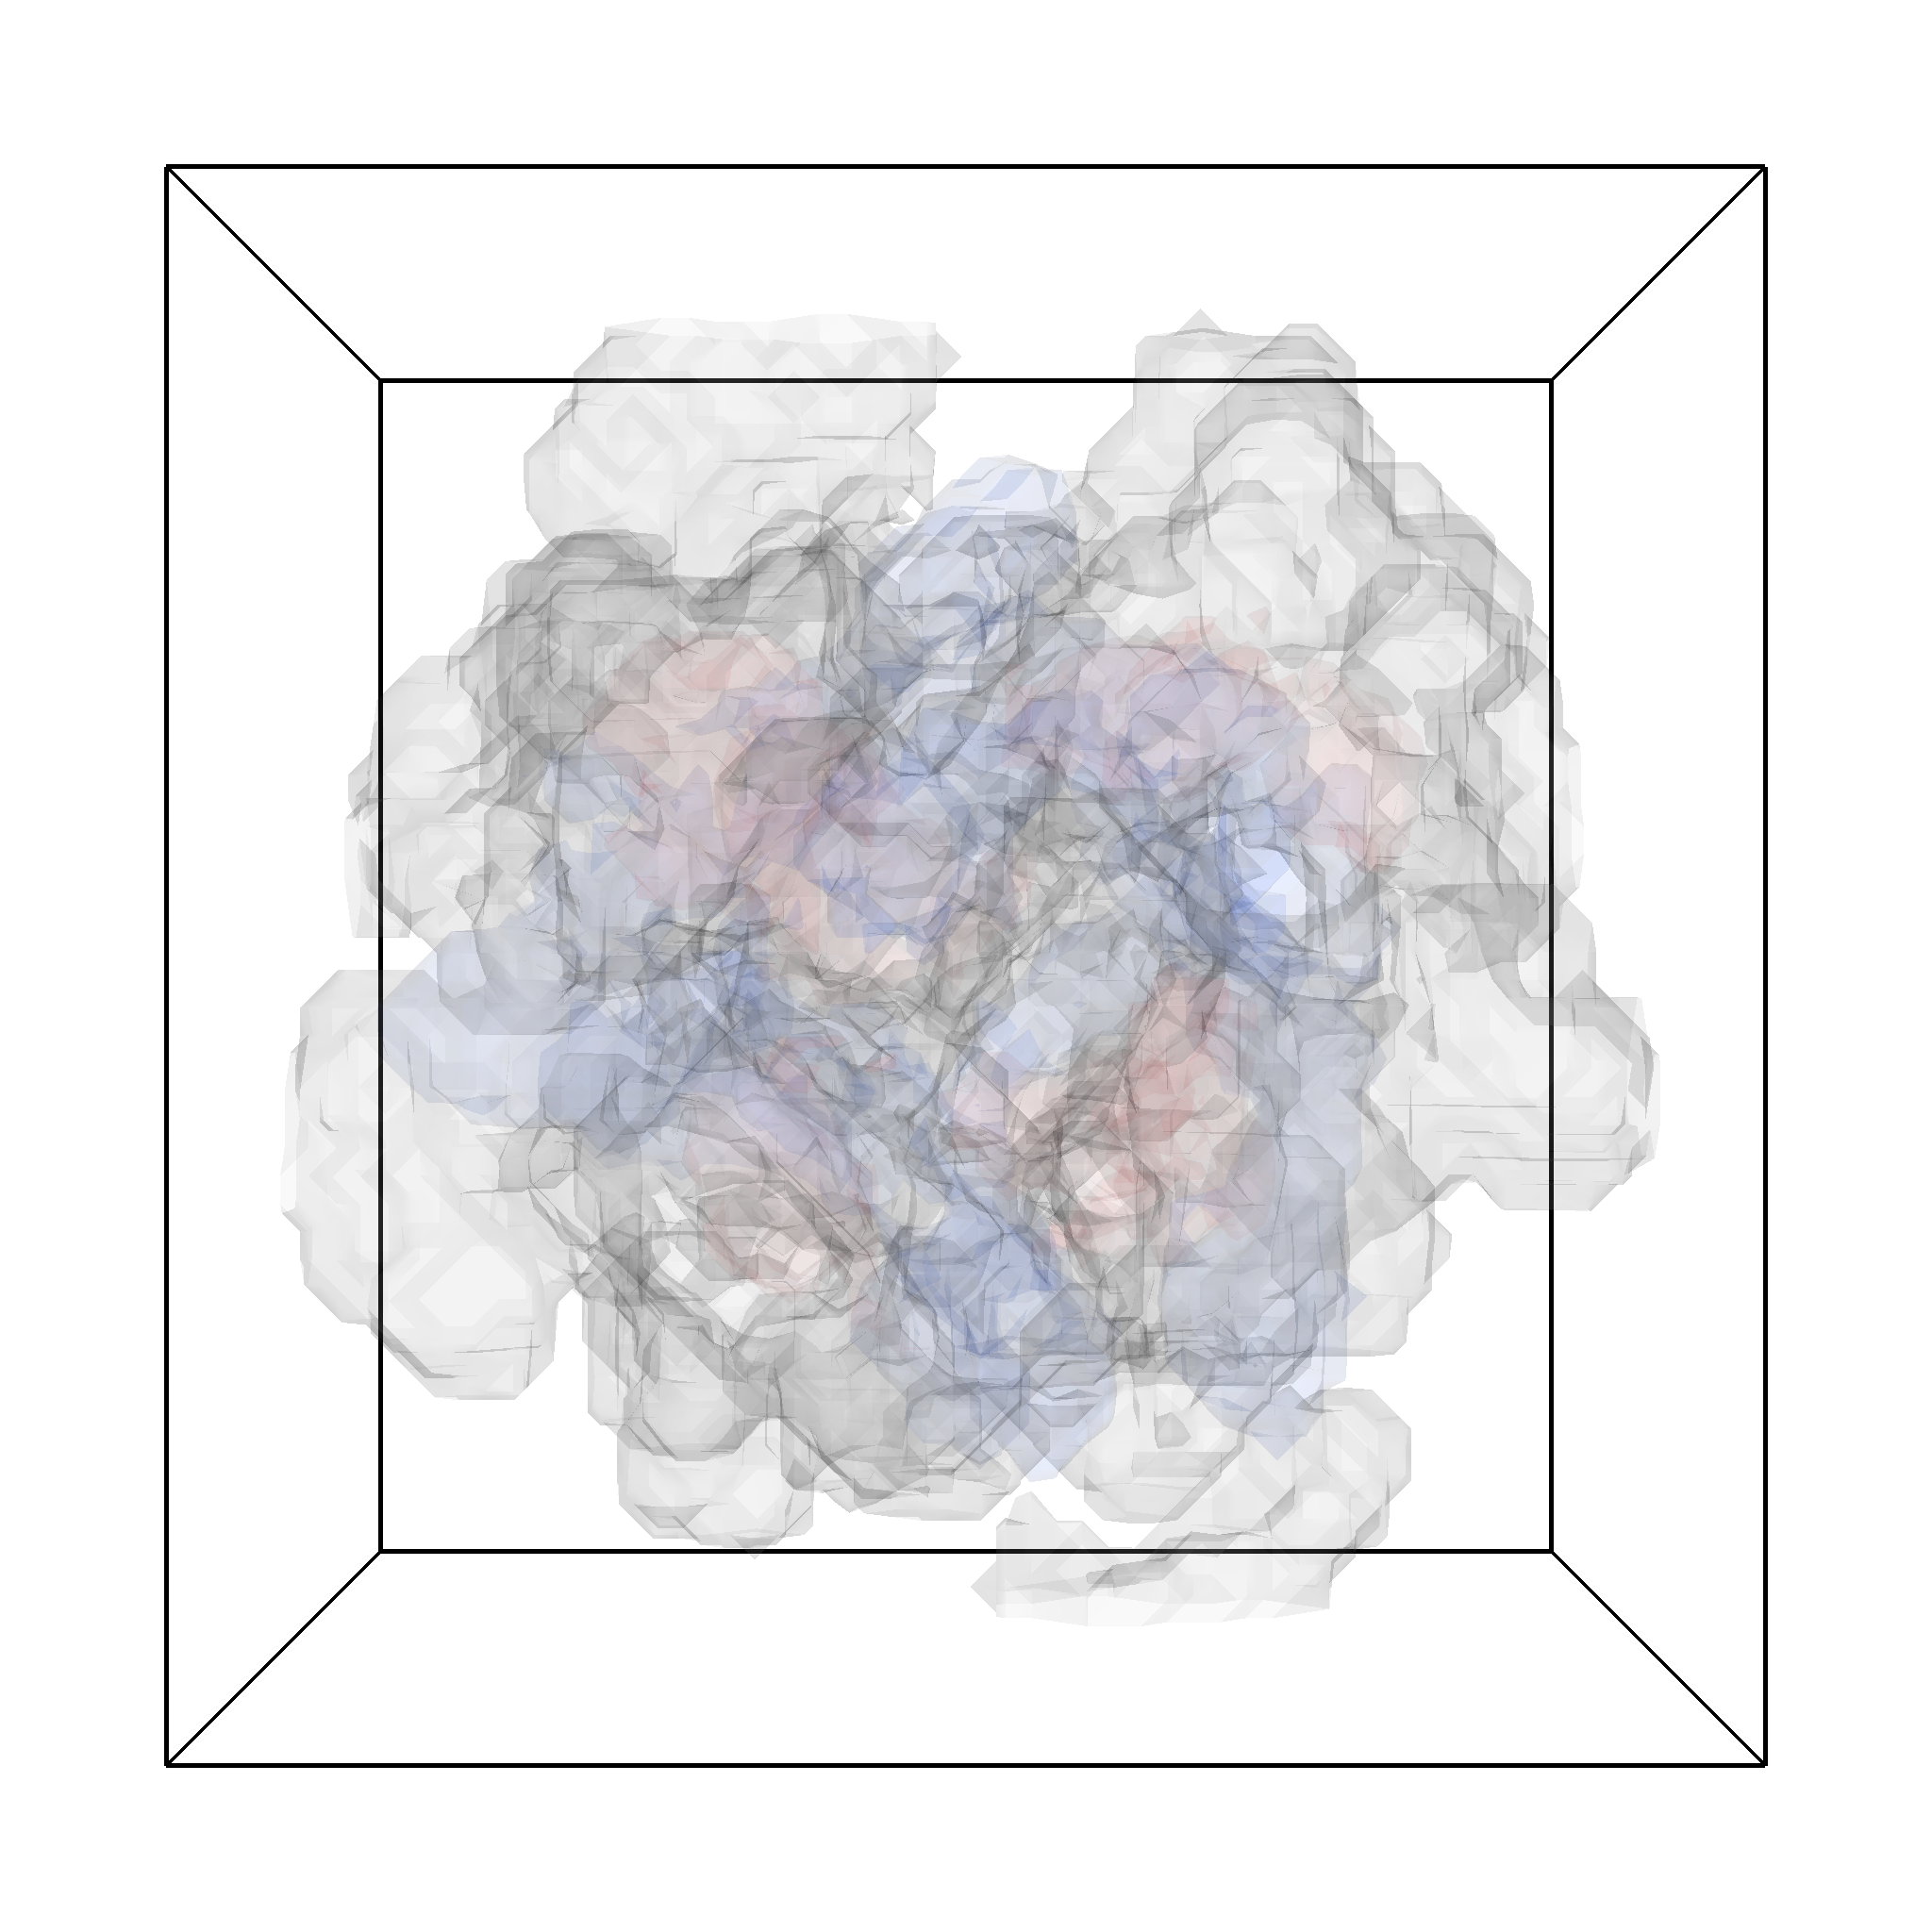
\includegraphics[width=0.272\columnwidth]{eigencage5.png}}
	\subfloat[][$\mathbf{v}_6$]{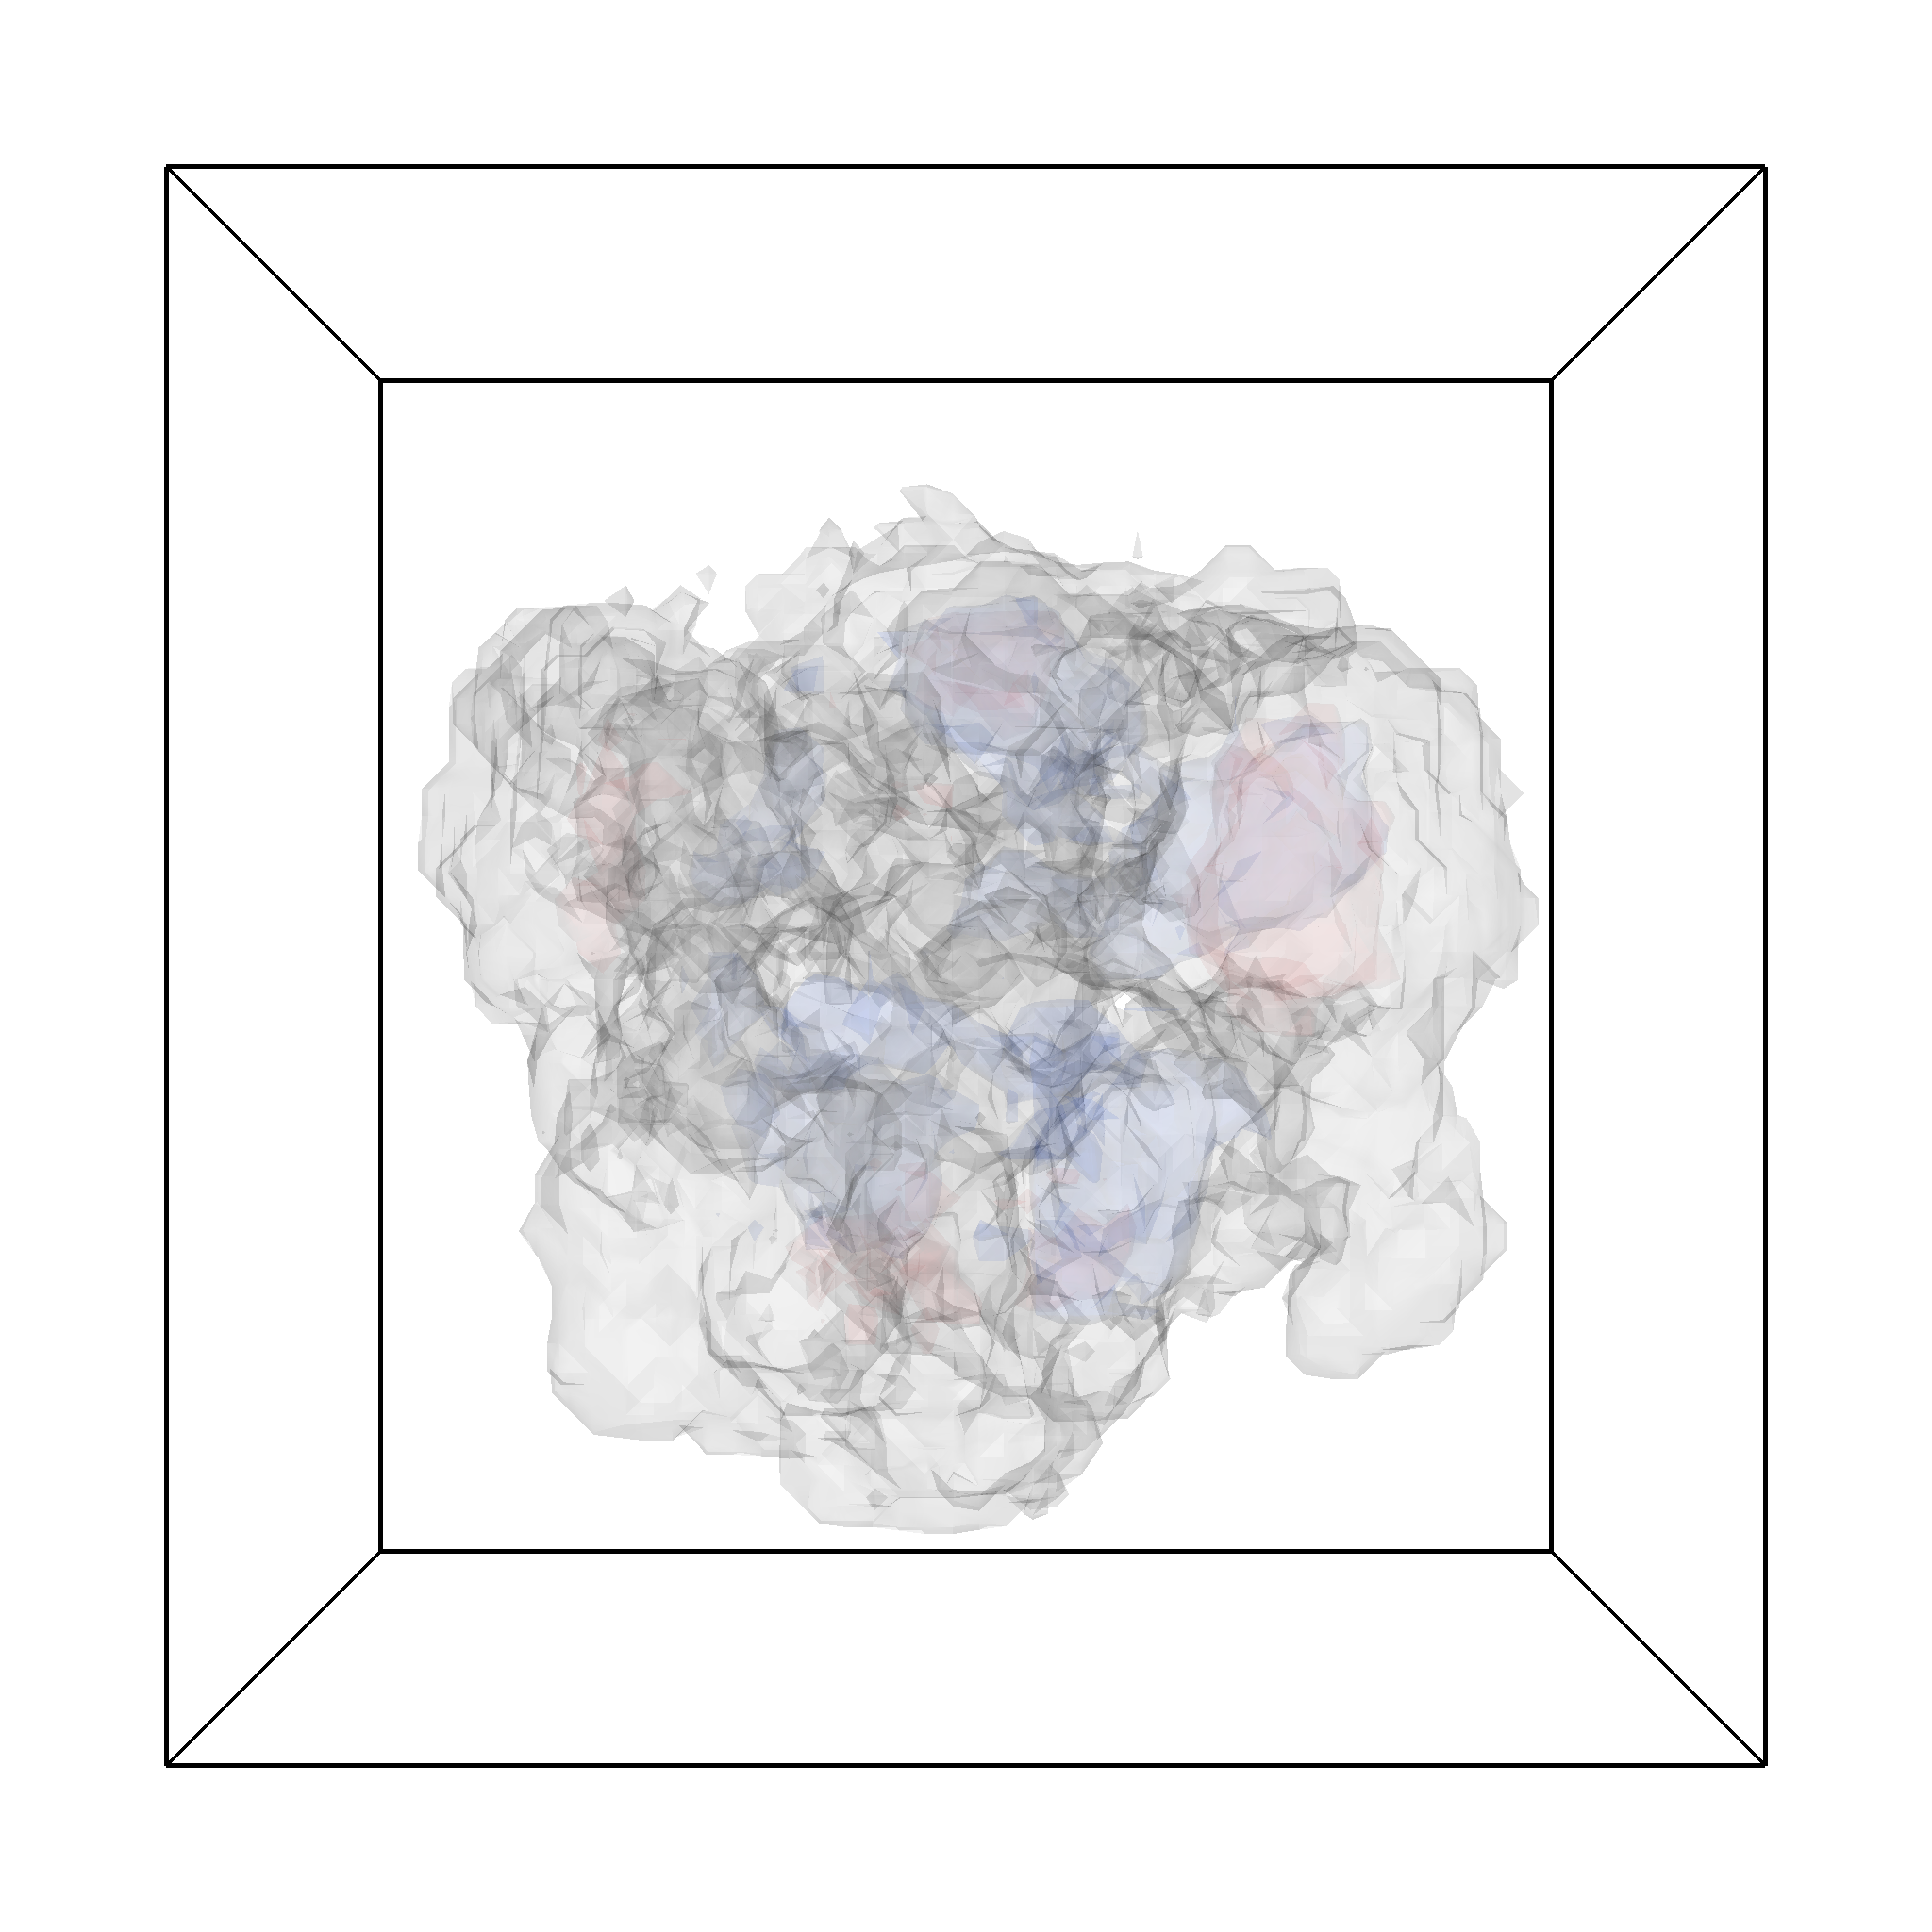
\includegraphics[width=0.272\columnwidth]{eigencage6.png}}
	\caption{Visualizing the eigencages. (a) Contour surfaces of the average 3D porosity image. {\color{red} Values increase from light to dark green.} (b-g) Contour surfaces of the first six eigencages. Blue: low (negative), Gray: intermediate, red: high (positive).
	} \label{fig:eigencages}
\end{figure}

\subsection{Reconstructing a cage from eigencages} From the view of SVD, each 3D porosity image is constructed from a linear combination of the eigencages (see eqn.~\ref{eq:latent_space_view}). We show here that, remarkably, even the six eigencages in Fig.~\ref{fig:eigencages} can be enough to visually reproduce the structure of the cavity in a porous organic cage molecule. As an example, in Fig.~\ref{fig:cage_reconstruction} we show the approximated reconstruction of the 3D porosity image of porous organic cage molecule \textbf{B25} using different numbers of eigencages. Mathematically, Fig.~\ref{fig:cage_reconstruction} shows the approximant given by eqn.~\ref{eq:latent_space_view} with $\nu=1,2,...,9$. Expressing \textbf{B25} in terms of the first two eigencages is insufficient to capture its shape; for $\nu=4$, the cavity and windows of \textbf{B25} are captured to some extent. Only until we reach $\nu=6$ does the outer-contour of the reconstructed 3D void space image of \textbf{B25} well-approximate the shape of the molecule. The reconstructed \textbf{B25} 3D porosity image with $\nu=9$ is approaching visual indistinguishably from the exact 3D void space image in Fig.~\ref{fig:b25_exact}. This shows that e.g. a $\nu=9$-dimensional latent representation of \textbf{B25} contains sufficient information to visually reproduce the shape of its cavity.

\begin{figure}
% made with image zoom 1.4. see saved VisIT session in data/grids. mesh width 4, see snapshot.vtk
\centering
	\subfloat[][\textbf{B25}, exact $\nu=74$]{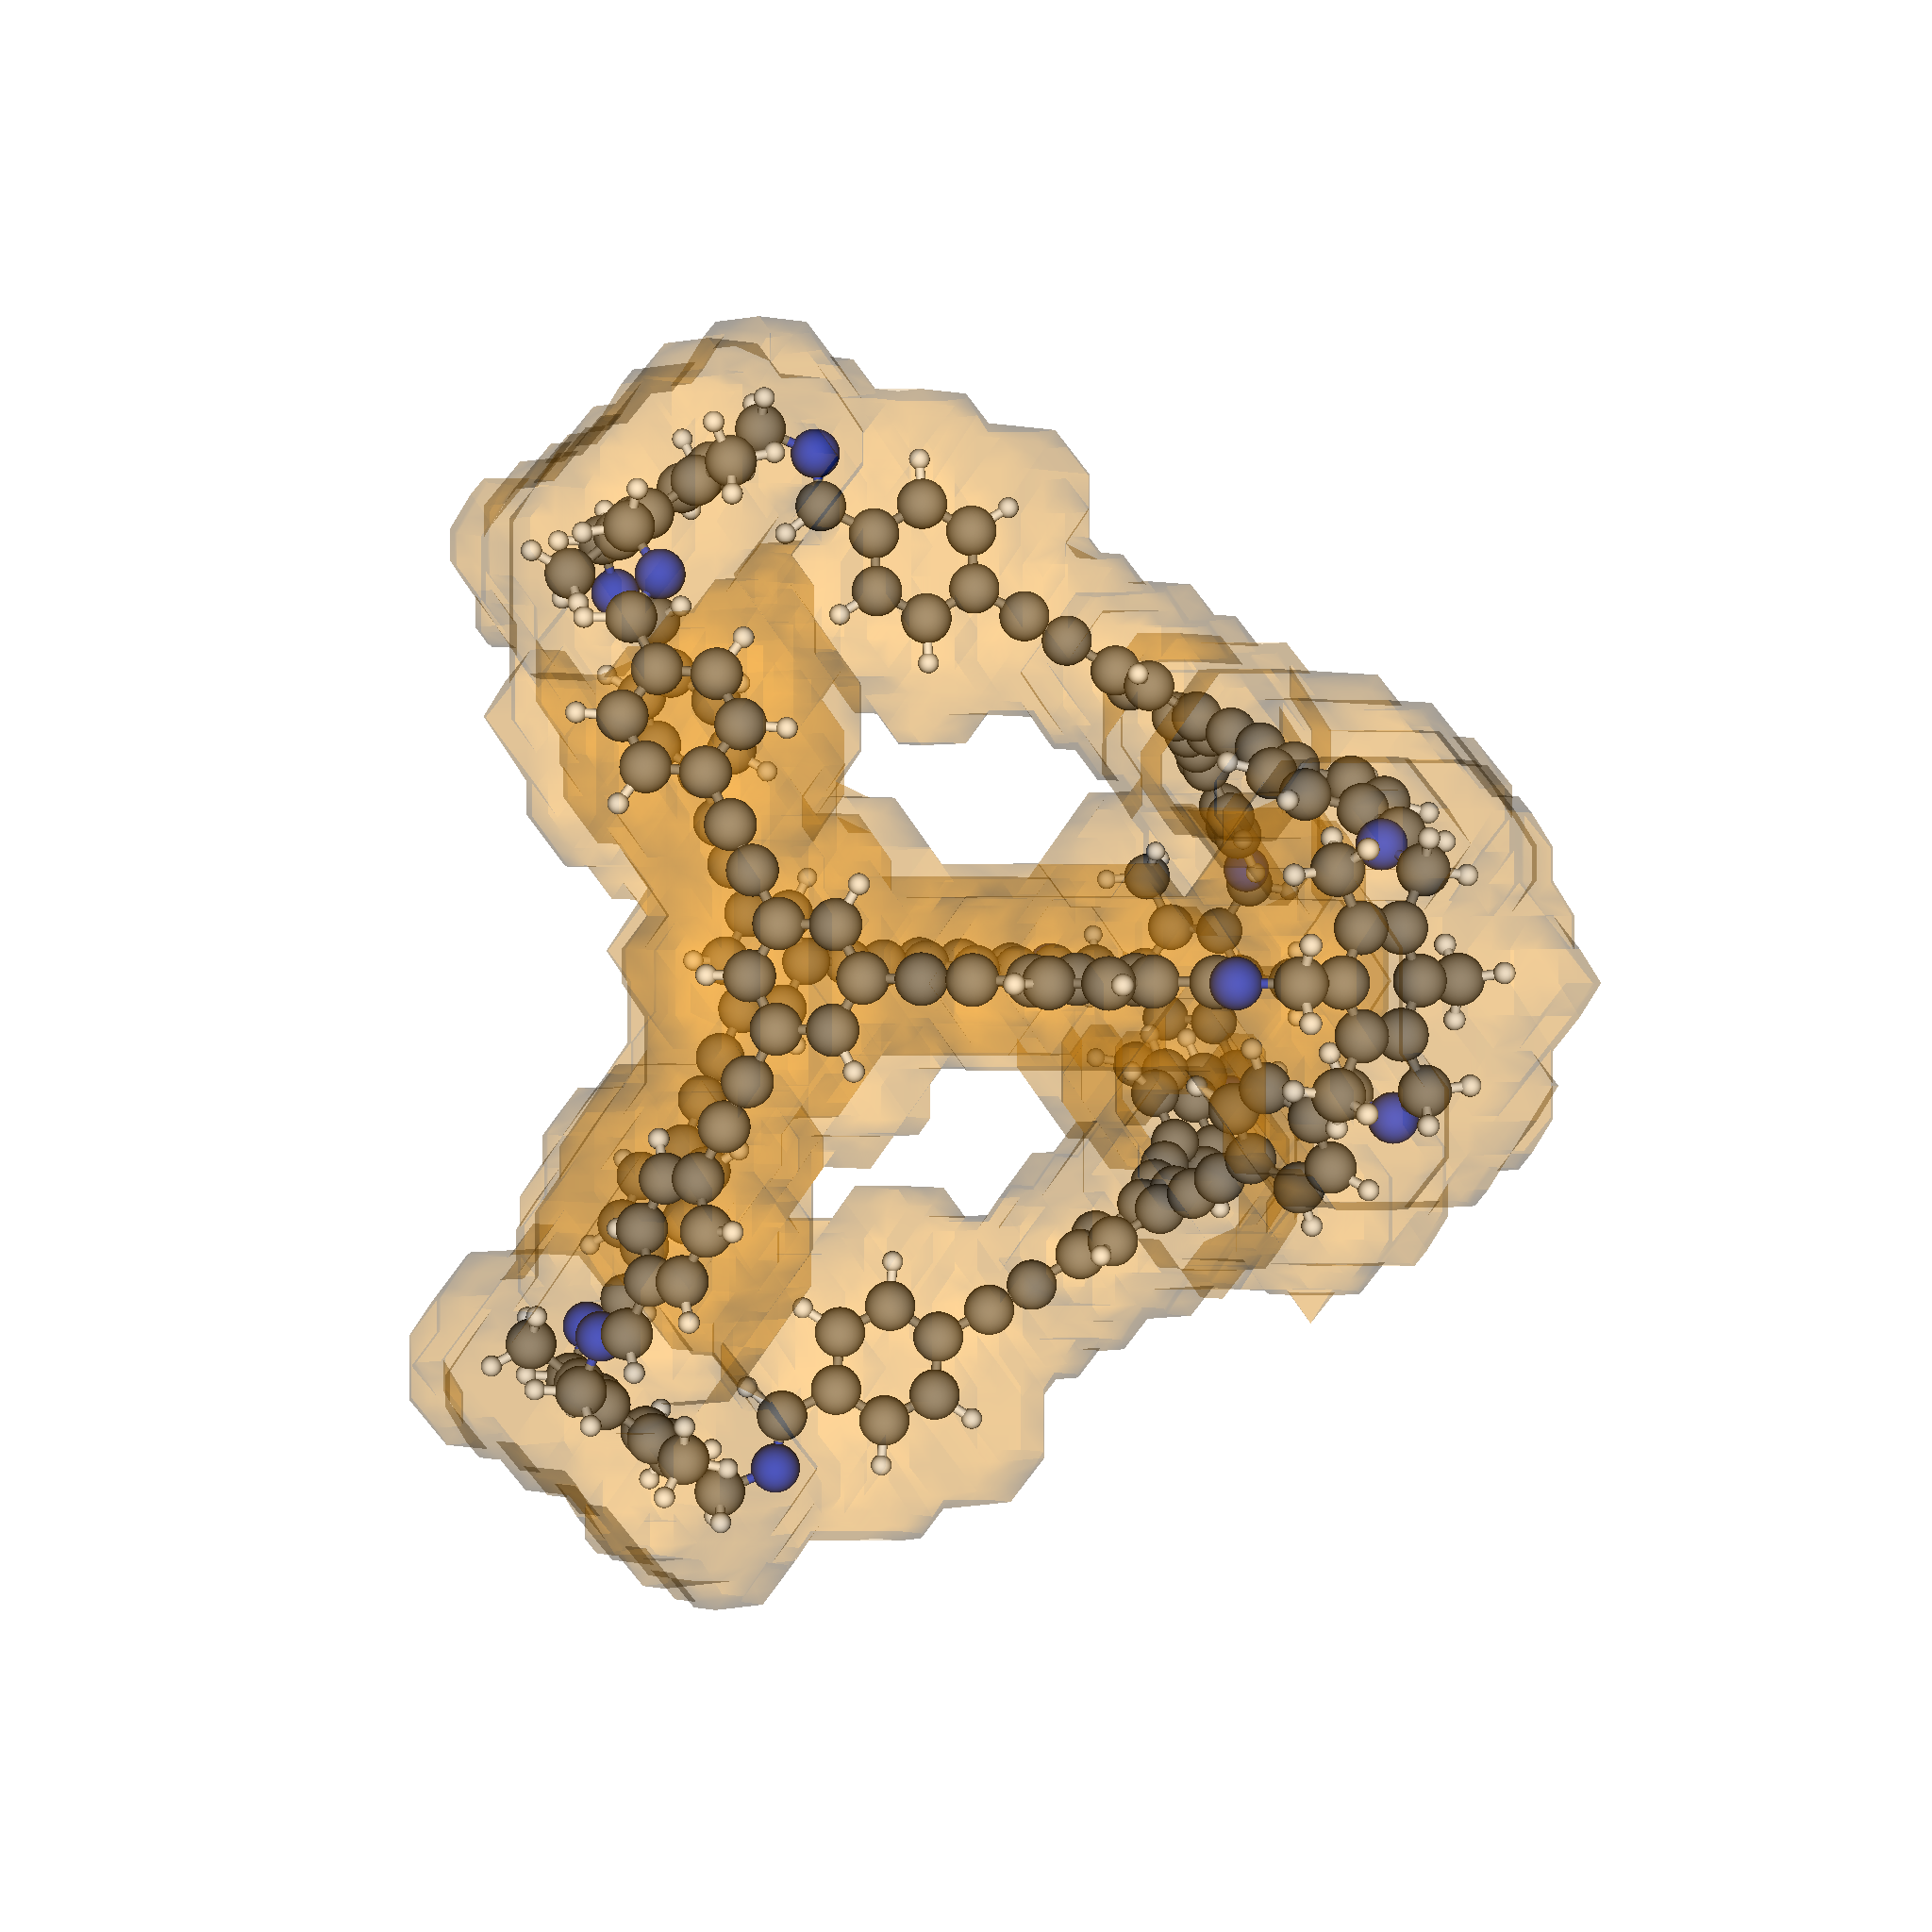
\includegraphics[width=0.275\columnwidth]{B25_raw.png} \label{fig:b25_exact}}
	\qquad
	\subfloat[][$\nu=1$]{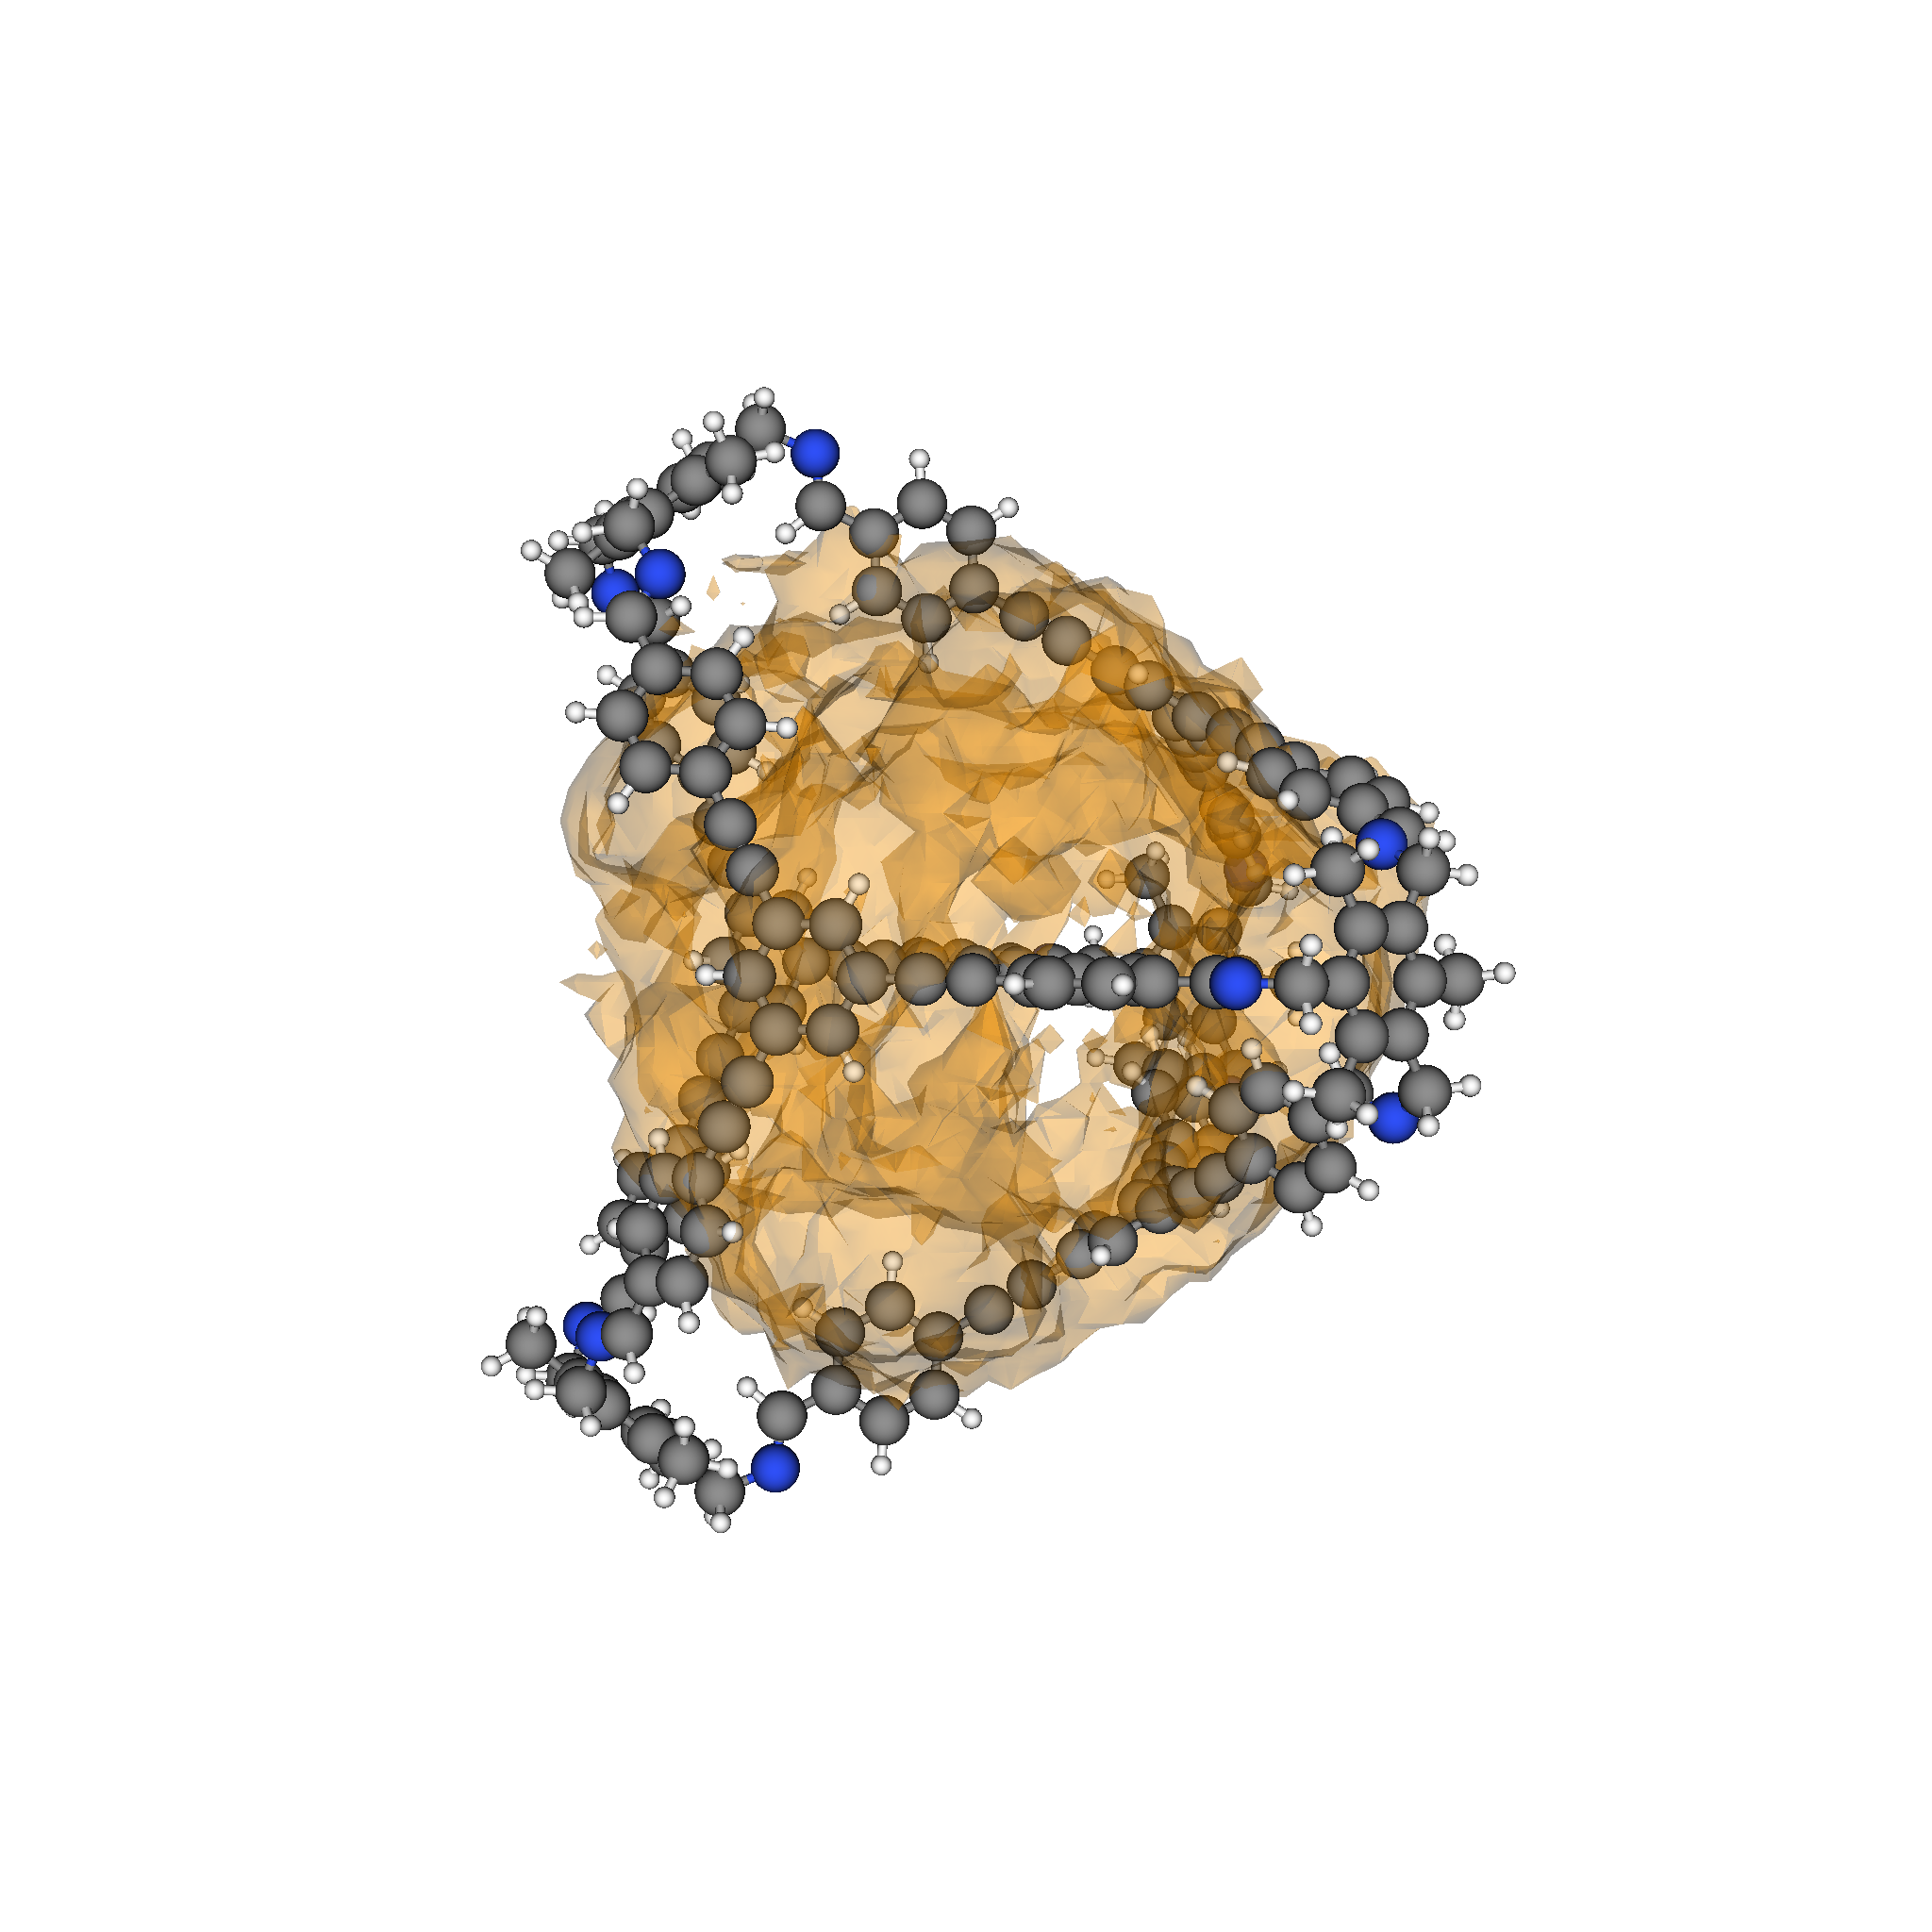
\includegraphics[width=0.275\columnwidth]{B25_nu1.png}}
	\subfloat[][$\nu=2$]{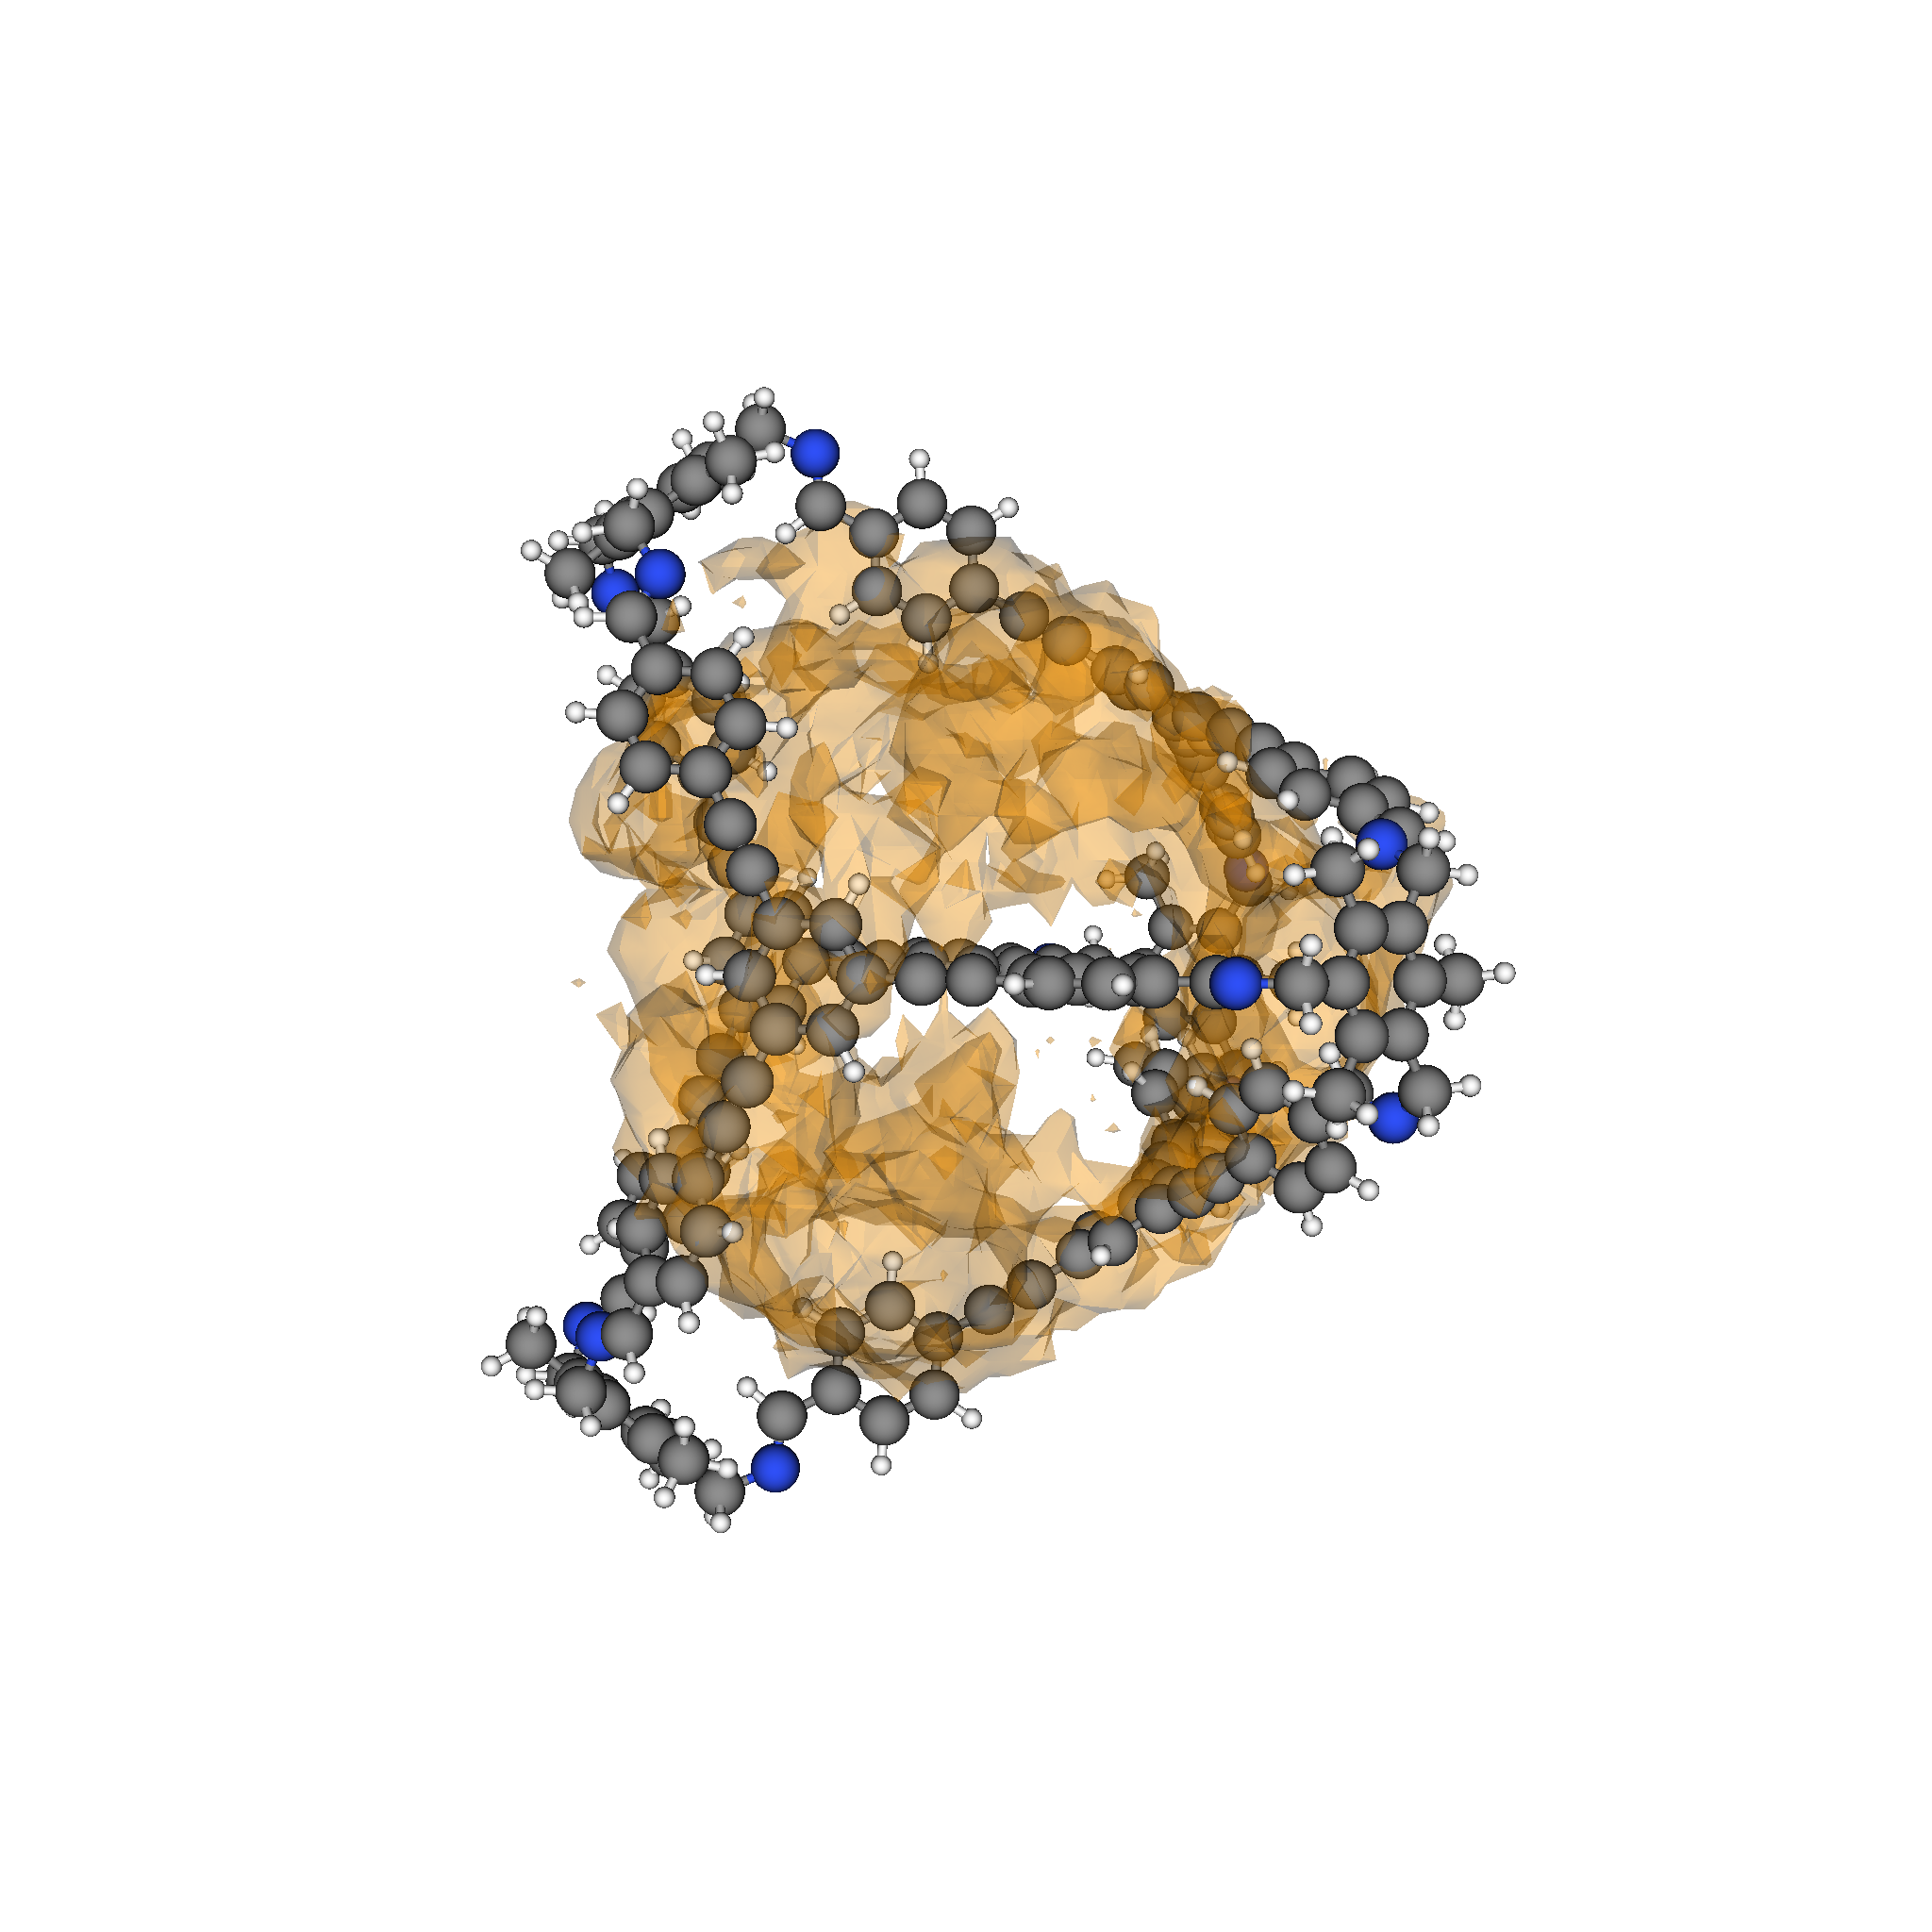
\includegraphics[width=0.275\columnwidth]{B25_nu2.png}}
	\subfloat[][$\nu=3$]{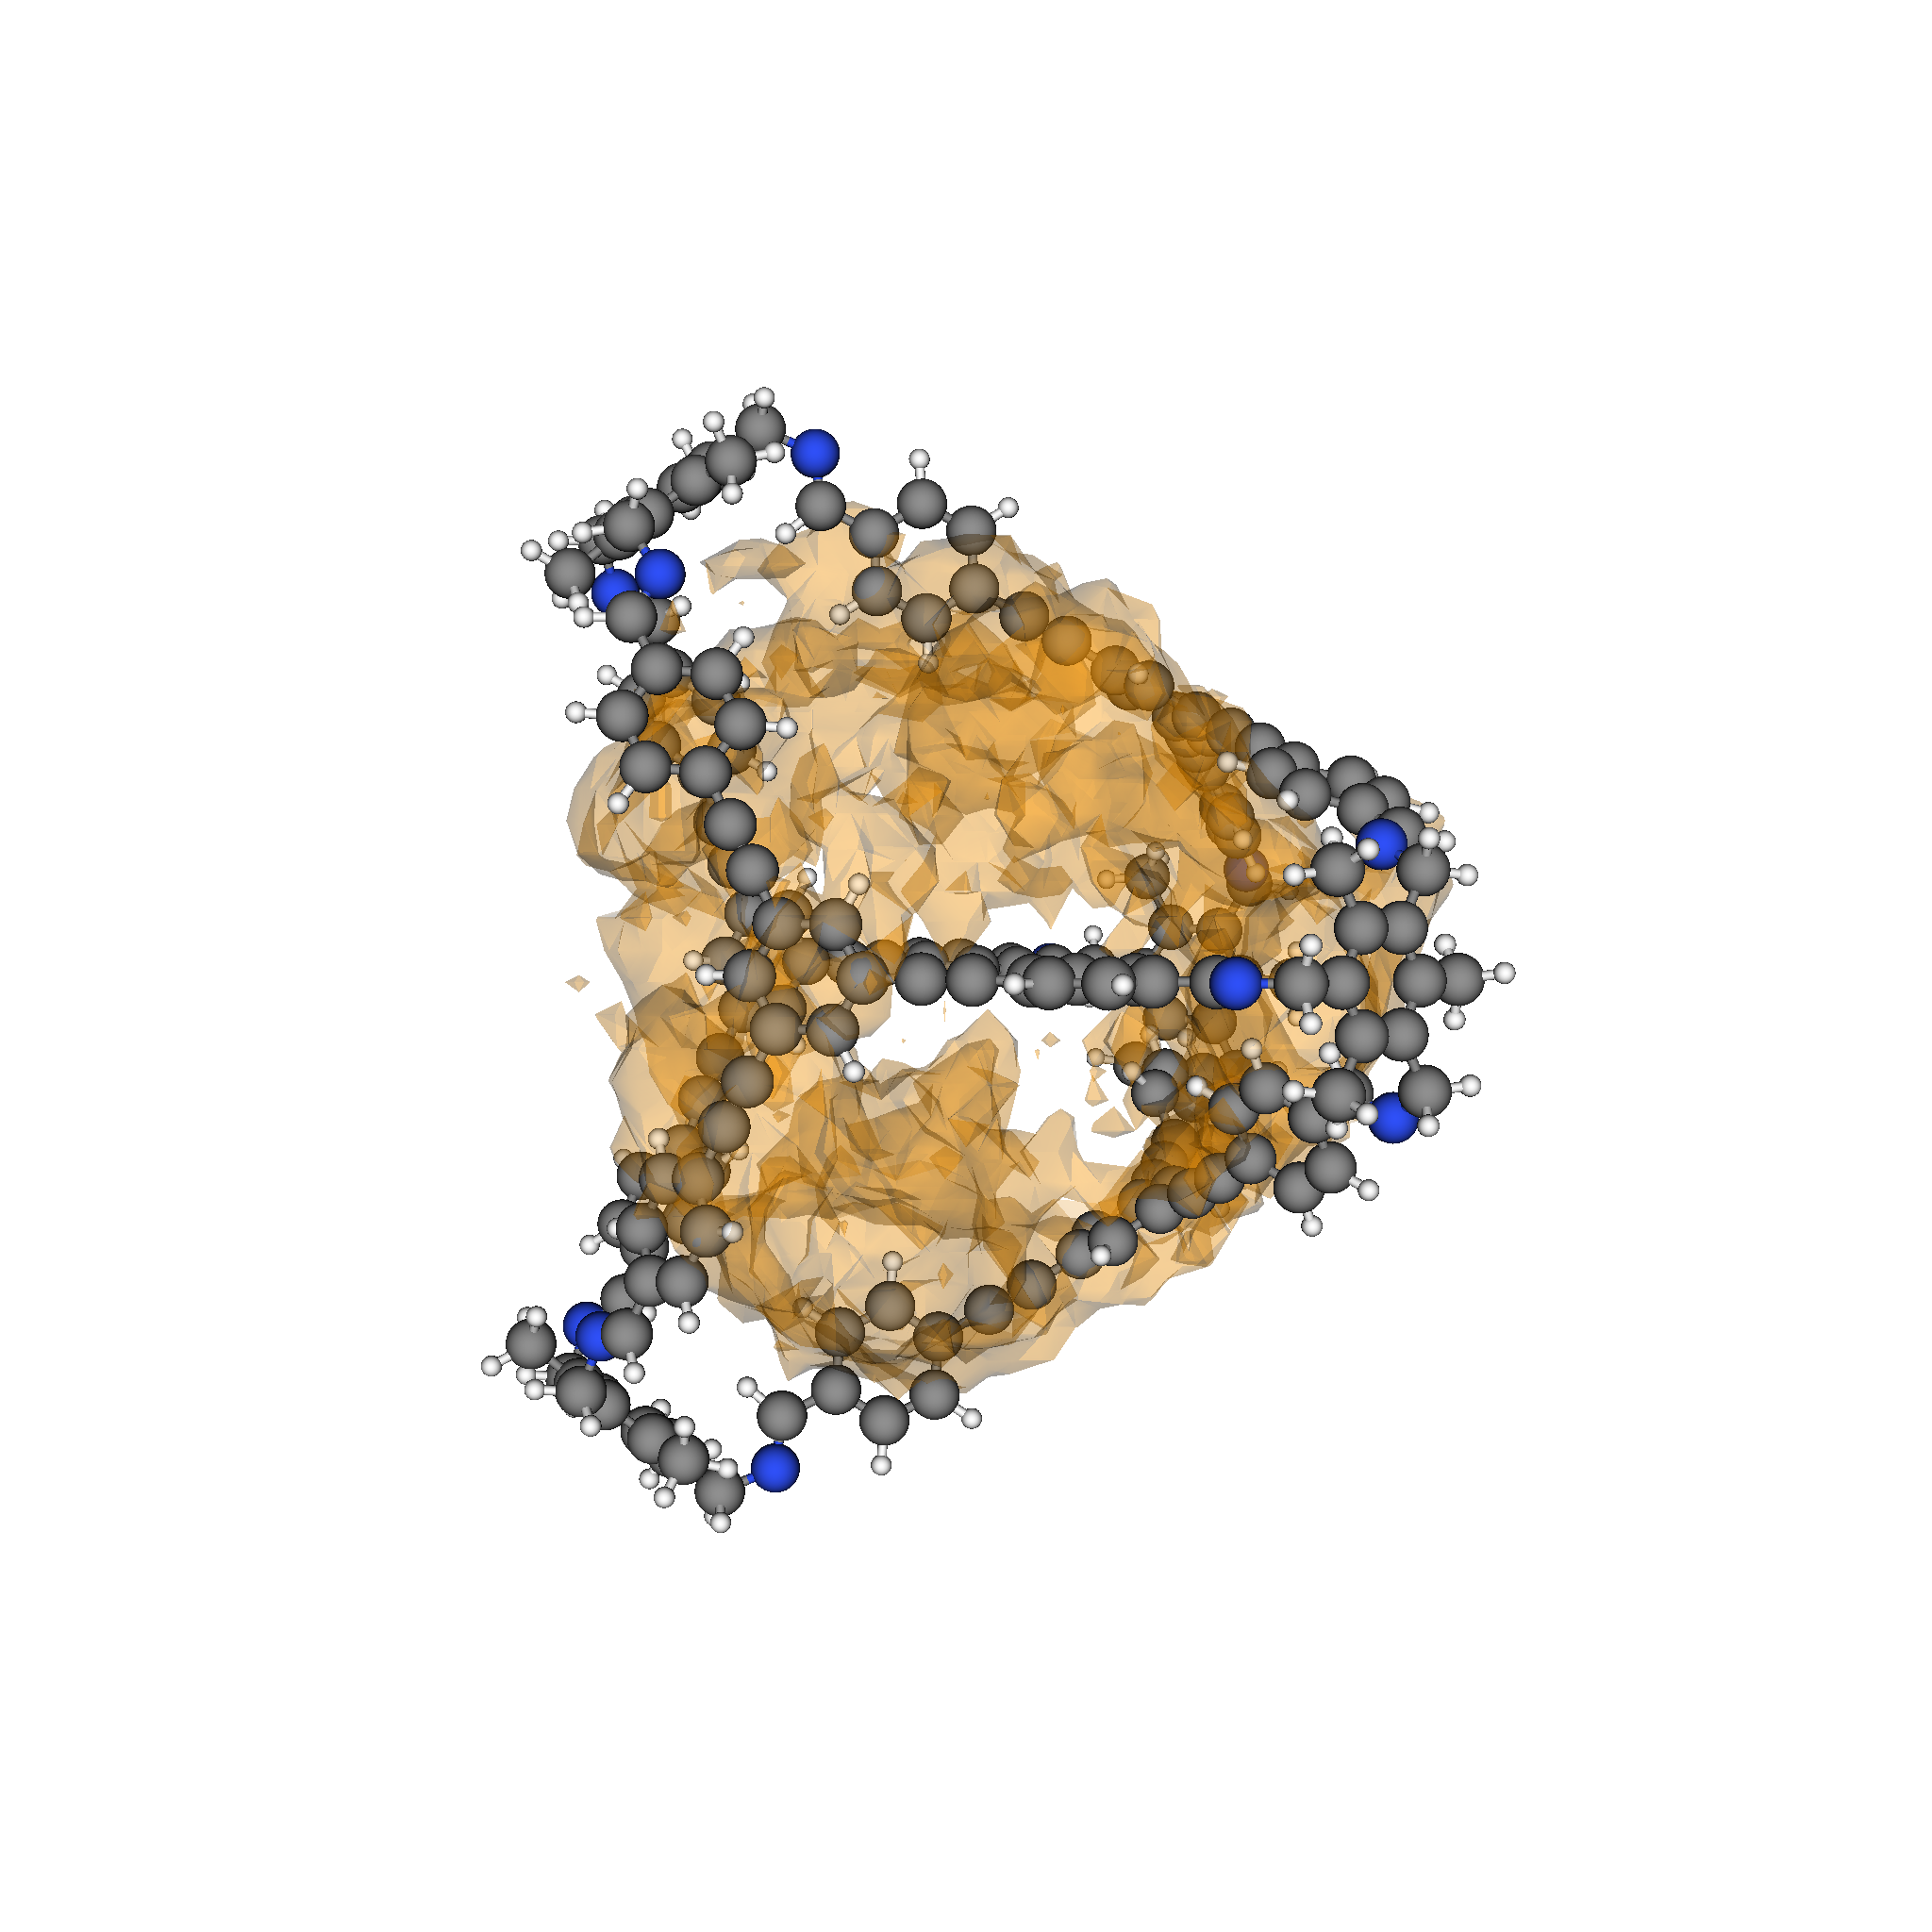
\includegraphics[width=0.275\columnwidth]{B25_nu3.png}}
	\qquad
	\subfloat[][$\nu=4$]{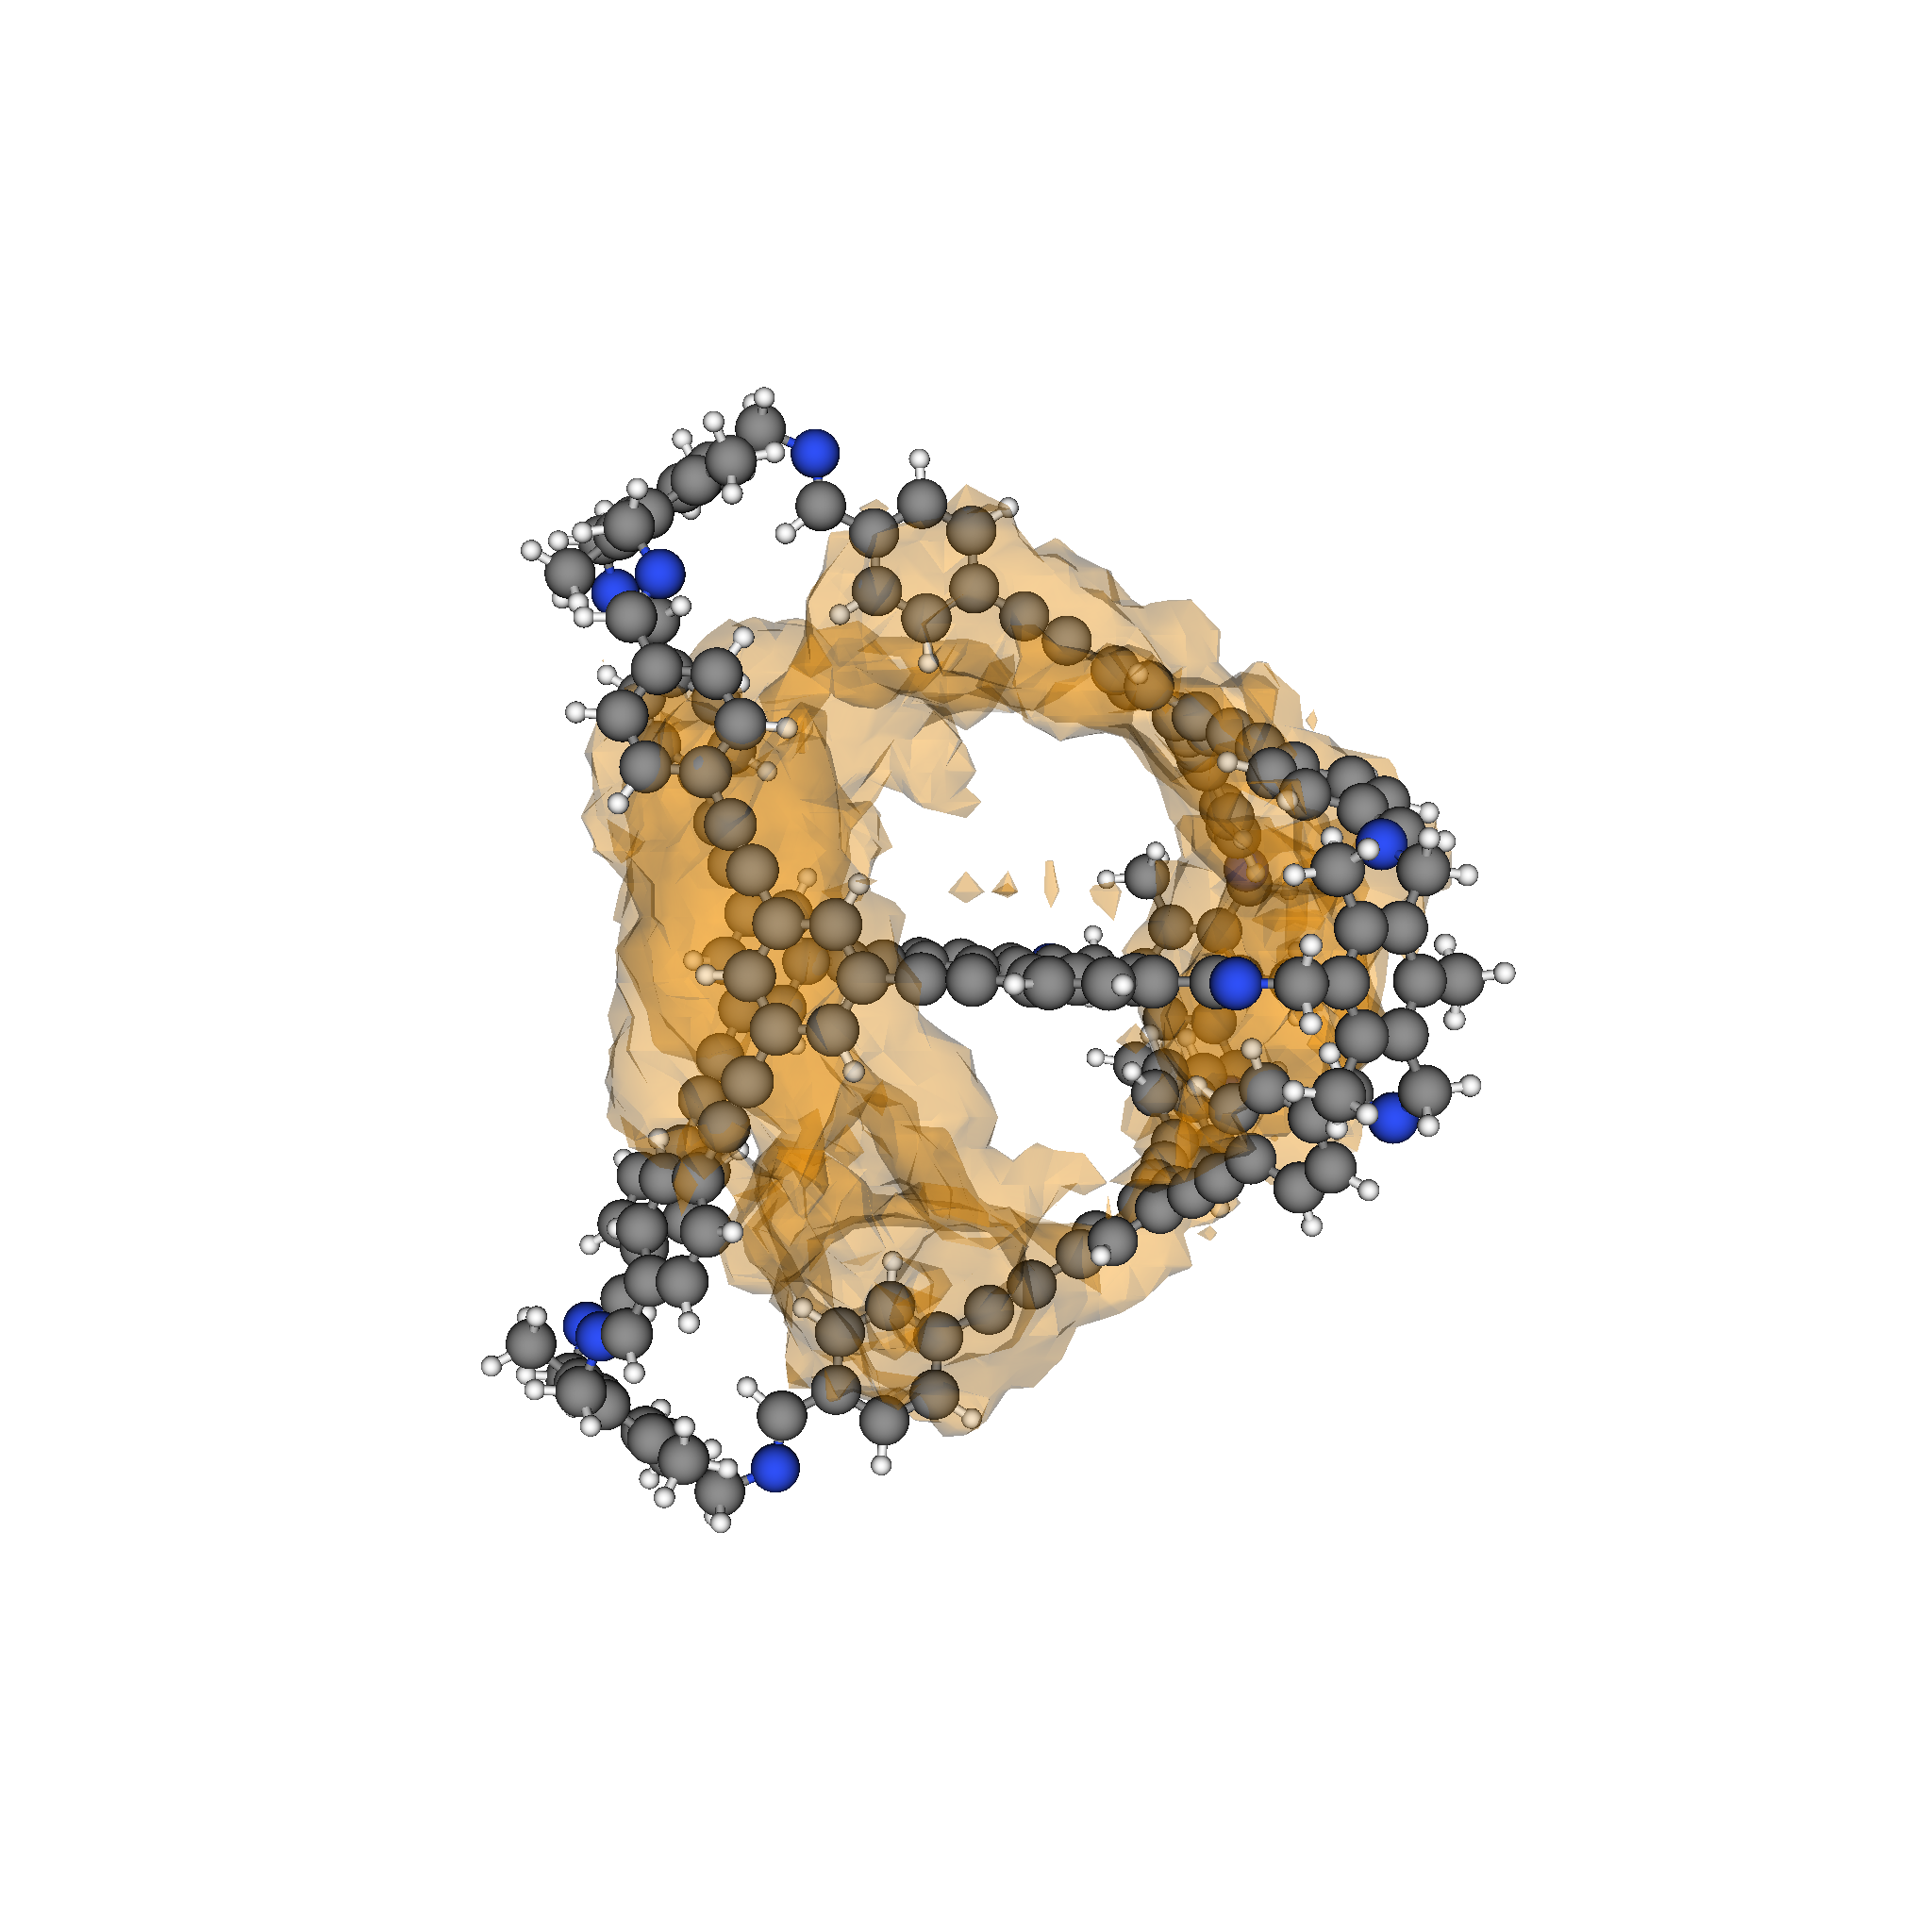
\includegraphics[width=0.275\columnwidth]{B25_nu4.png}}
	\subfloat[][$\nu=5$]{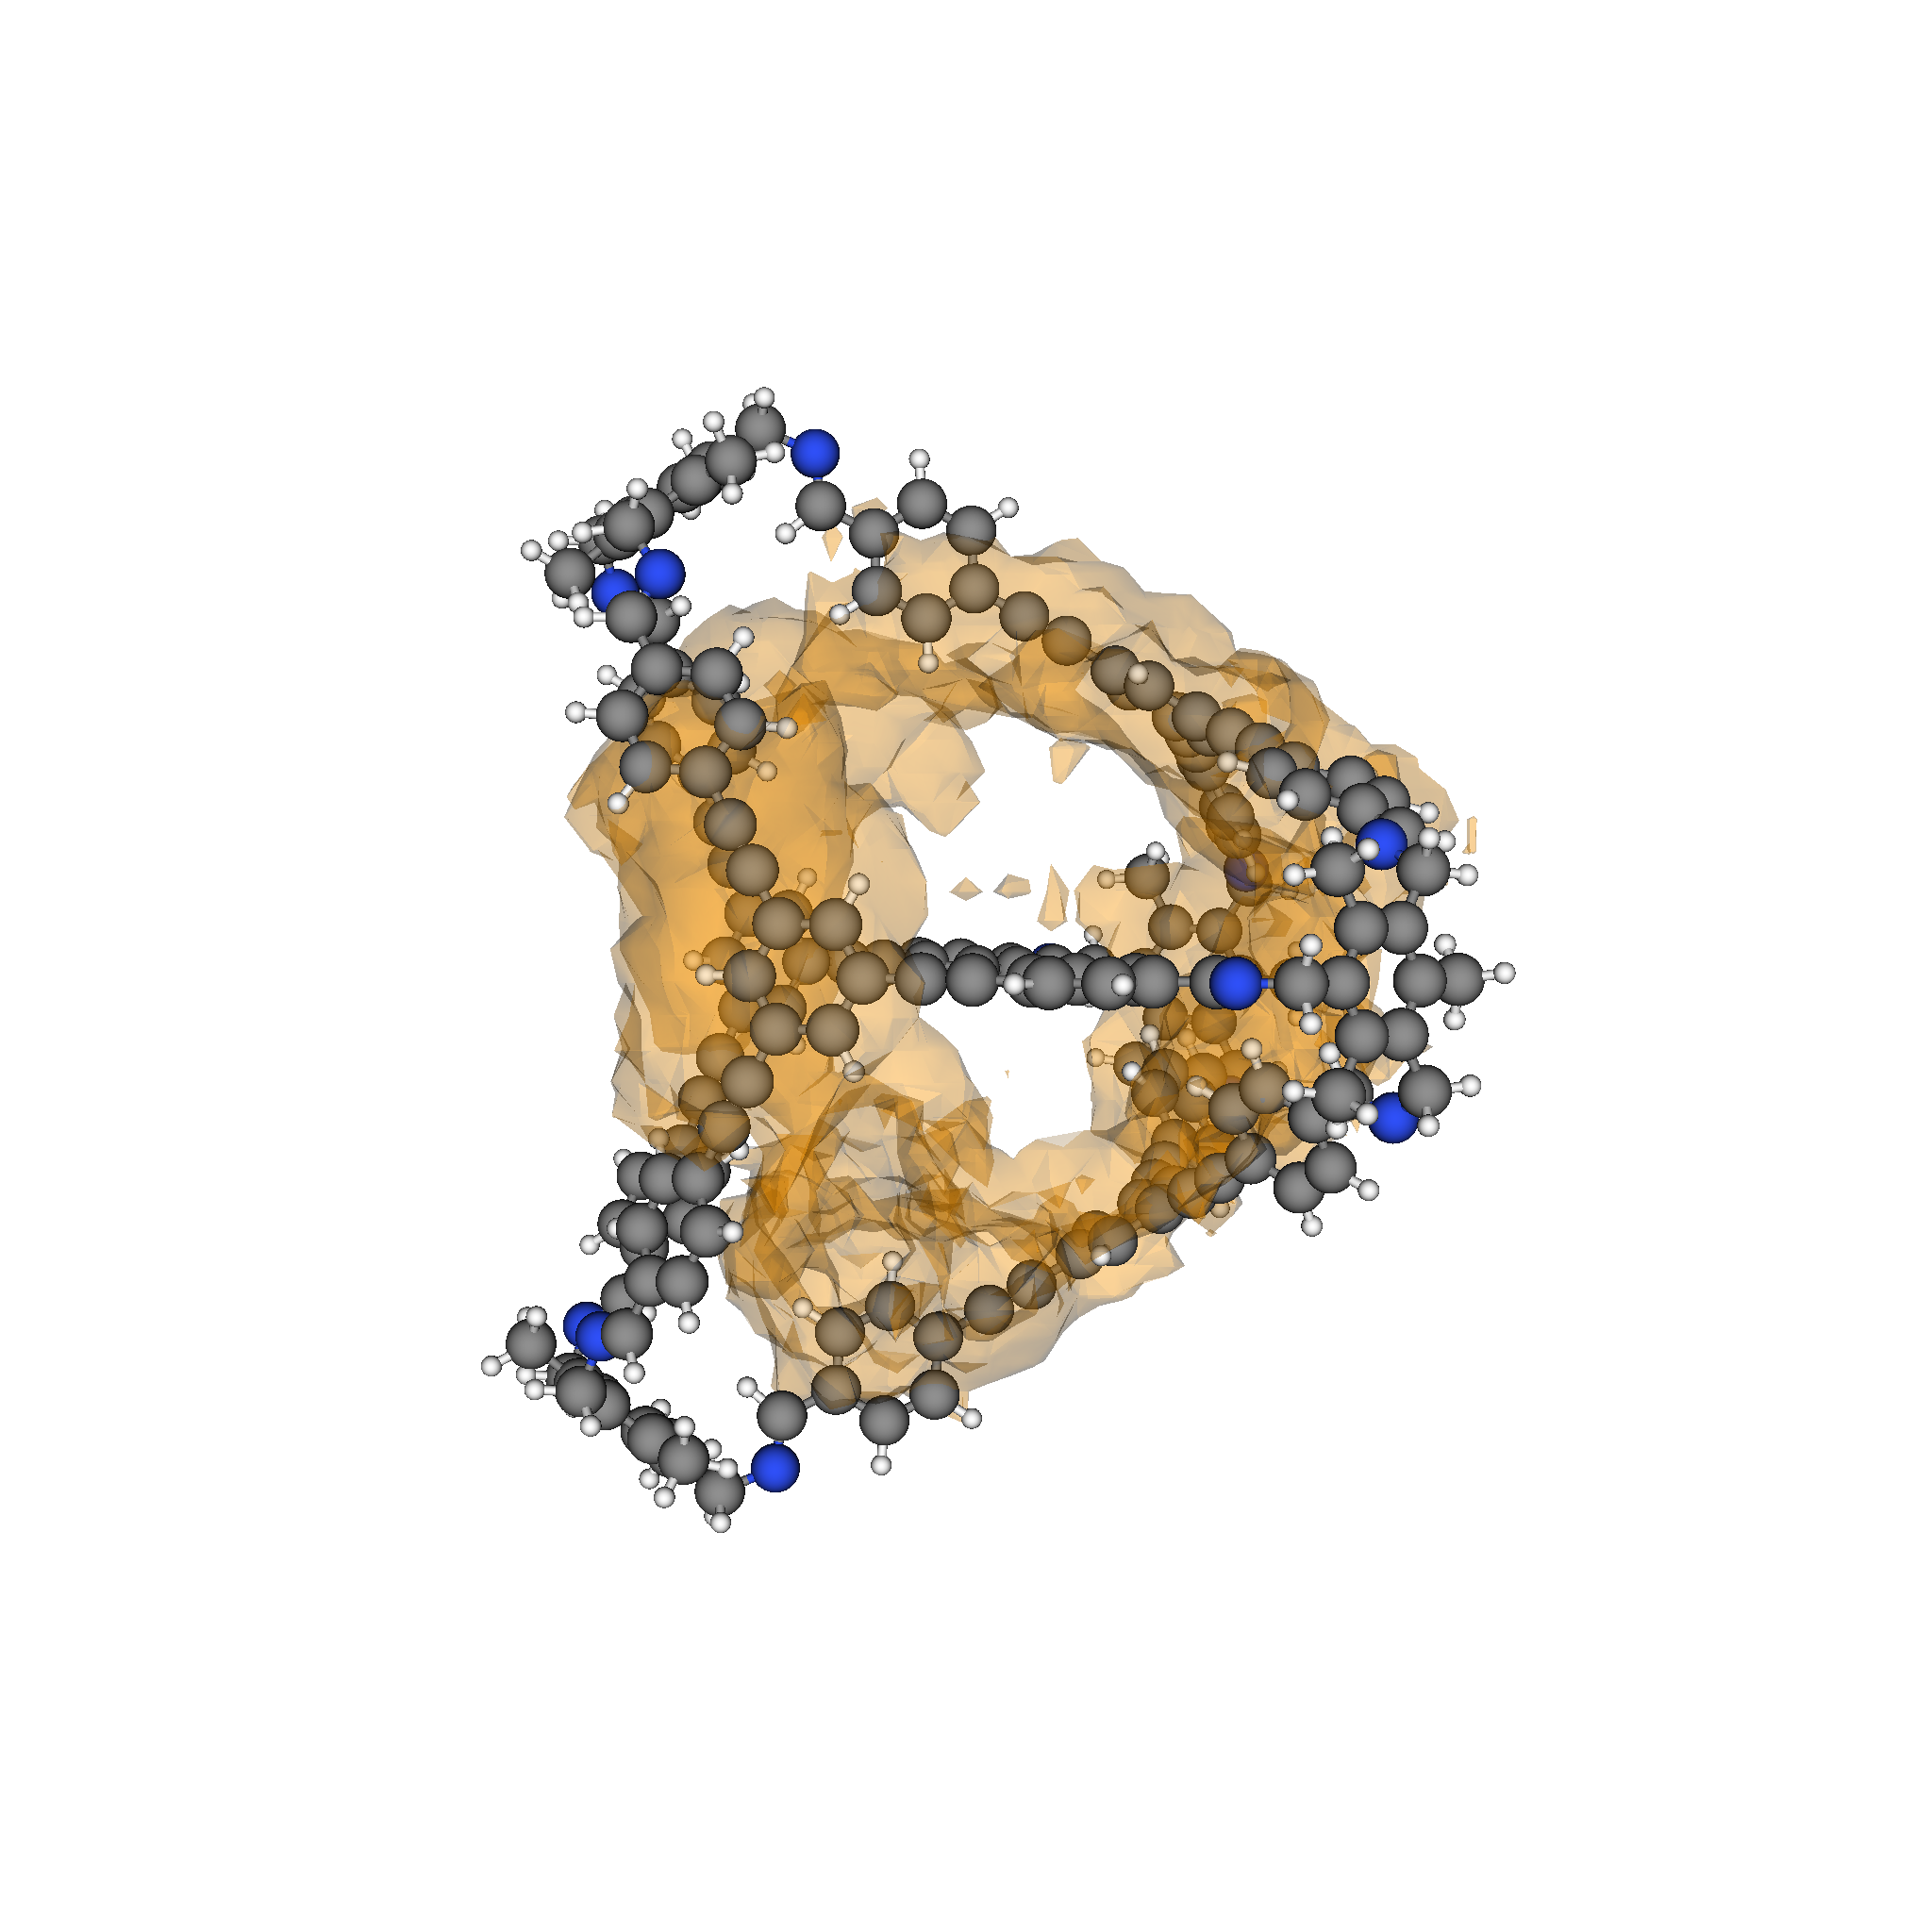
\includegraphics[width=0.275\columnwidth]{B25_nu5.png}}
	\subfloat[][$\nu=6$]{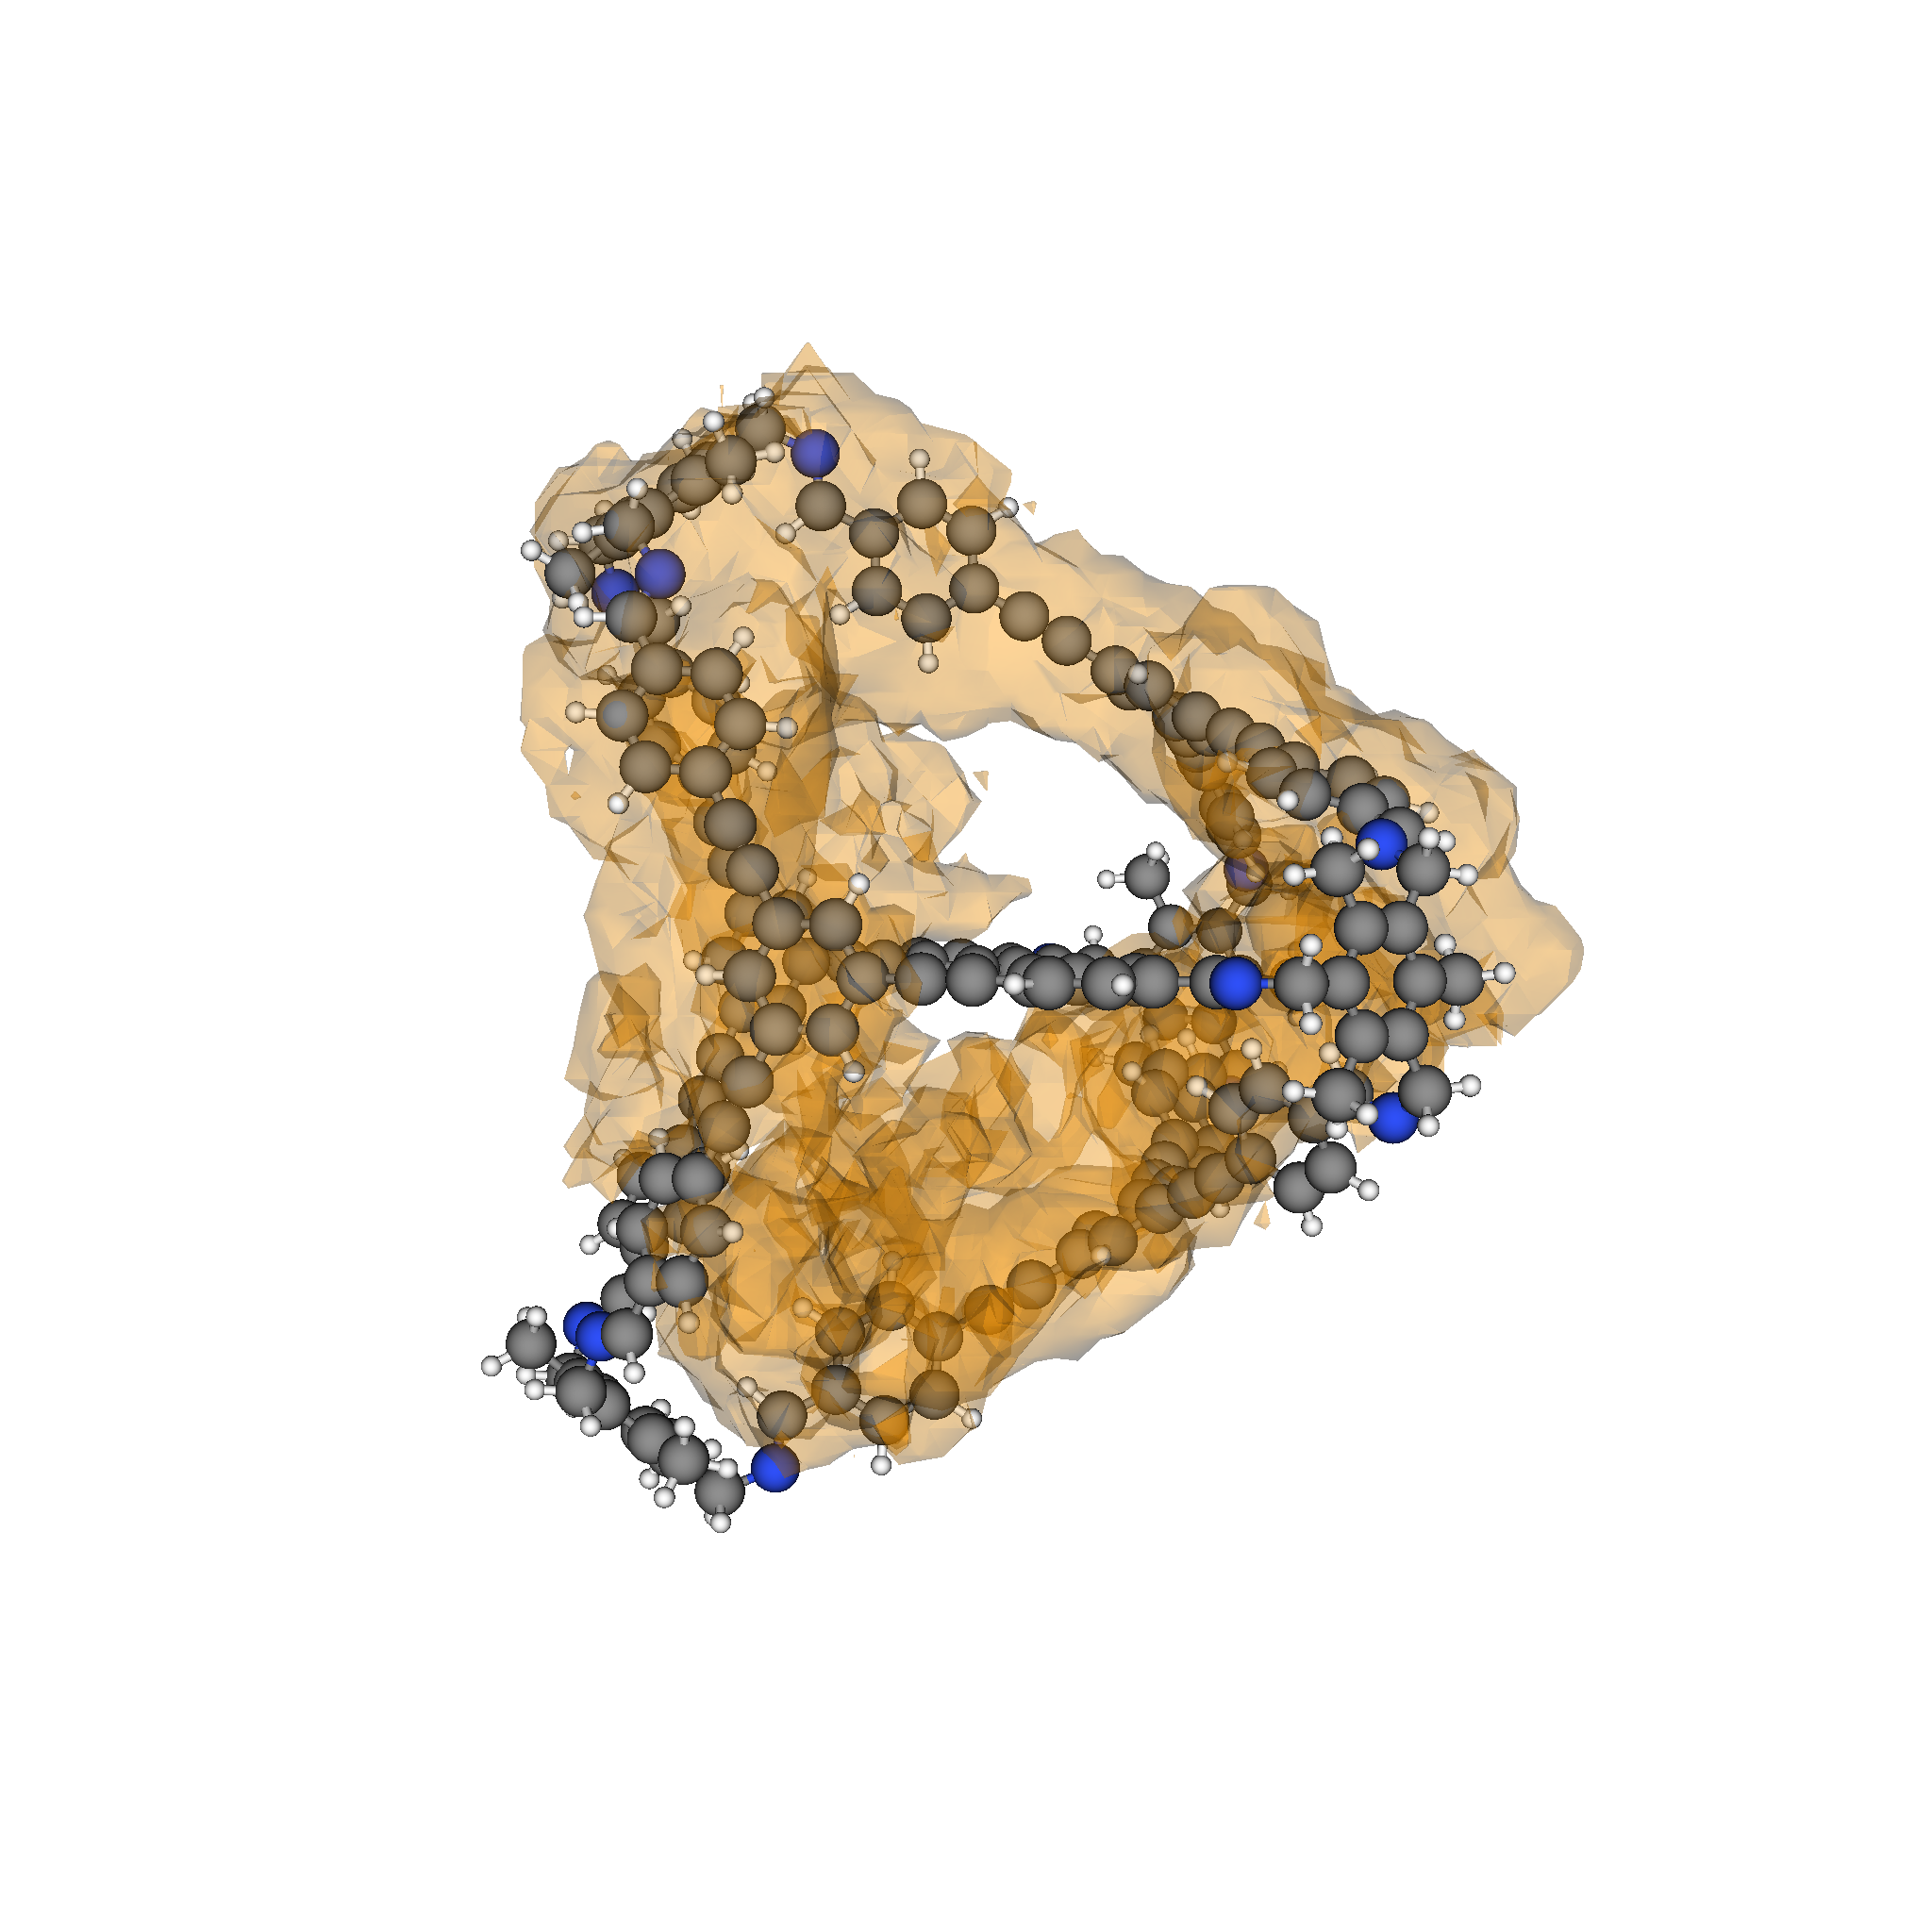
\includegraphics[width=0.275\columnwidth]{B25_nu6.png}}
	\qquad
	\subfloat[][$\nu=7$]{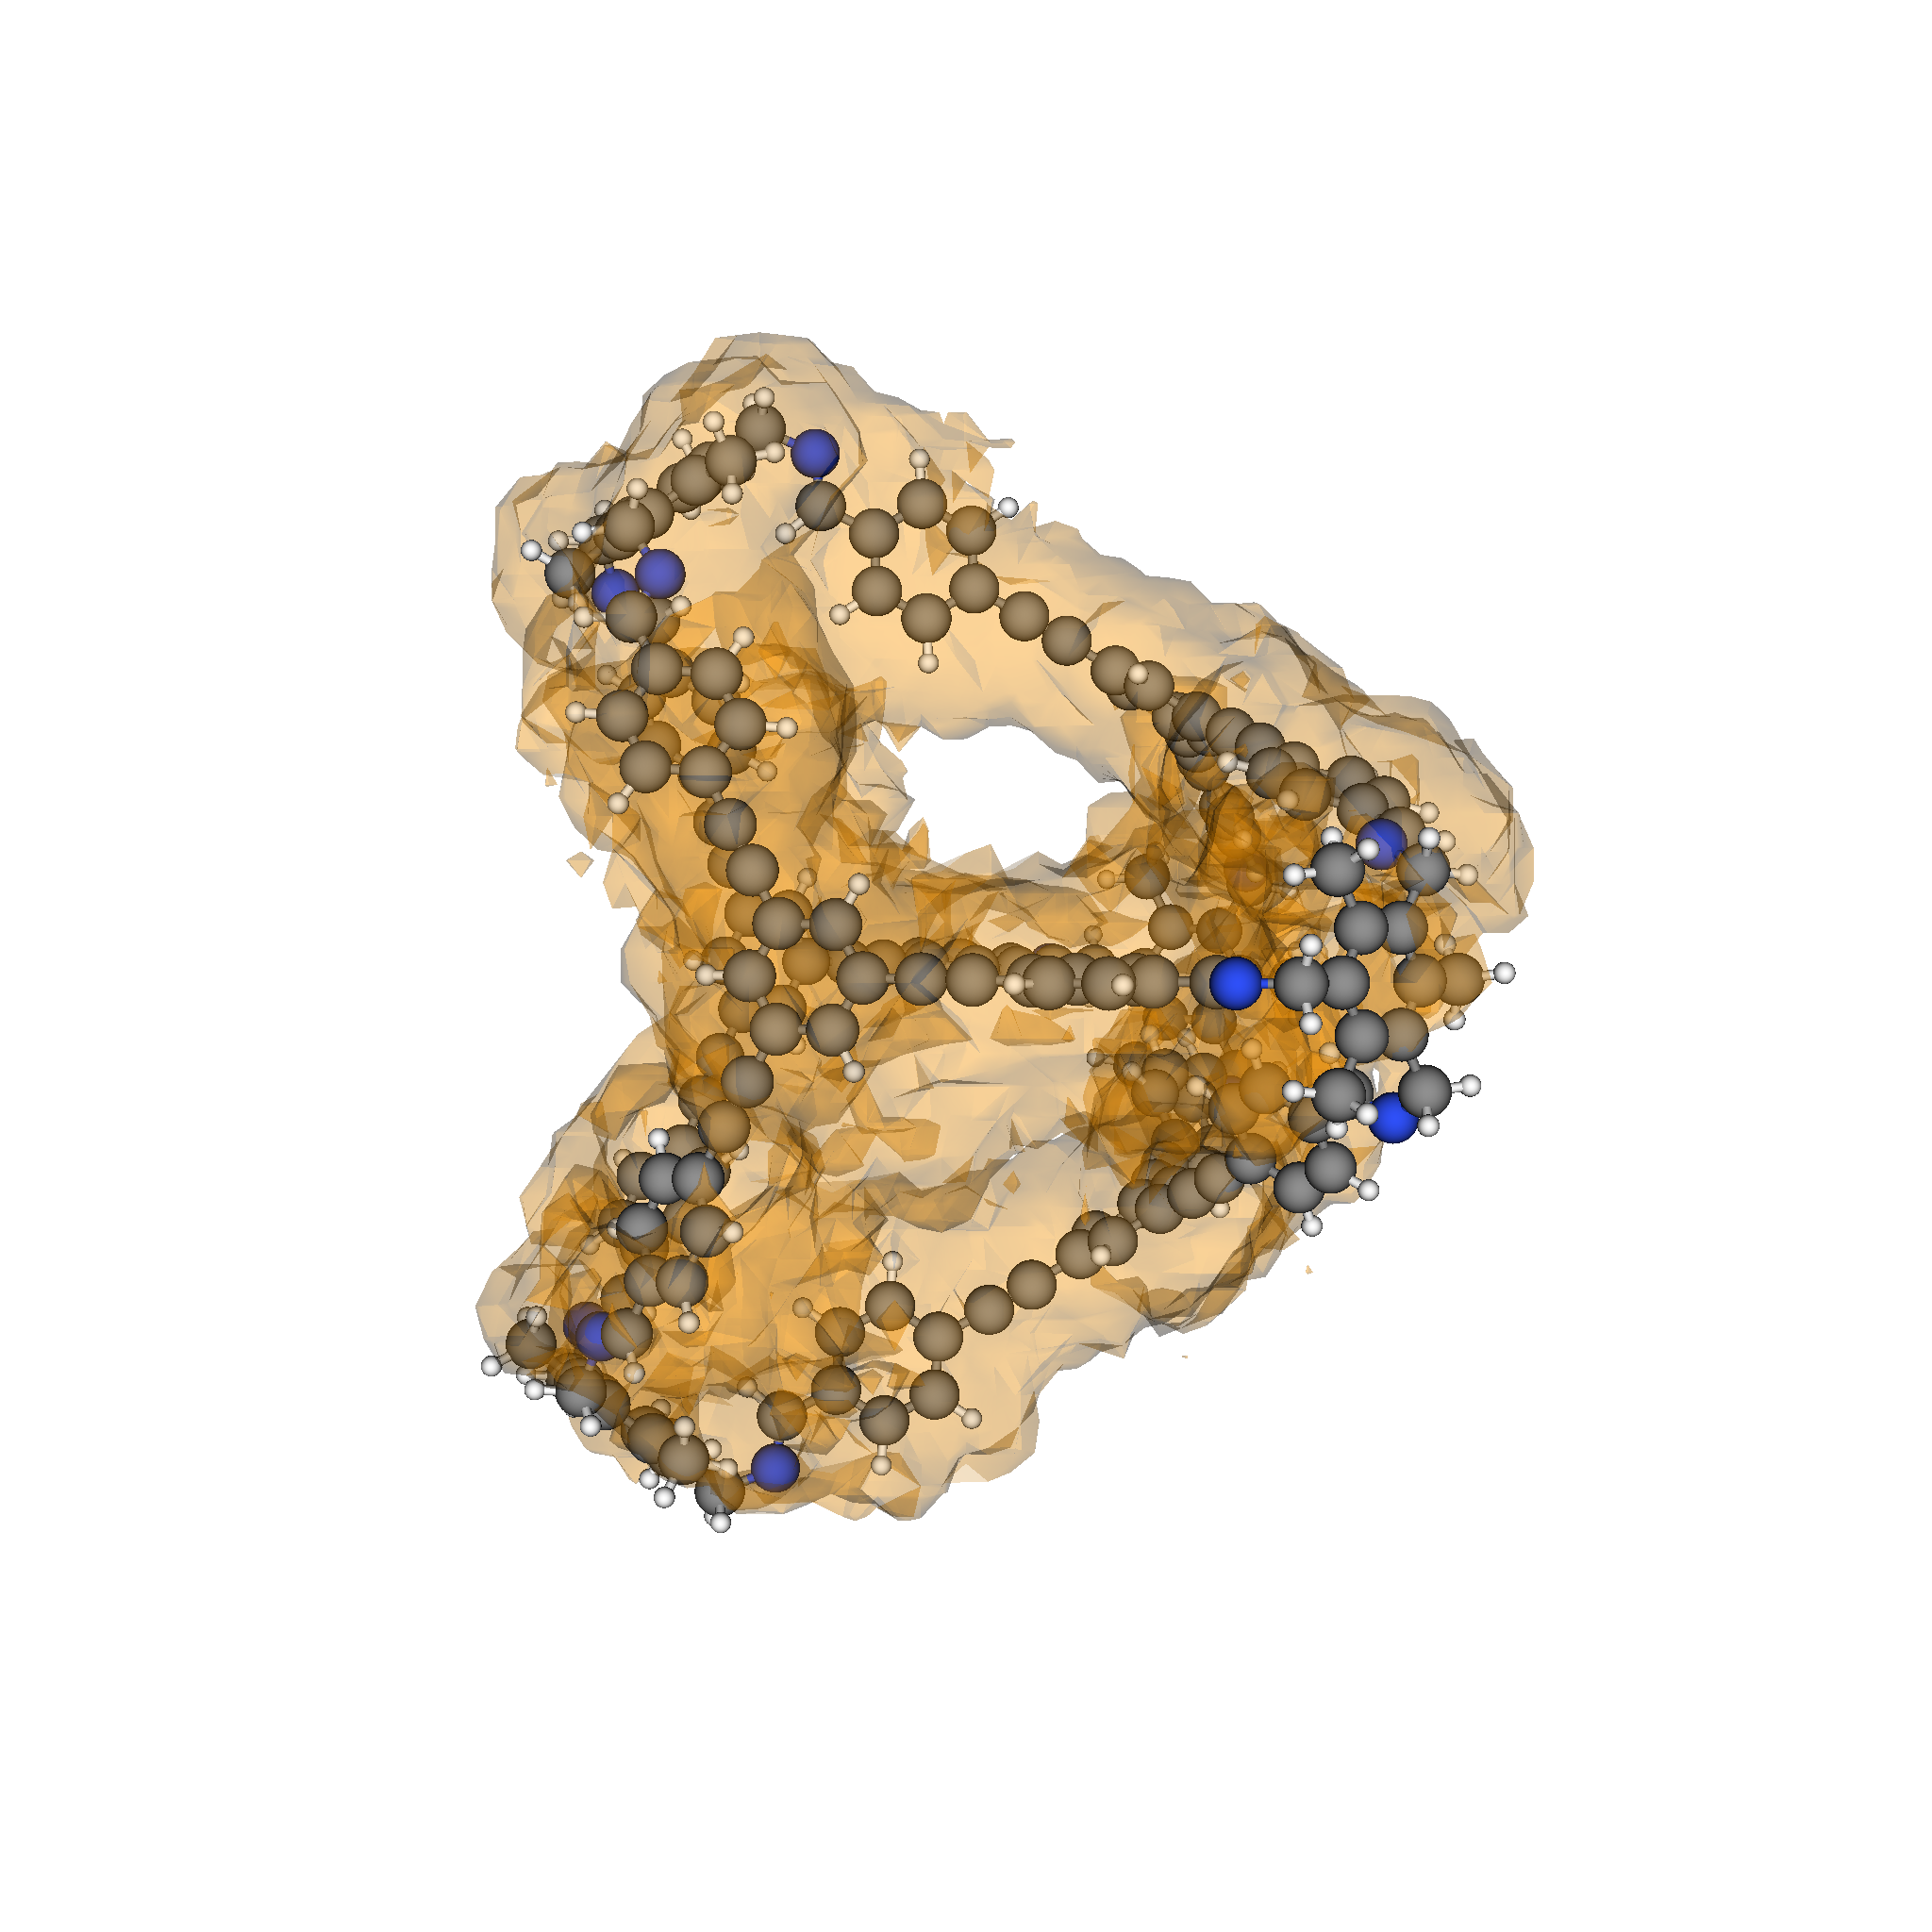
\includegraphics[width=0.275\columnwidth]{B25_nu7.png}}
	\subfloat[][$\nu=8$]{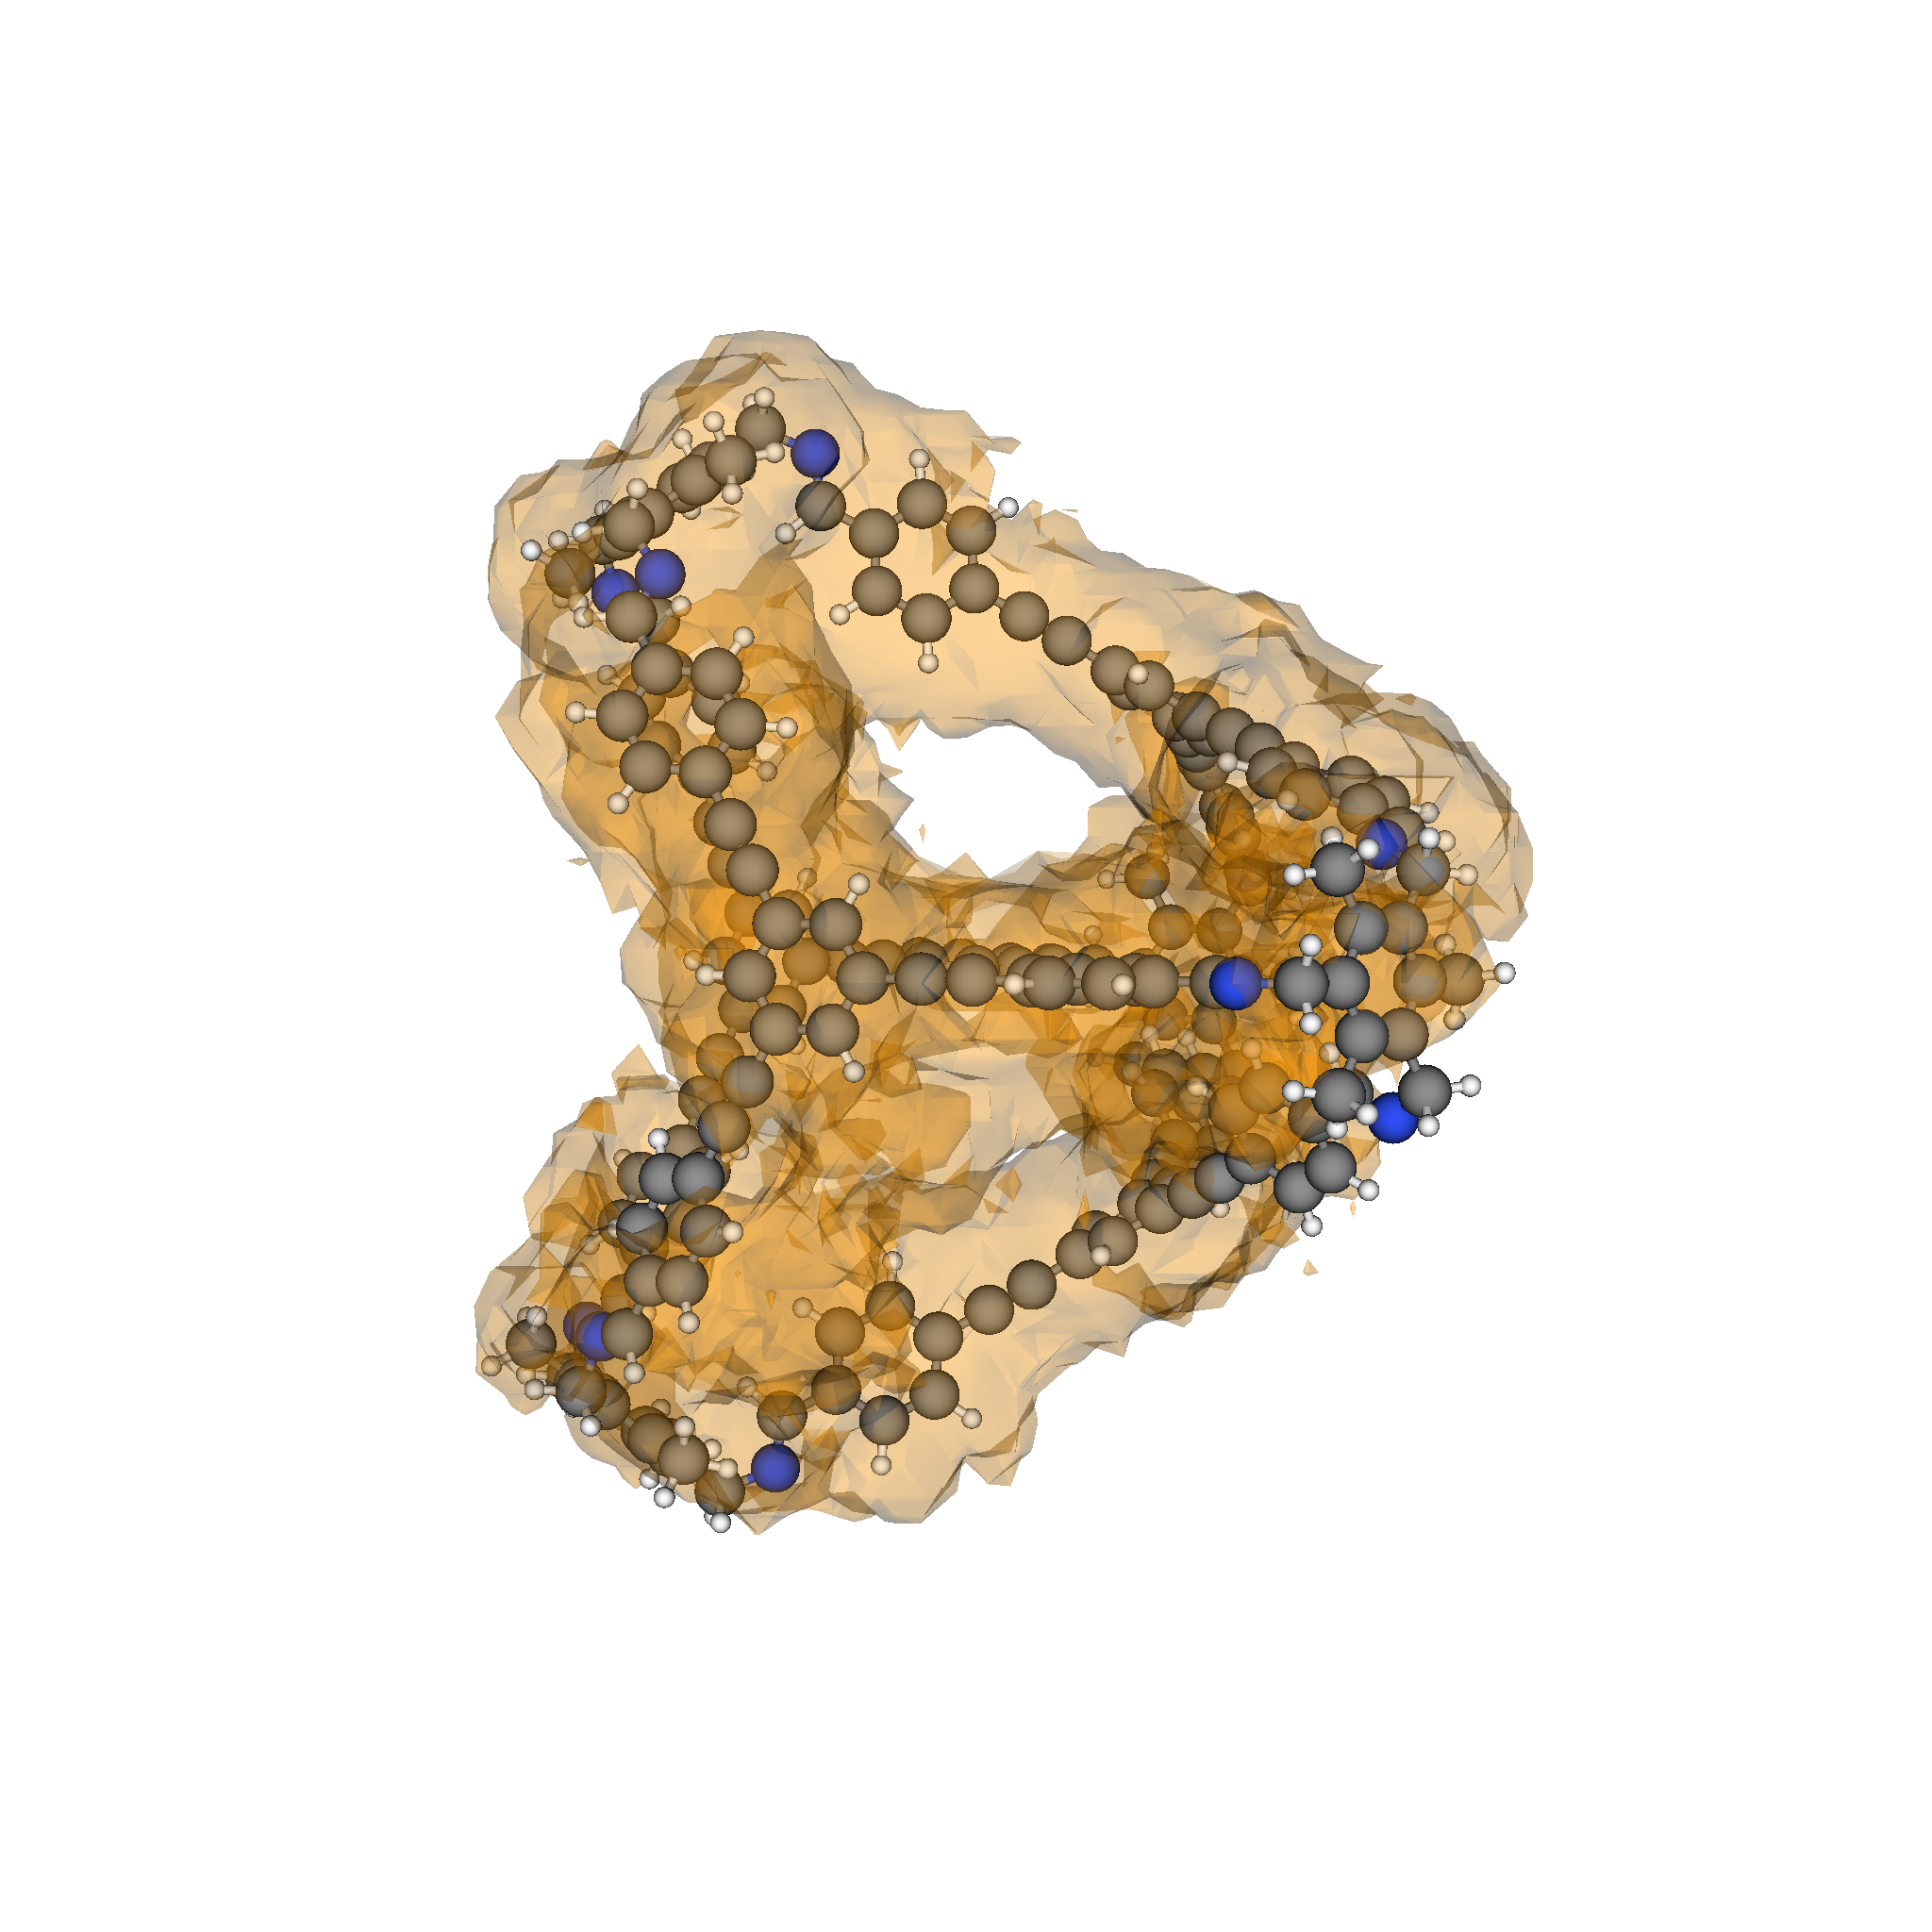
\includegraphics[width=0.275\columnwidth]{B25_nu8.png}}
	\subfloat[][$\nu=9$]{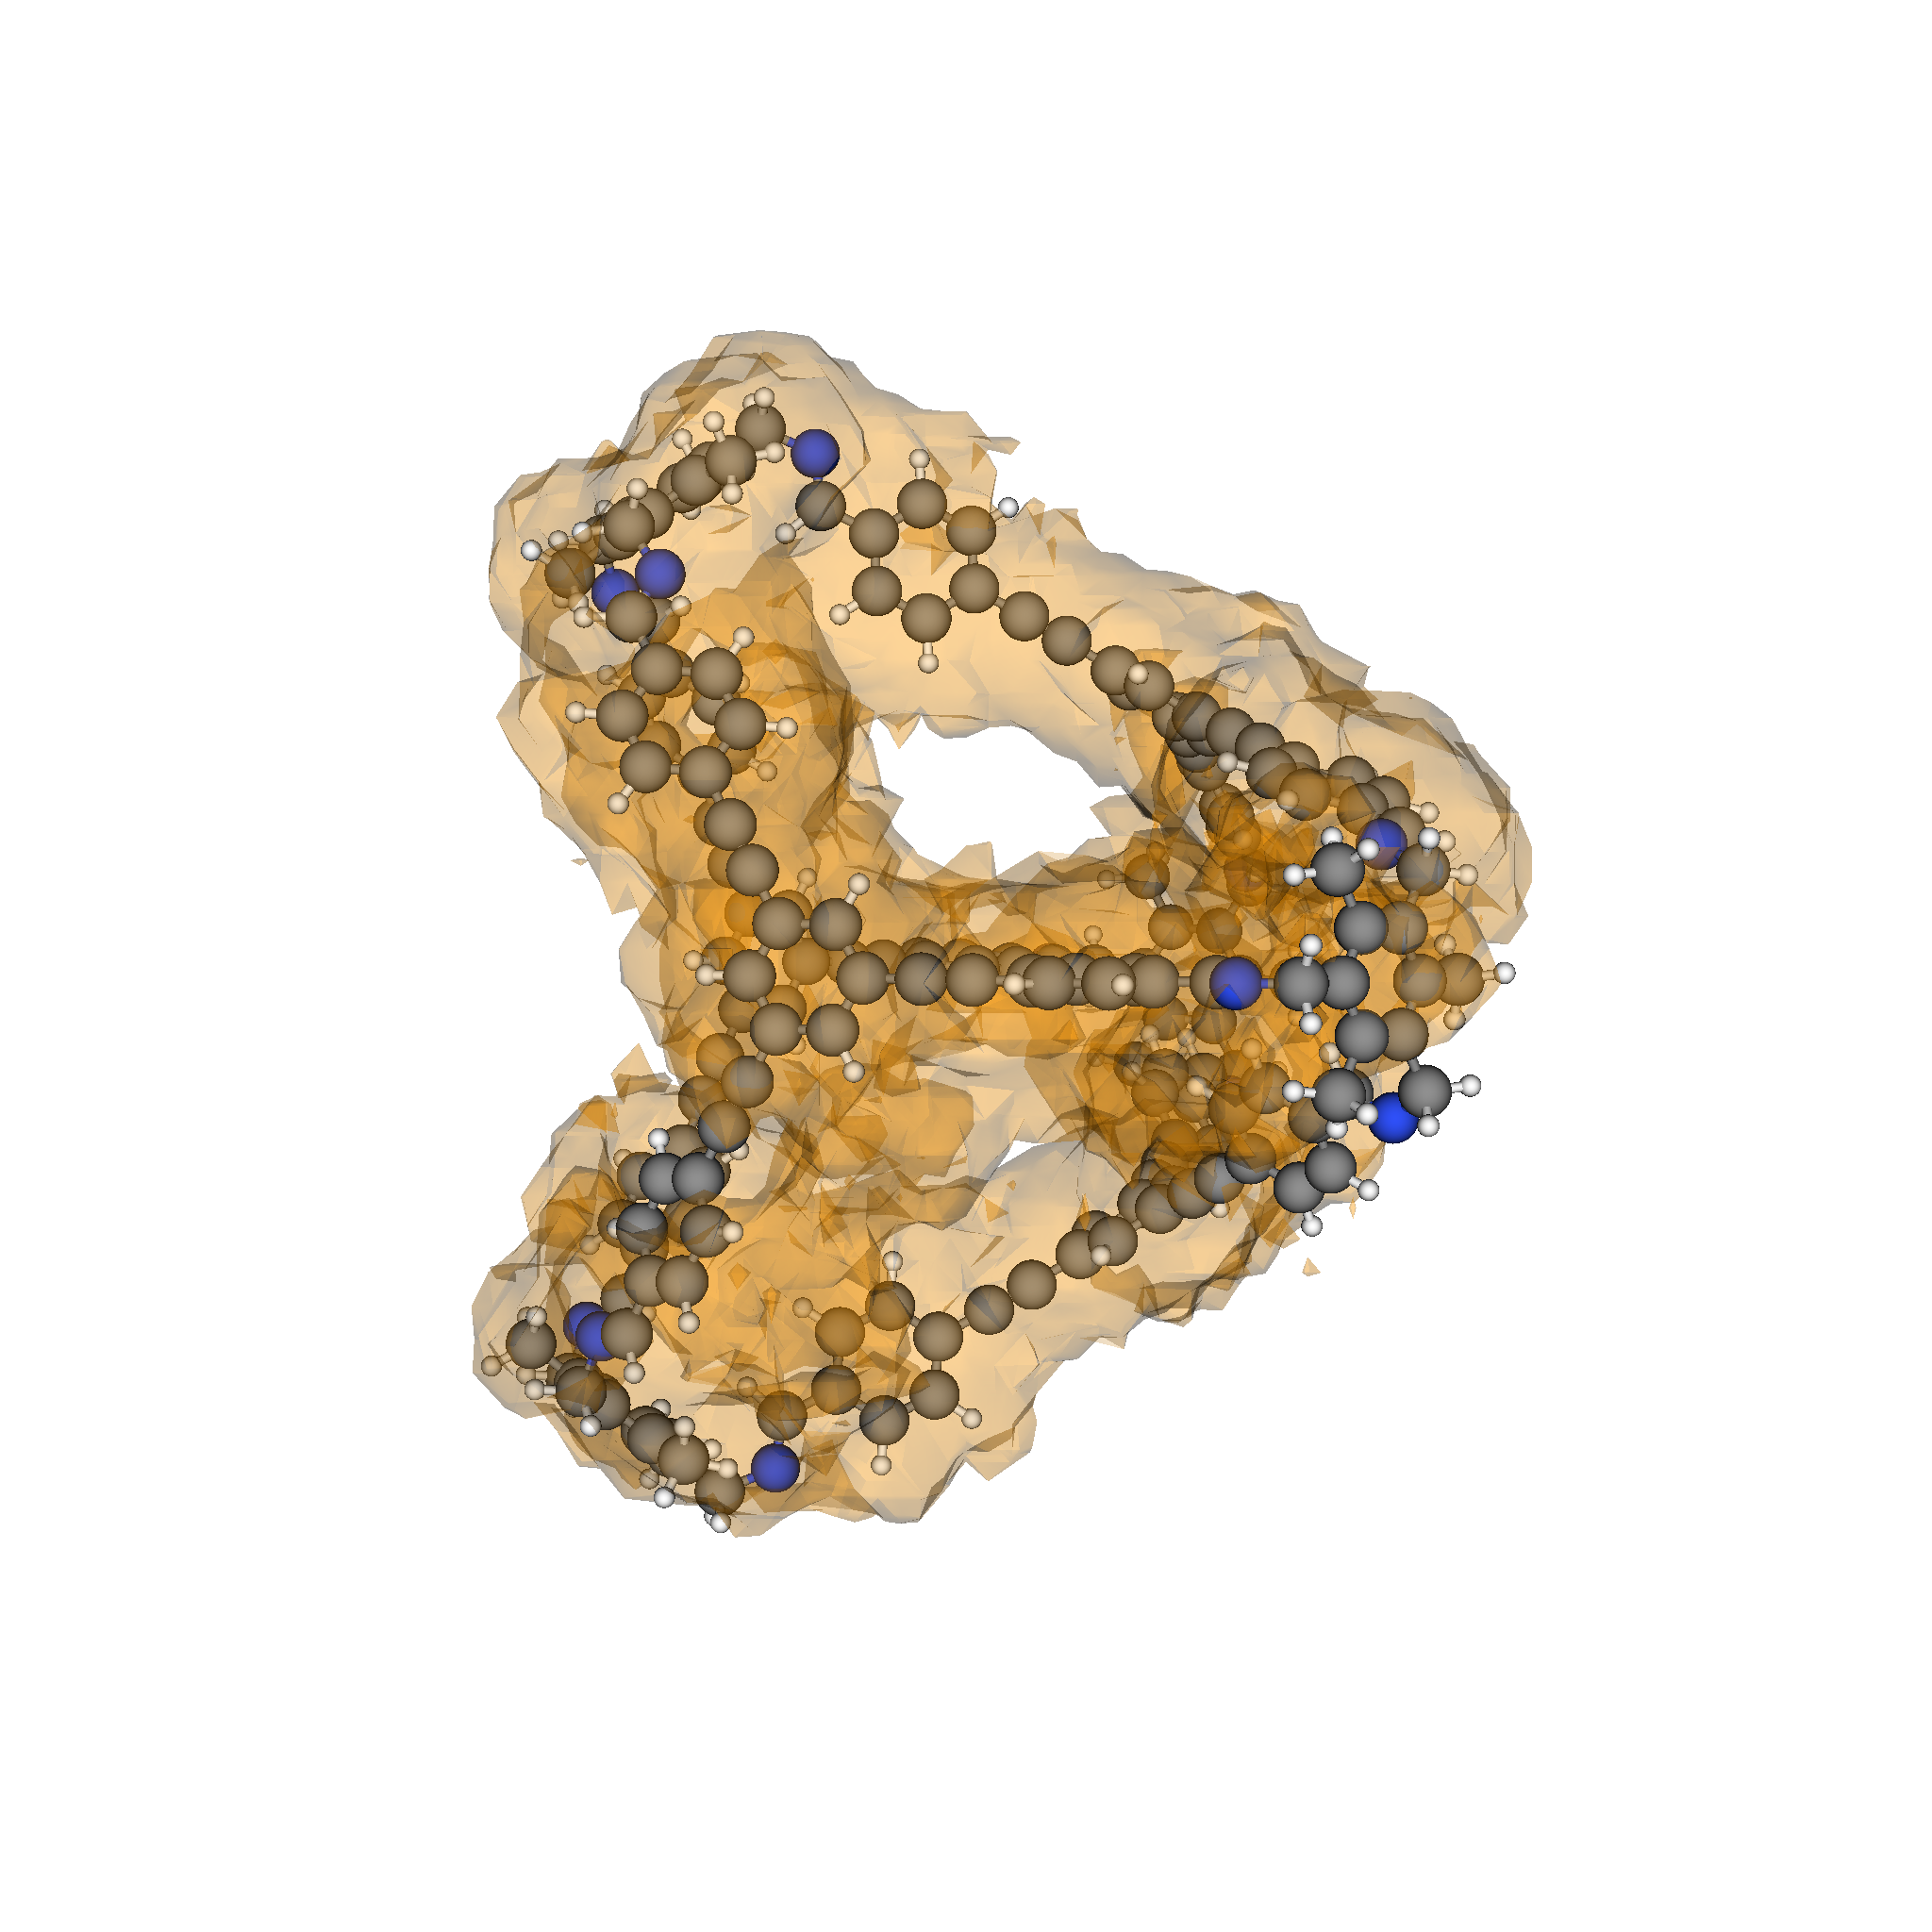
\includegraphics[width=0.275\columnwidth]{B25_nu9.png}}
	\caption{Reconstructing cage \textbf{B25} with its latent representation. (a) Exact 3D void space image of \textbf{B25}. (b-j) Reconstructions using latent representations of varying dimensions $\nu$. These are contours (0.5) of eqn.~\ref{eq:latent_space_view} with varying $\nu$. (Views from an angle to clearly see the cavity.)
	} \label{fig:cage_reconstruction}
\end{figure}

\section{\color{red} Visualizing \& interpreting the latent space of porous cages} 
The latent representations of the cavities of the porous organic cage molecules describe how each cage is composed of the eigencages and are the rows of $\mathbf{U}_\nu \mathbf{\Sigma}_\nu$ (see Fig.~\ref{fig:svd_approx}). {\color{red} Because the latent space is of too high of a dimension to visualize directly ($\nu=22$), we resort to t-Distributed Stochastic Neighbor Embedding (t-SNE) \cite{maaten2008visualizing,wattenberg2016how} to embed our learned latent space of porous cages into a two-dimensional space for visualization. 
In contrast to simply visualizing the first two dimensions of our latent space-- essentially choosing $\nu=2$ in eqn.~\ref{eq:Anu}-- t-SNE is a non-linear dimensionality reduction algorithm and hence complicated structure in the $\nu=22$-dimensional space can be retained/captured in the 2D embedding. Moreover, while  SVD prioritizes maintaining large distances in data space in the low-dimensional space, t-SNE is designed to preserve the local structure of the high-dimensional data in the low-dimensional embedding, but it also often captures global structure \cite{maaten2008visualizing}. 
A tunable parameter in t-SNE is the perplexity, a loose measure of how many neighbors each data point has \cite{maaten2008visualizing,wattenberg2016how}. We find that our clusters of cages are fairly robust to our choice of the perplexity (5, in the range recommended in Ref.~\cite{maaten2008visualizing}).
} Fig.~\ref{fig:latent_space} shows the resulting 2D embedding of the 3D porosity images of the porous cages; each cage appears as a point in this visualization of our latent cage space.

The cavities of cages within clusters in the learned latent space appear strikingly similar.
We highly encourage readers to explore our interactive visualization of the latent space at \url{simonensemble.github.io/latent-cage-space}; upon hovering the mouse over a point in latent space, an image of the cage structure displays to facilitate interpreting the latent space. Fig.~\ref{fig:latent_space} highlights a few salient clusters. The remaining clusters are shown in Fig.~\ref{fig:latent_space2}. The clustering of the cages in latent space according to the shape of their cavities is consistent with our intuition. As this clustering is learned automatically, we can easily generalize to hundreds of thousands of porous cages instead of manually grouping them together. 

\begin{figure}
\centering
	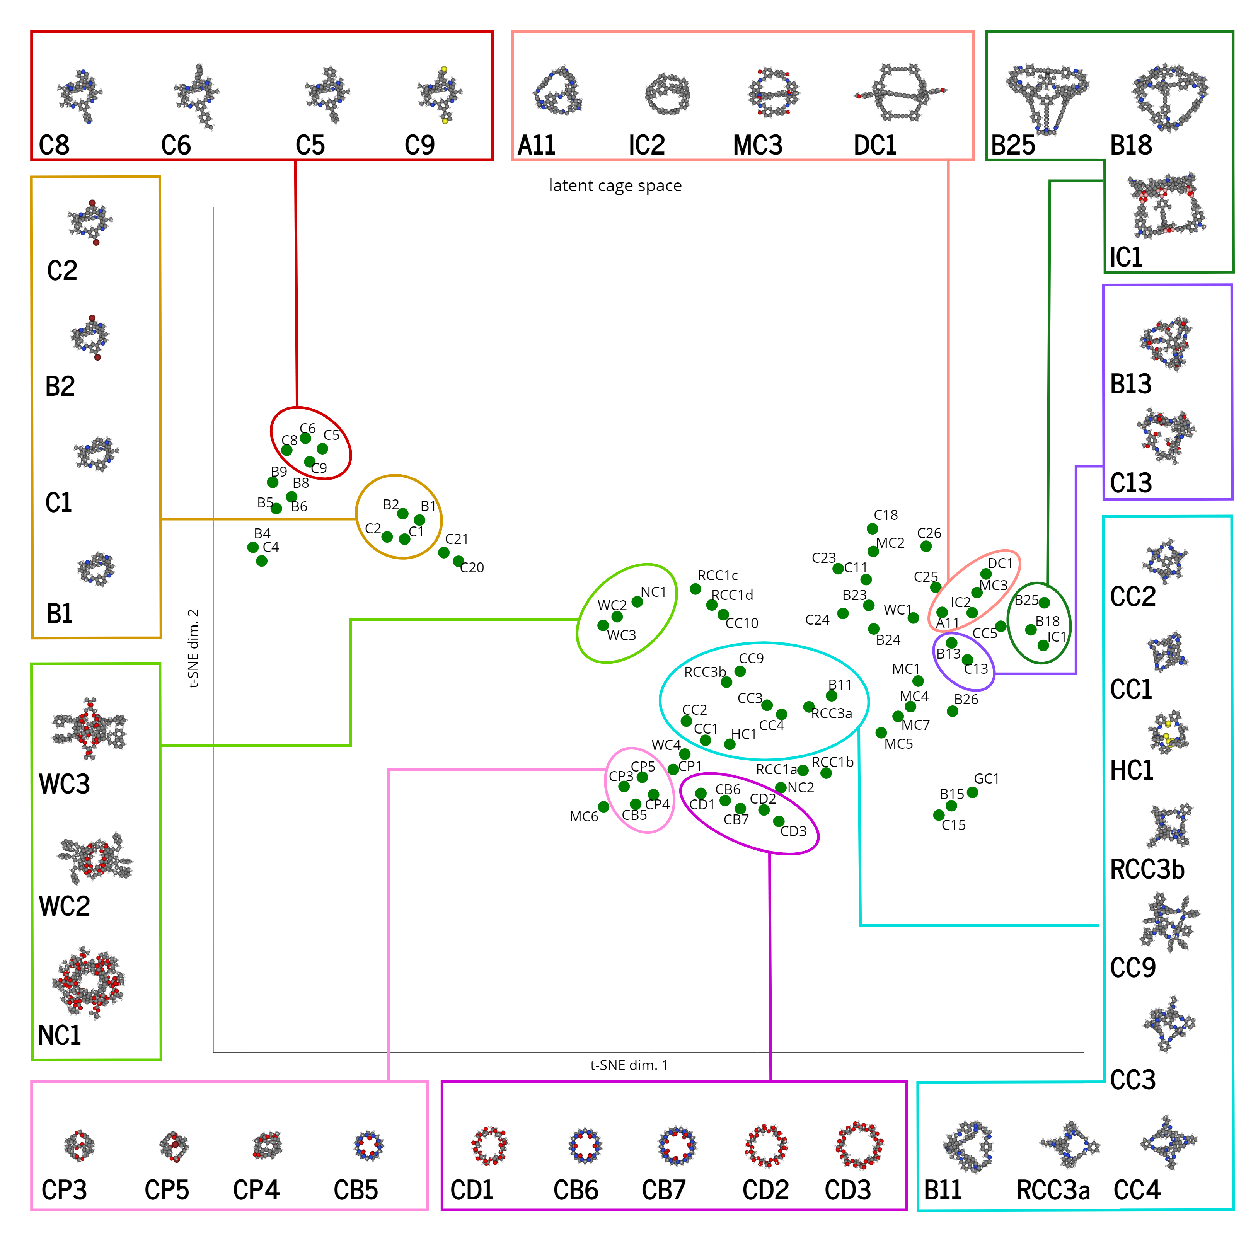
\includegraphics[width=\columnwidth]{../latent_cage_space_2D_marked_main.pdf}
	%\includegraphics[width=\columnwidth]{../latent_cage_space_2D.png}
	\caption{The latent space of cages $\mathbf{U}_\nu \mathbf{\Sigma}_\nu$ embedded into 2D by t-SNE \cite{maaten2008visualizing,wattenberg2016how}. Salient clusters are highlighted. See Fig.~\ref{fig:latent_space2} for the remaining clusters.
	} \label{fig:latent_space}
\end{figure}

We duly address that any set of invented features of a porous organic cage molecule stacked into a vector technically serves as a latent space of cages. For example, let the first entry of vector $\mathbf{x}\in \mathbb{R}^2$ be the diameter of the largest included sphere in the cavity and the second entry be the molecular mass of the cage; the set of all $\mathbf{x}$ defines a 2D latent space. However, our goal is to define a \emph{meaningful} latent space in that it is predictive of properties; i.e. neighboring materials in a good latent space will exhibit similar properties.\footnote[3]{Akin to the famous George Box adage that all models are wrong, but some are useful, we modify his adage here to ``All latent spaces are wrong, some are useful''. \cite{box1976science}} Compared to human-engineered/invented features of cages, we expect that our discovered latent space defined in $\mathbf{U}_\nu \mathbf{\Sigma}_\nu$ efficiently encodes the salient features of the cavities in porous organic cages: (i) we obtained the latent representations by optimally compressing the 3D porosity images with SVD; (ii) as Fig.~\ref{fig:cage_reconstruction} shows, the latent representation of a cage can visually reproduce the shape of its cavity; (iii) as Fig.~\ref{fig:latent_space} shows, clusters in latent space coincide with our intuition of similar cages. 

To more rigorously judge the utility of the latent space that we learned with SVD, we assess if regions of latent cage space are correlated with cage properties. First, we investigate if neighboring cages in latent space tend to exhibit similar simulated equilibrium xenon/krypton selectivities.
We place each cage molecule in an empty simulation box and compute the Henry coefficient of xenon and krypton ($T=298$ K), then subtract the Henry coefficient of helium to mimic an excess adsorption experiment, as in Patil et al. \cite{patil2016noria}. See Sec.~\ref{sec:henrydetails} for details, discussion, and comparison to experimental Xe and Kr adsorption measurements in noria (\textbf{NC2}) \cite{patil2016noria} and \textbf{CC3} \cite{chen2014separation}.
The points in Fig.~\ref{fig:latent_space_S_Xe_Kr} are colored according to the simulated Xe/Kr selectivity at infinite dilution. {\color{red} A subset of the cages, marked as `X's in Fig.~\ref{fig:latent_space_S_Xe_Kr}, possess windows that are too narrow for xenon to percolate into the cavity, according to a potential energy barrier criterion; see Sec.~\ref{sec:inaccessibility}.} Clearly, neighboring cages in the latent space are more likely to exhibit similar Xe/Kr selectivities than cages further apart. Despite atom type not being explicitly fed into SVD to learn the latent cage space, the information about the shape of the cavity encoded into the latent representation is predictive of the simulated Xe/Kr selectivity {\color{red} in the isolated cage molecule. As a word of caution, however, we explain in the Discussion that the simulated Xe/Kr selectivity of an isolated cage is not necessarily a quality prediction of the simulated Xe/Kr selectivity in the porous cage solid where the cage molecules are packed together.}
Second, we investigate if the molecule and cavity diameter of the cages computed by \texttt{pywindow} \cite{miklitz2018pywindow} are correlated with the location of a cage in latent space. Fig.~\ref{fig:cage_space_colored_by_diams_2D} clearly shows that cages nearby in latent space have a strong tendency to possess similar molecule and cavity diameters. Note that \textbf{MC6}, the largest cage in the database, appears to be an outlier. 
Finally, Fig.~\ref{fig:cage_space_colored_by_nb_windows} shows that our latent representations nicely cluster together cages with the same number of windows in which gas molecules can enter the cavity.
Together, Figs.~\ref{fig:latent_space_S_Xe_Kr}, \ref{fig:cage_space_colored_by_diams_2D}, and \ref{fig:cage_space_colored_by_nb_windows} show that our latent representation of porous cage molecules is useful for predicting properties that are correlated with the shape of the cavity (as is the case for Xe/Kr selectivity \cite{sikora2012thermodynamic,simon2015best}) and thus lends a meaningful notion of similarity between two cage molecules.

\begin{figure}
\centering
	\includegraphics[width=\columnwidth]{../cage_space_colored_by_S_Xe_Kr.pdf}
	\caption{The latent space of cages $\mathbf{U}_\nu \mathbf{\Sigma}_\nu$ embedded into 2D by t-SNE \cite{maaten2008visualizing,wattenberg2016how}. The color of points represents the simulated Xe/Kr selectivity of an isolated cage molecule in an empty box at 298 K. Points nearby in the latent cage space are likely to exhibit similar Xe/Kr selectivities. Cages marked with `X' have windows too narrow for xenon to percolate into the cavity.
	} \label{fig:latent_space_S_Xe_Kr}
\end{figure}

\subsection{A walk through latent cage space}
\label{sec:latentwalk}
G\'{o}mez-Bombarelli et al. \cite{gomez2018automatic} encoded SMILES strings of molecules into a latent space using neural networks and generated novel molecules by walking through latent molecule space. van Deursen and Reymond coin this as ``chemical space travel'' \cite{van2007chemical}. Similarly, we show in Fig~\ref{fig:walk_in_latent_space} that we can interpolate between two given cages in the $\nu=22$ dimensional latent cage space to see how one cage morphs into another.
While an interesting exercise to help interpret the latent space, walking in our latent cage space may be of limited utility since it remains unclear of how to synthesize a cage with a given cavity shape.


\begin{figure}
\centering
	\subfloat[][\textbf{NC2}]{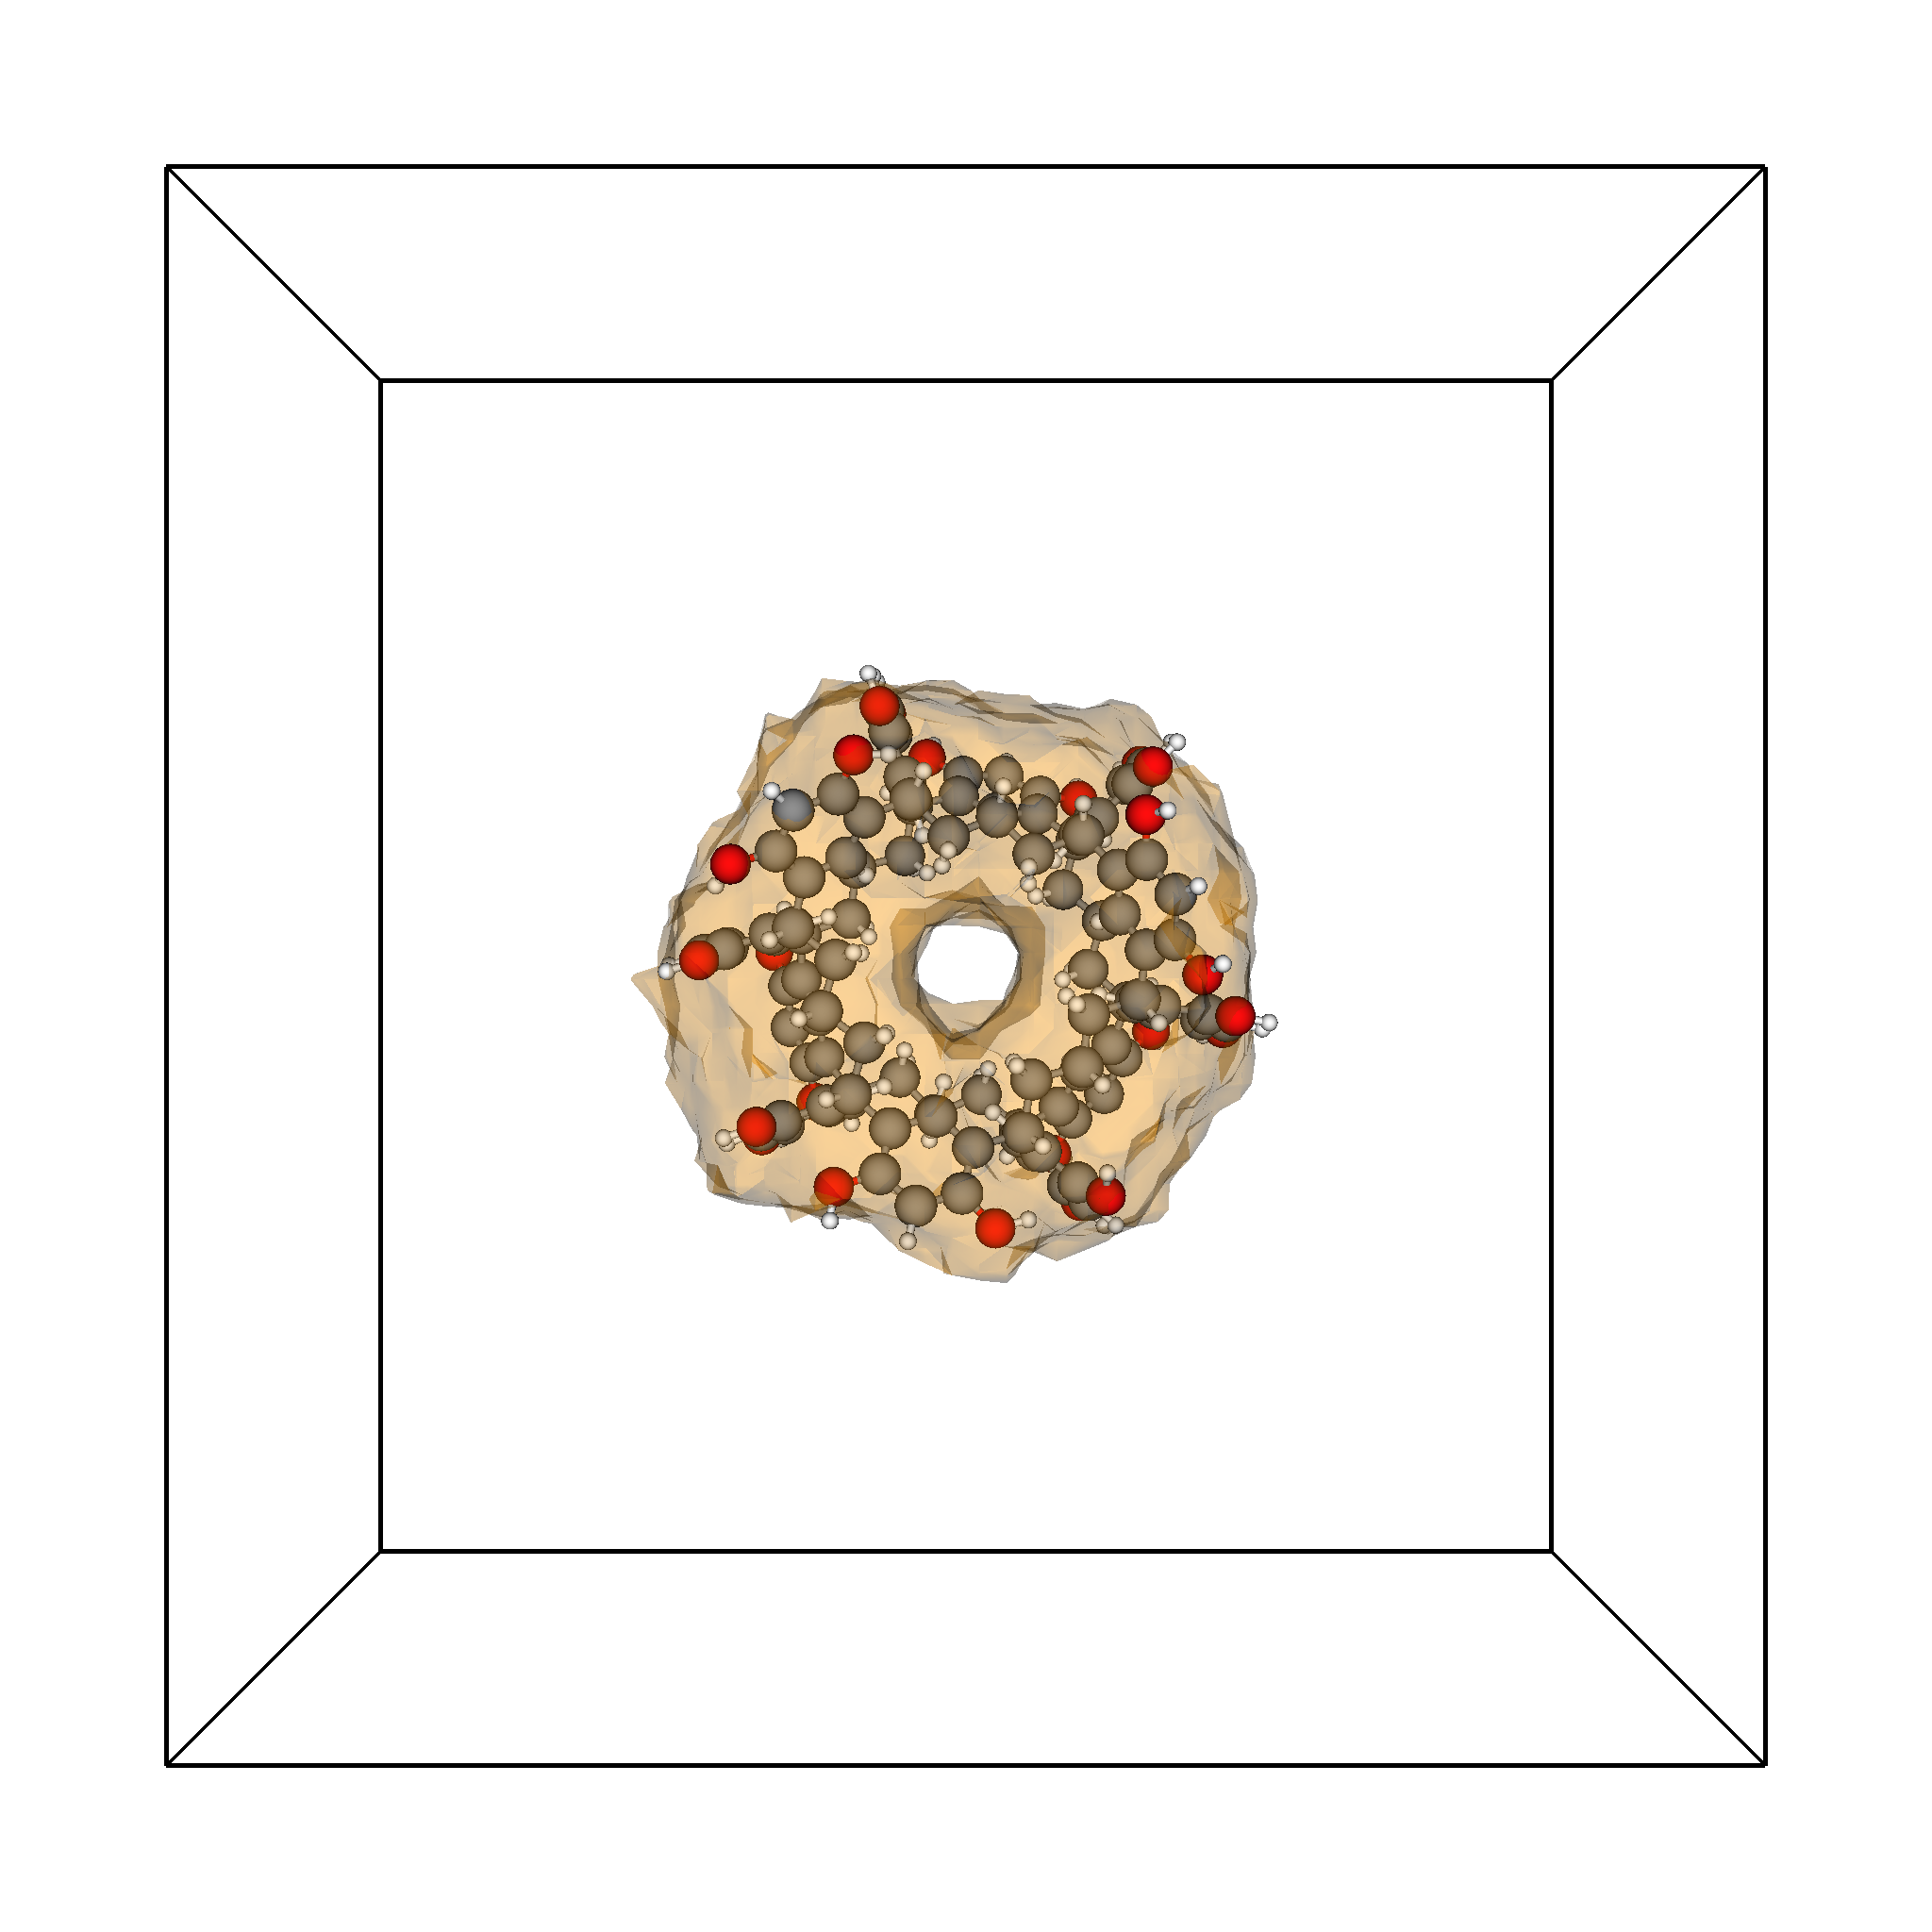
\includegraphics[width=0.165\columnwidth]{NC2_latent.png}}
	\subfloat[][]{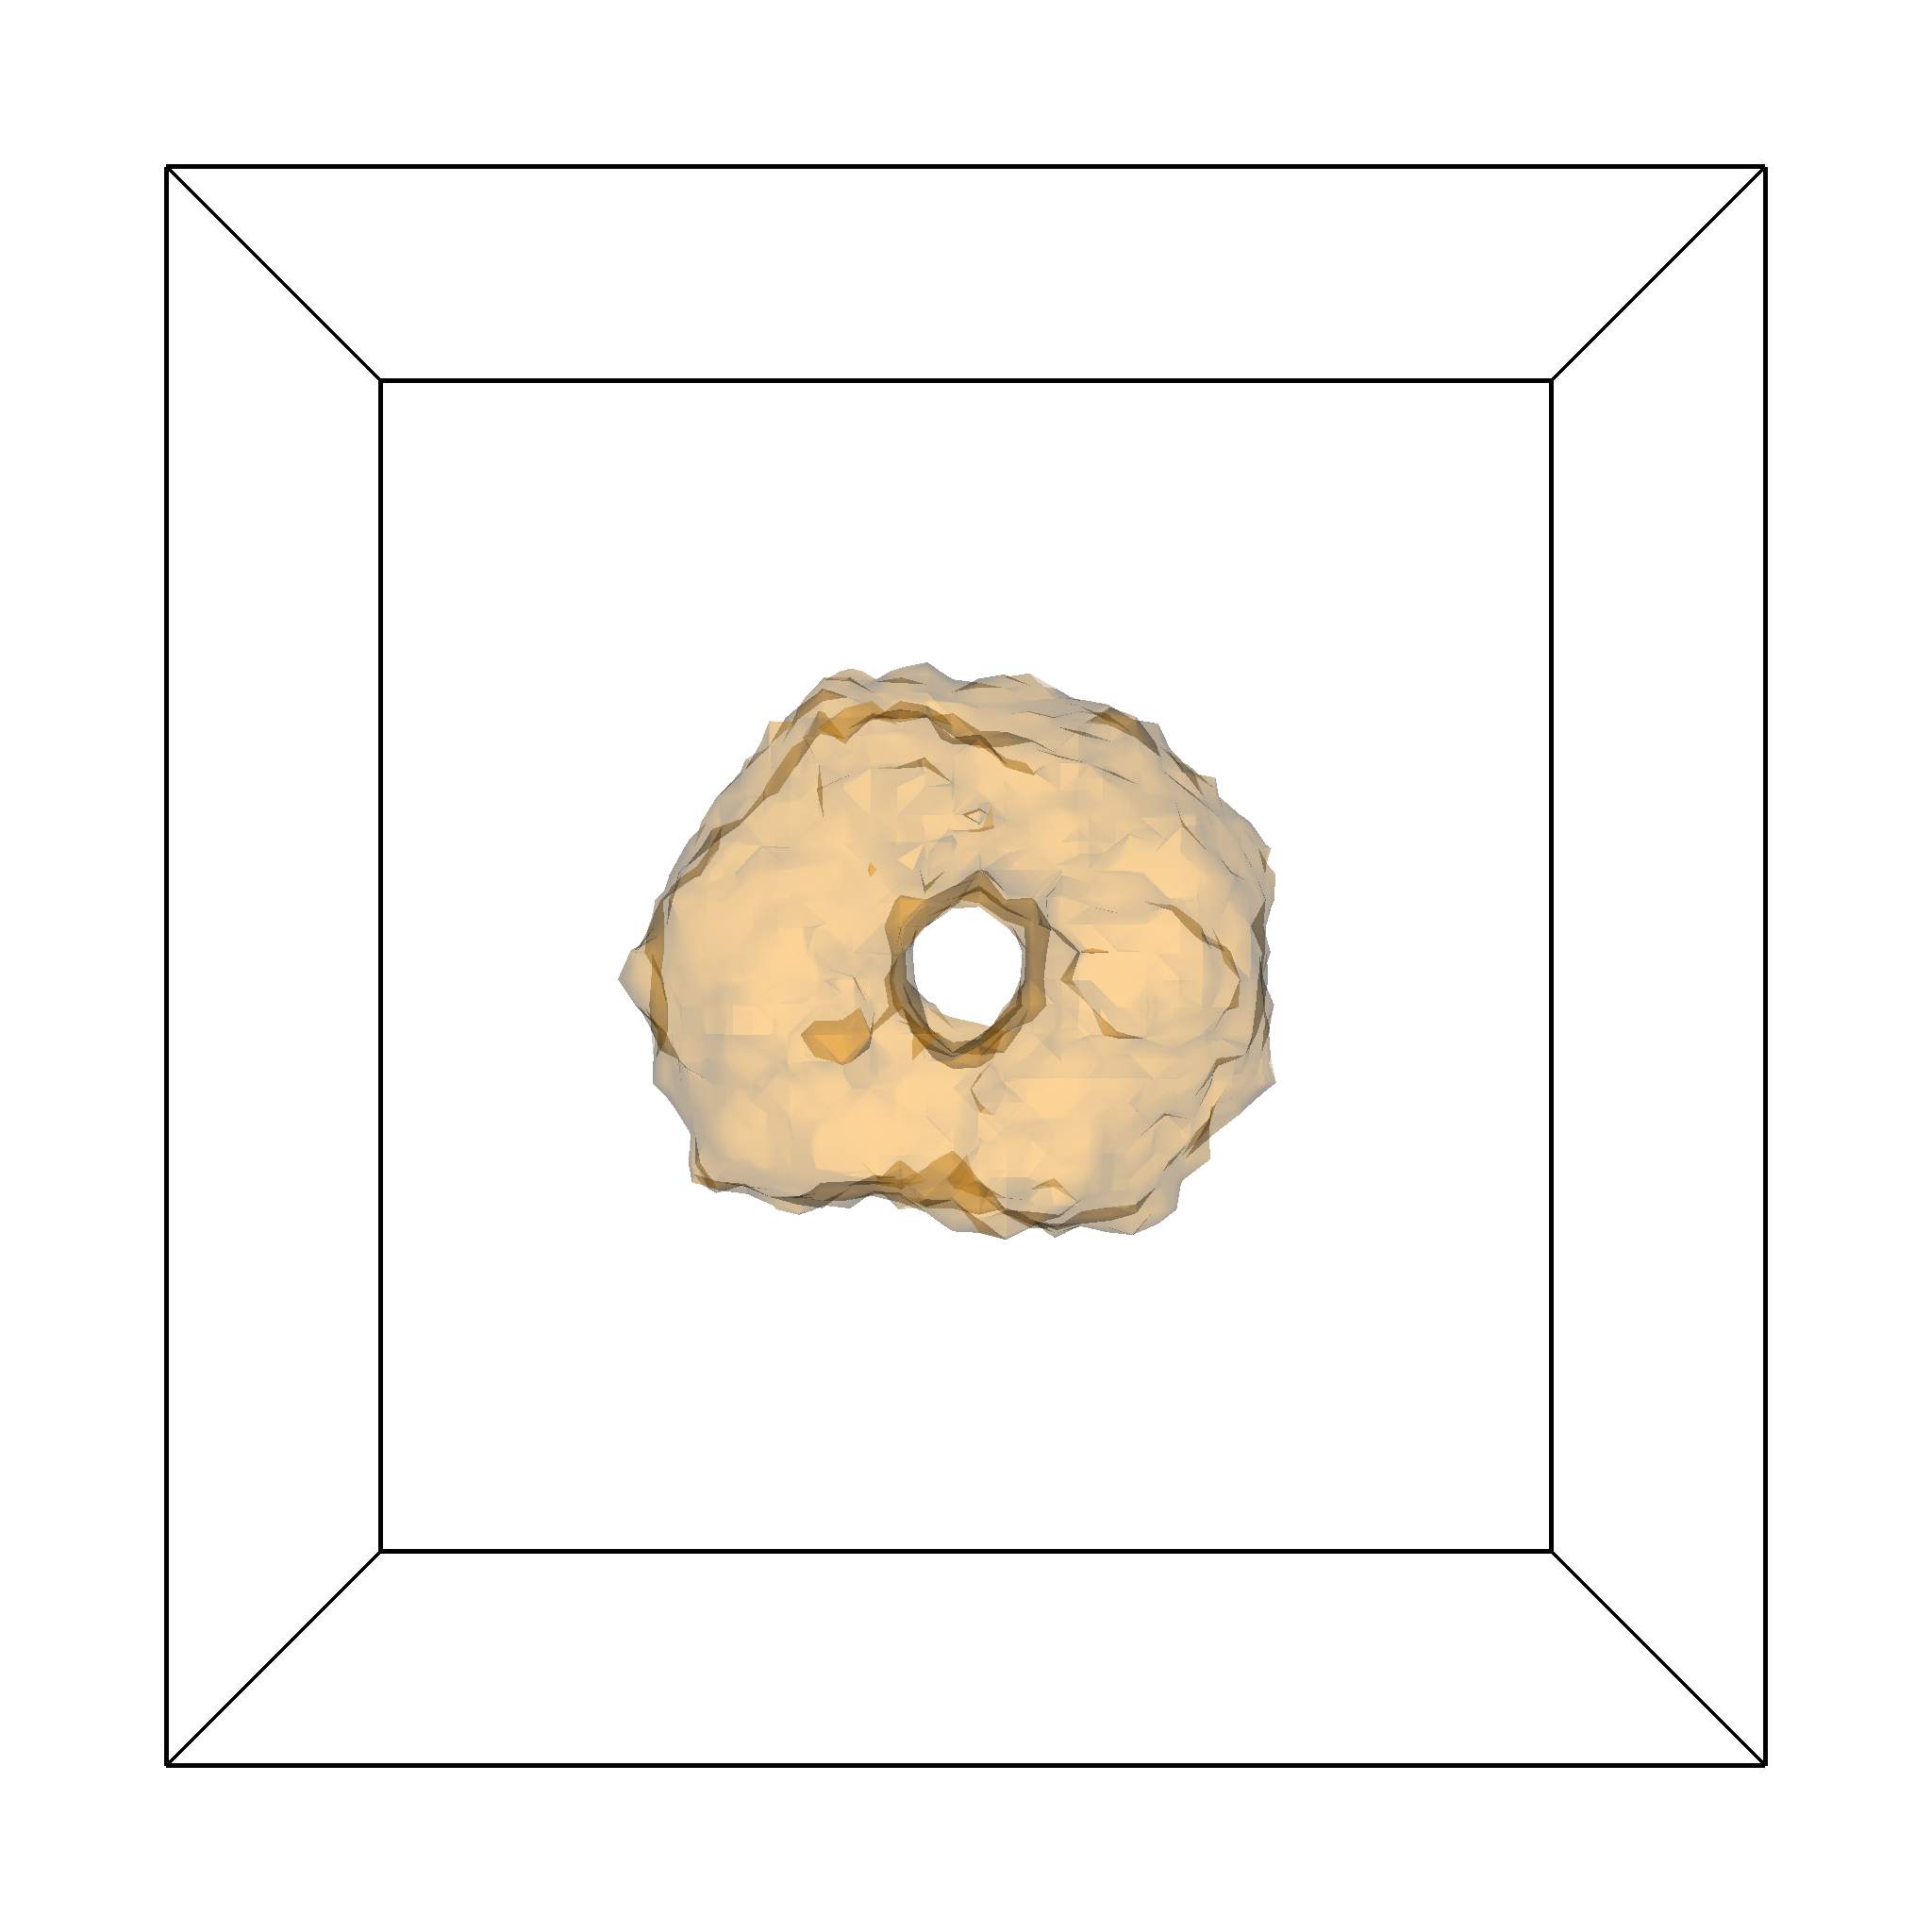
\includegraphics[width=0.165\columnwidth]{DC1_NC2_pt2.png}}
	\subfloat[][]{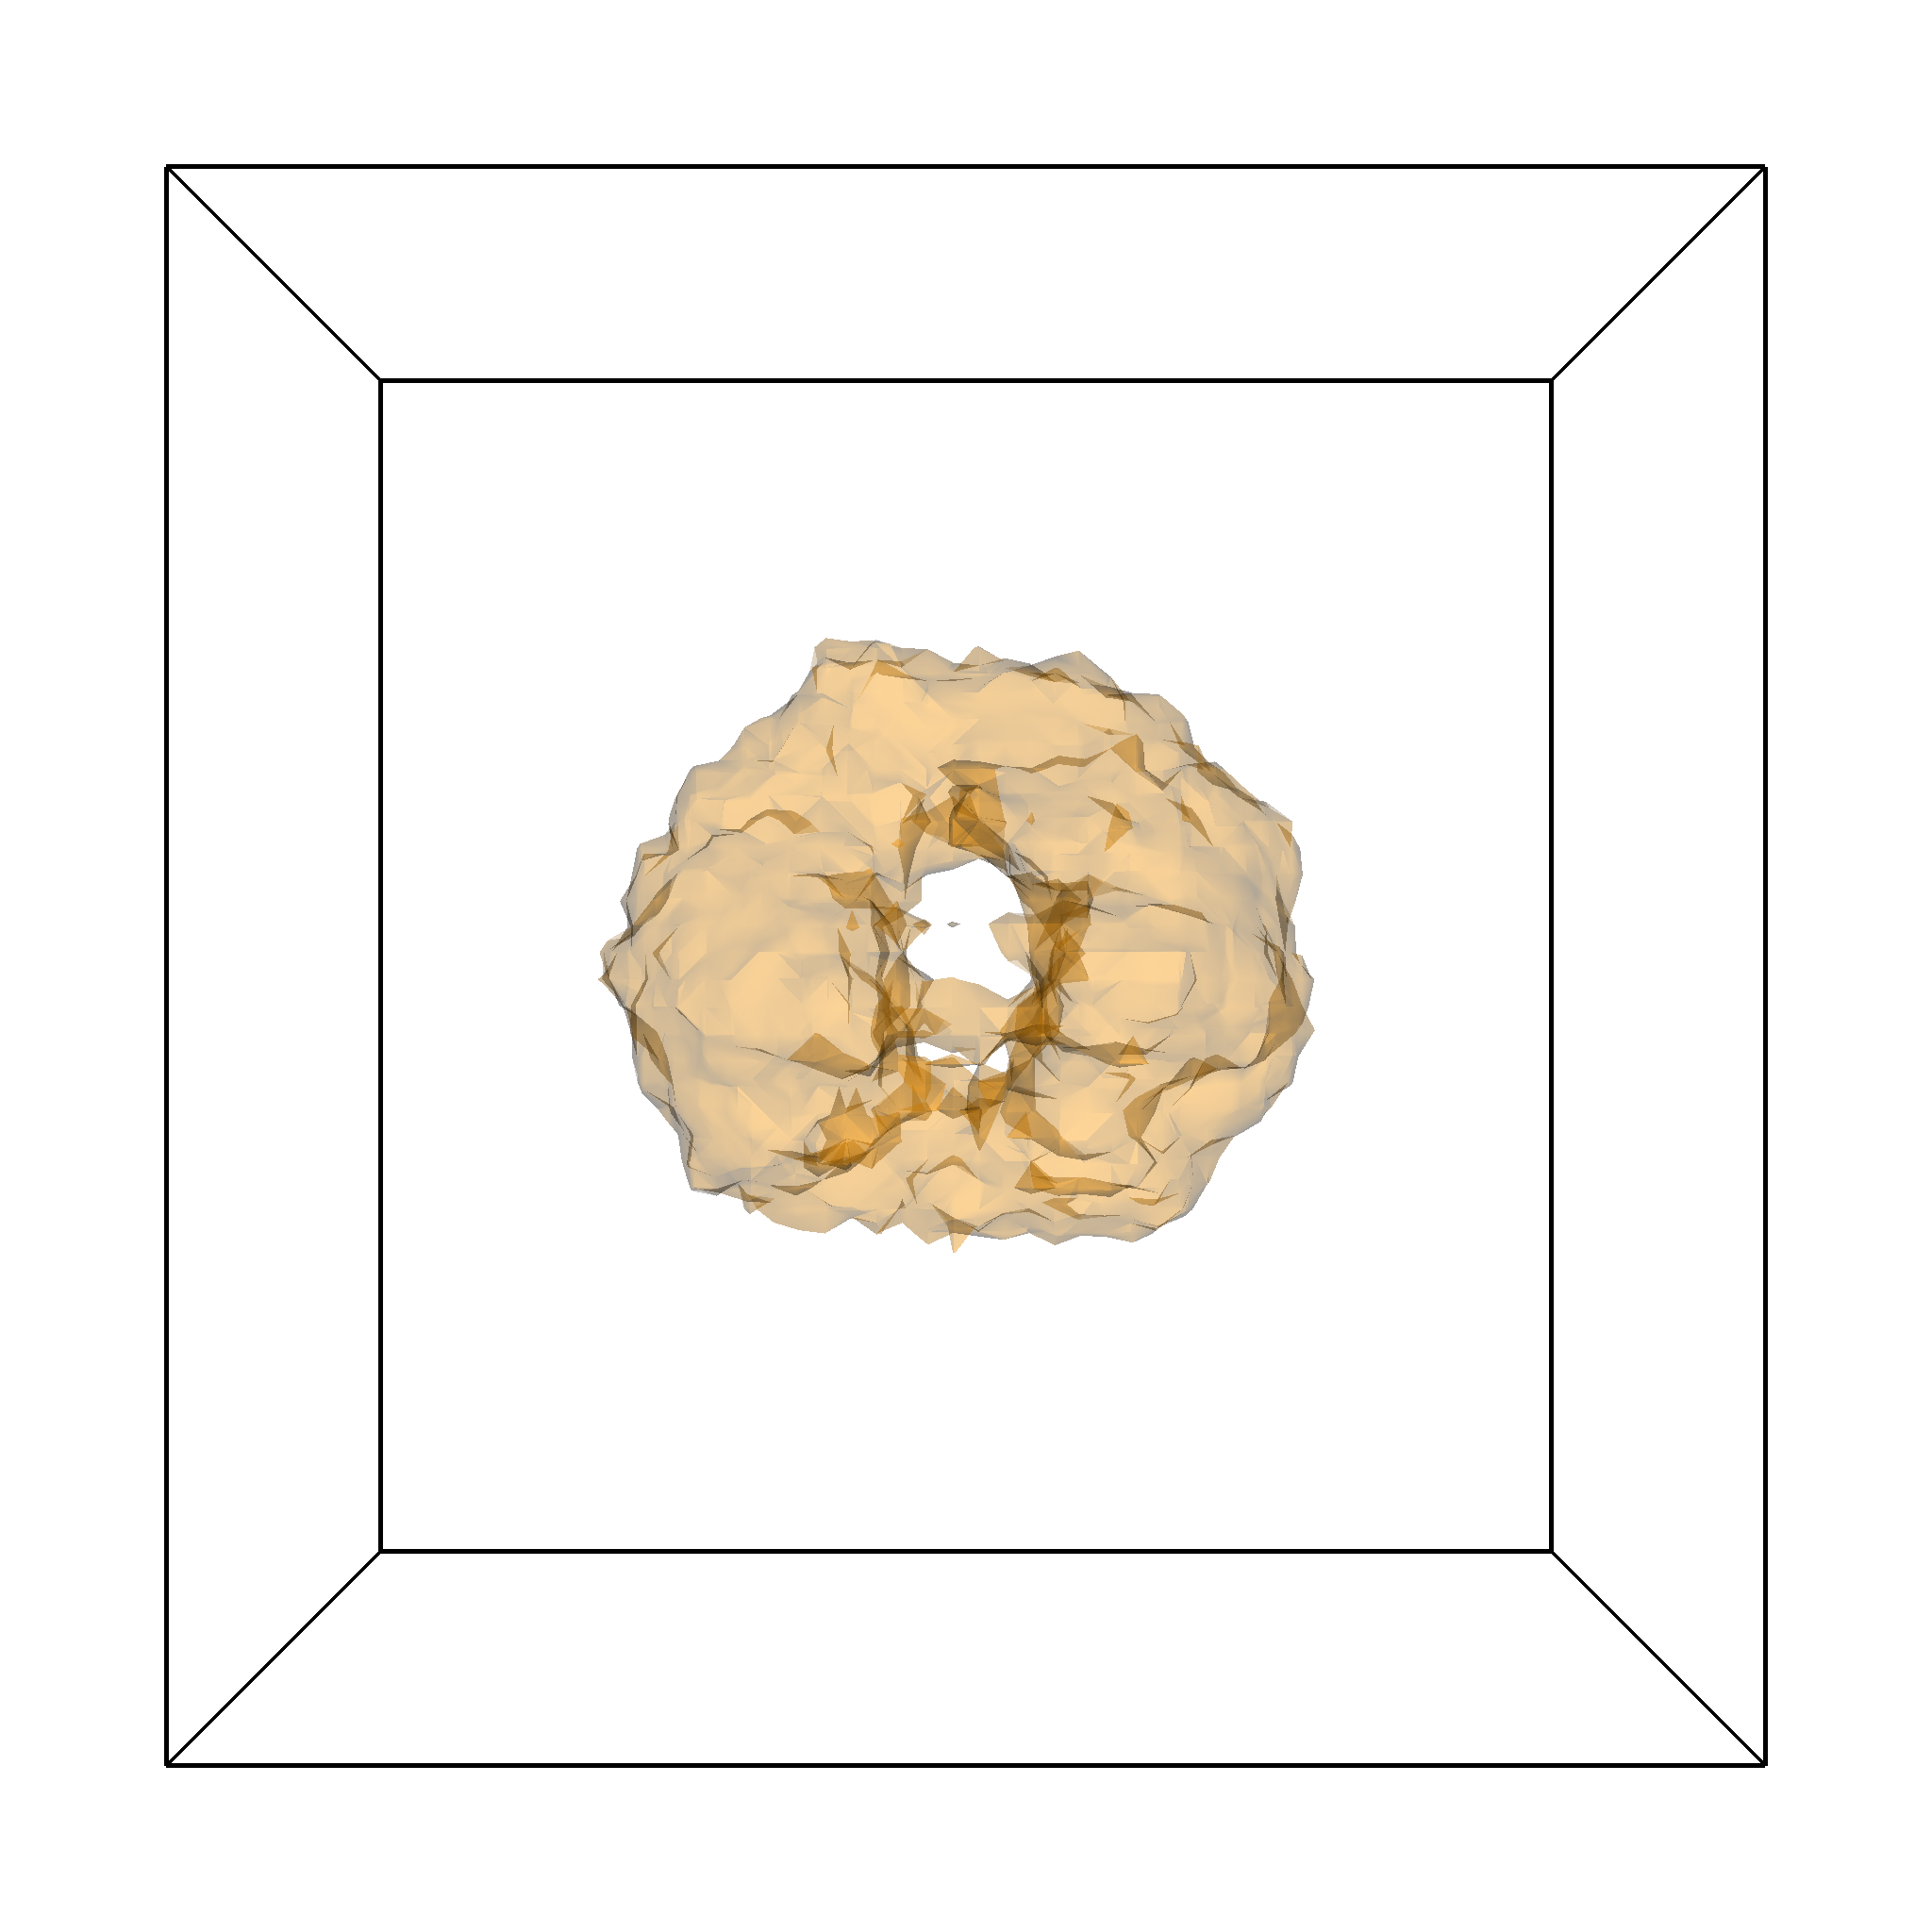
\includegraphics[width=0.165\columnwidth]{DC1_NC2_pt4.png}}
	\subfloat[][]{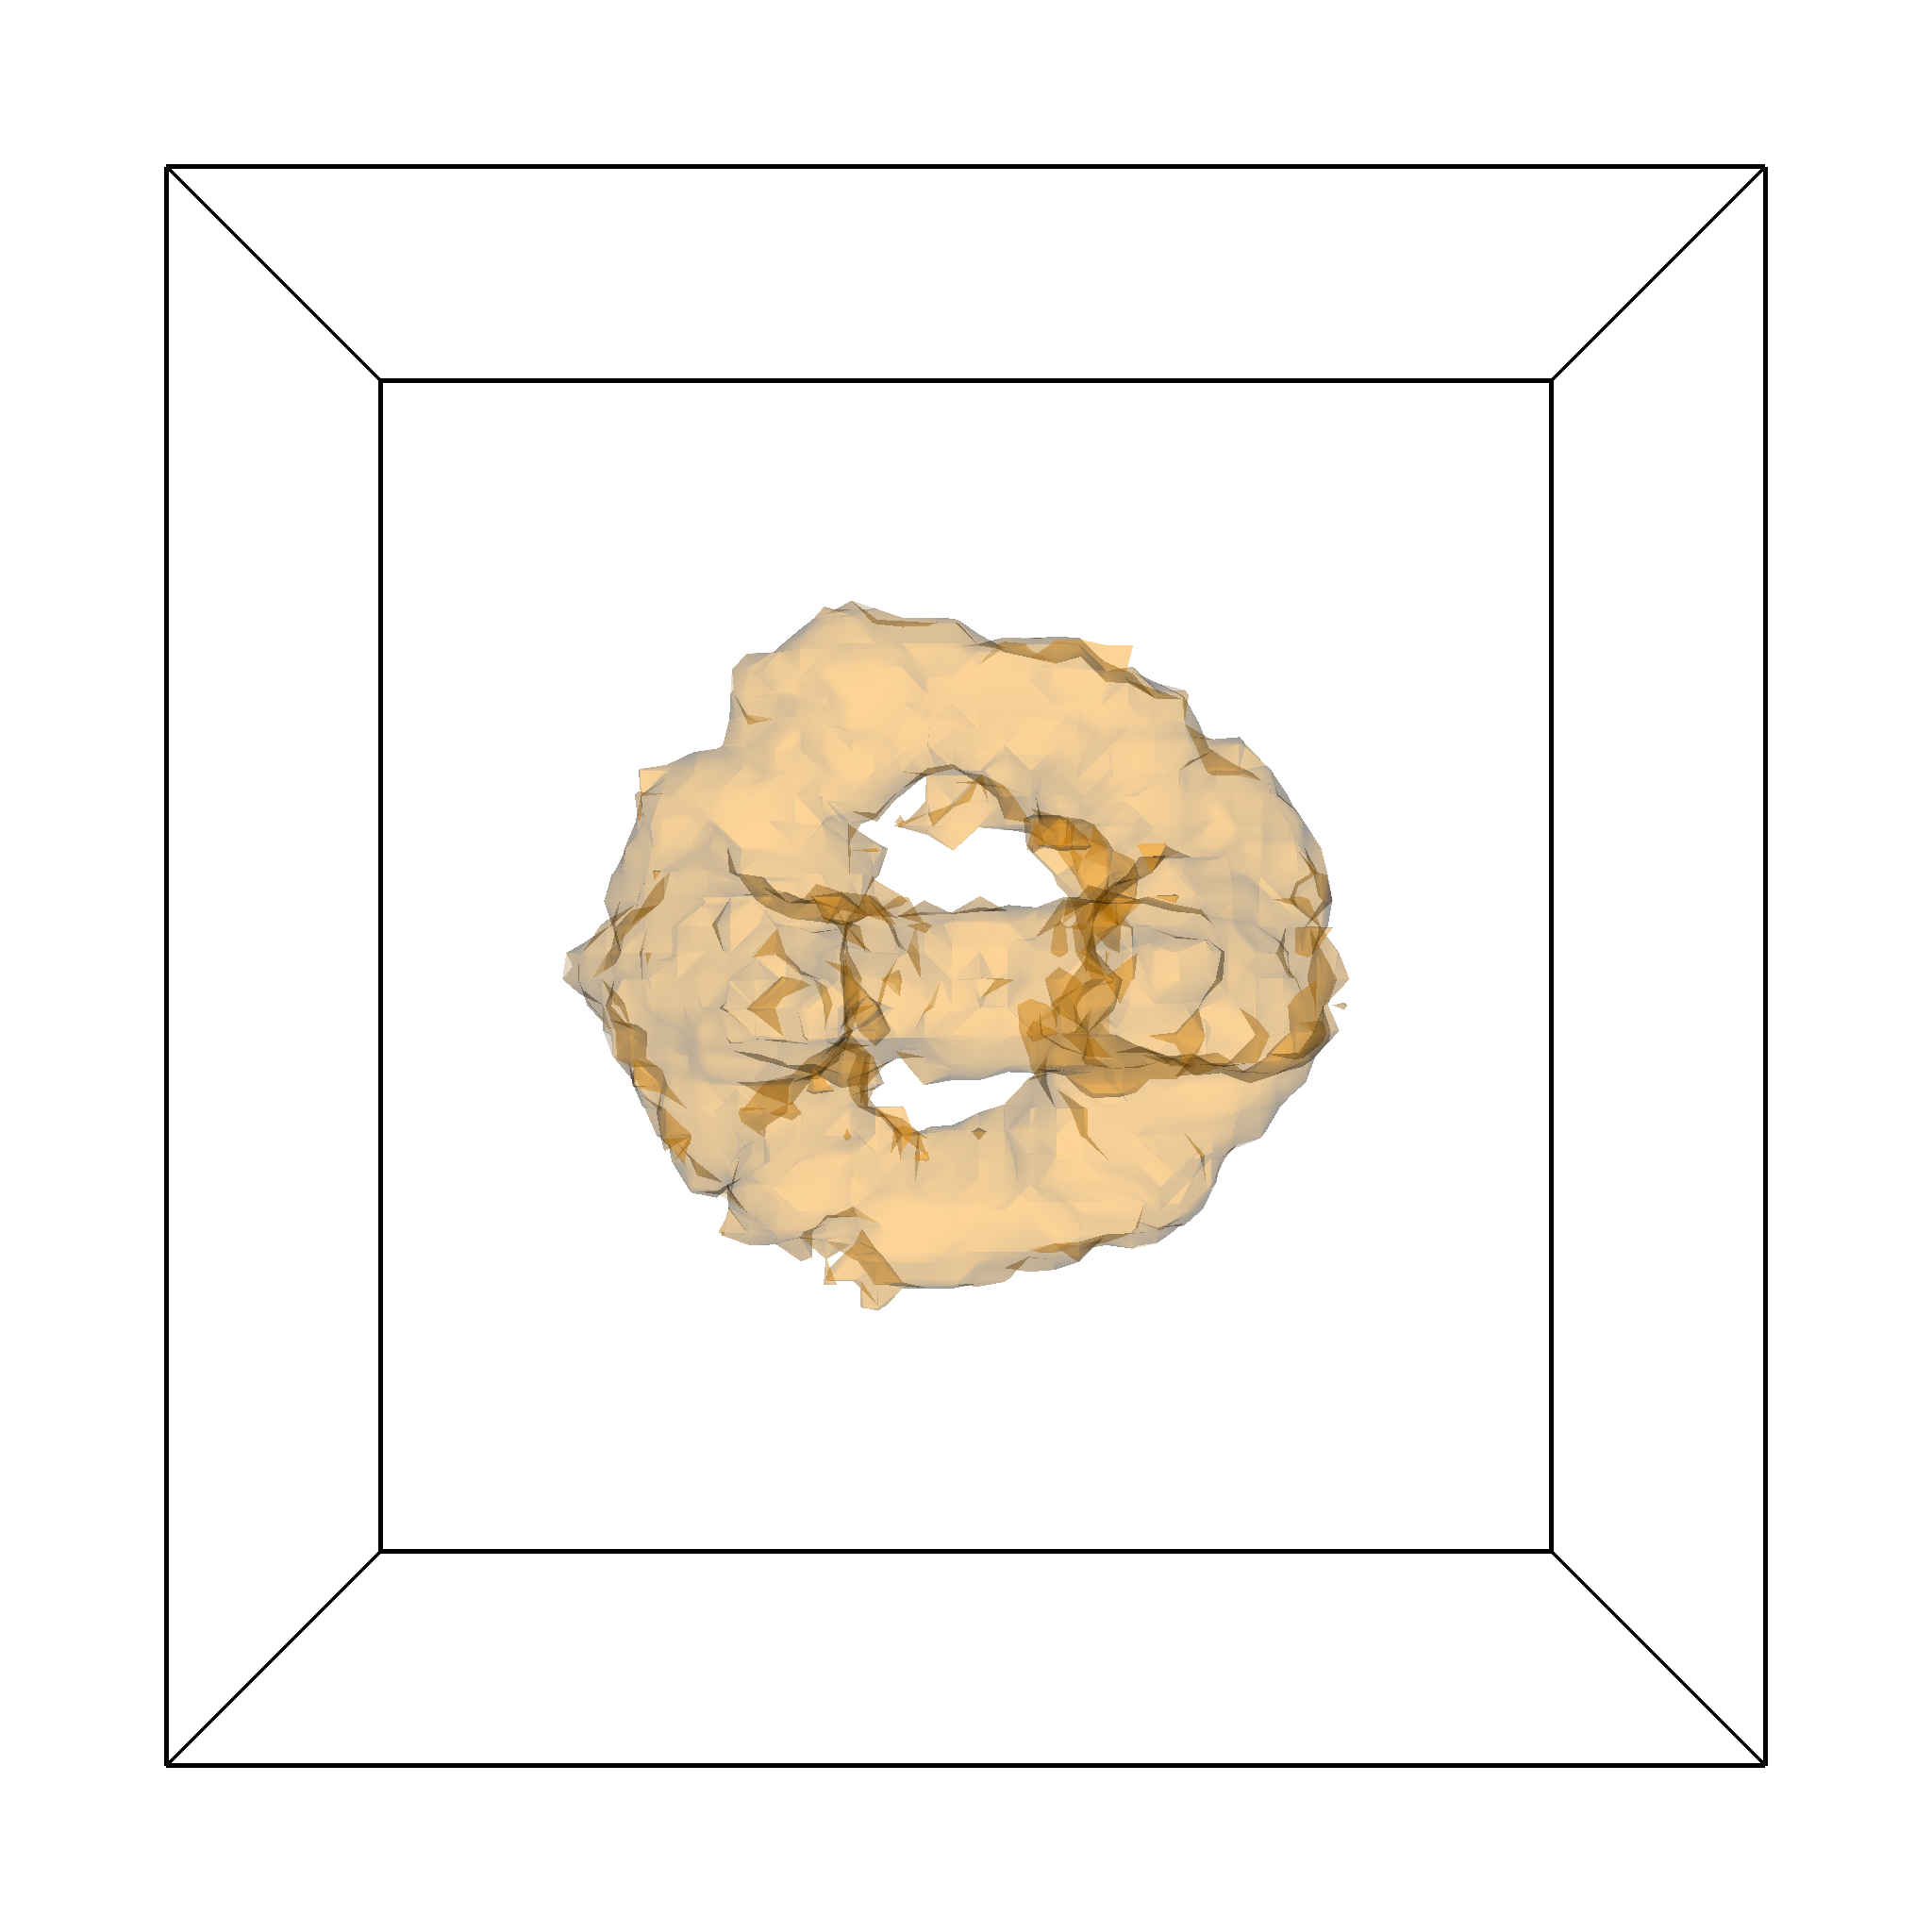
\includegraphics[width=0.165\columnwidth]{DC1_NC2_pt6.png}}
	\subfloat[][]{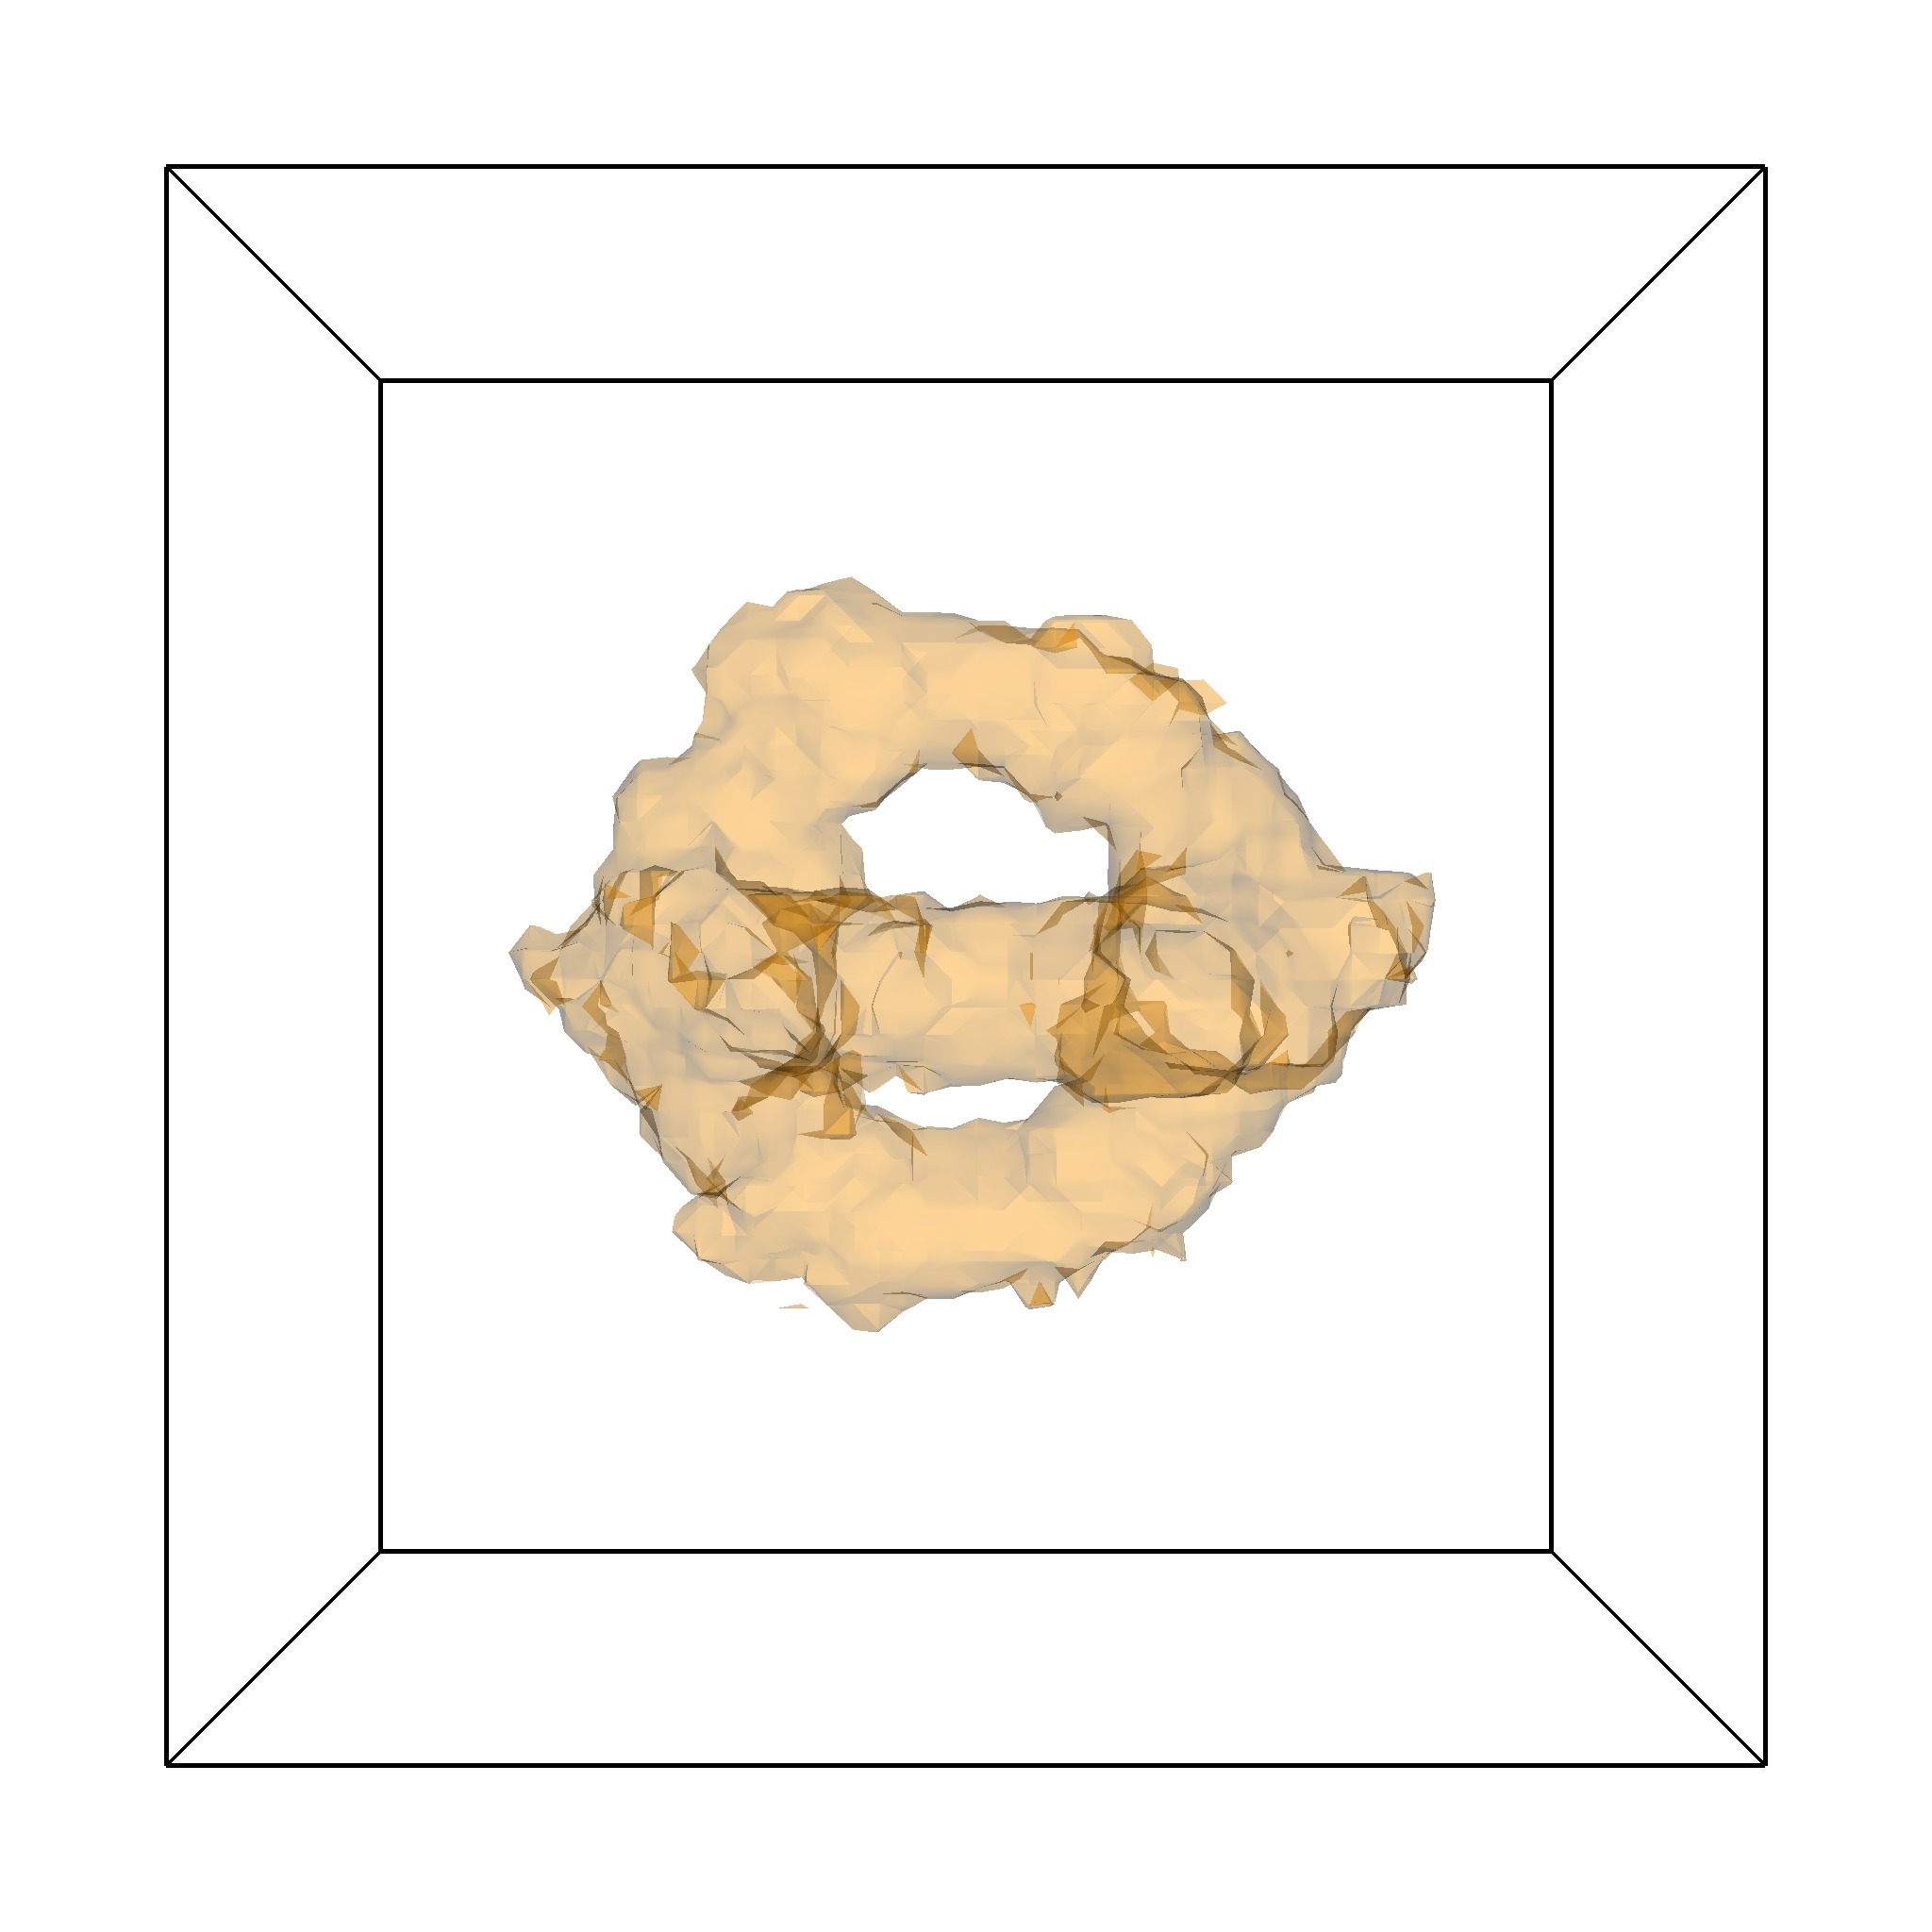
\includegraphics[width=0.165\columnwidth]{DC1_NC2_pt8.png}}
	\subfloat[][\textbf{DC1}]{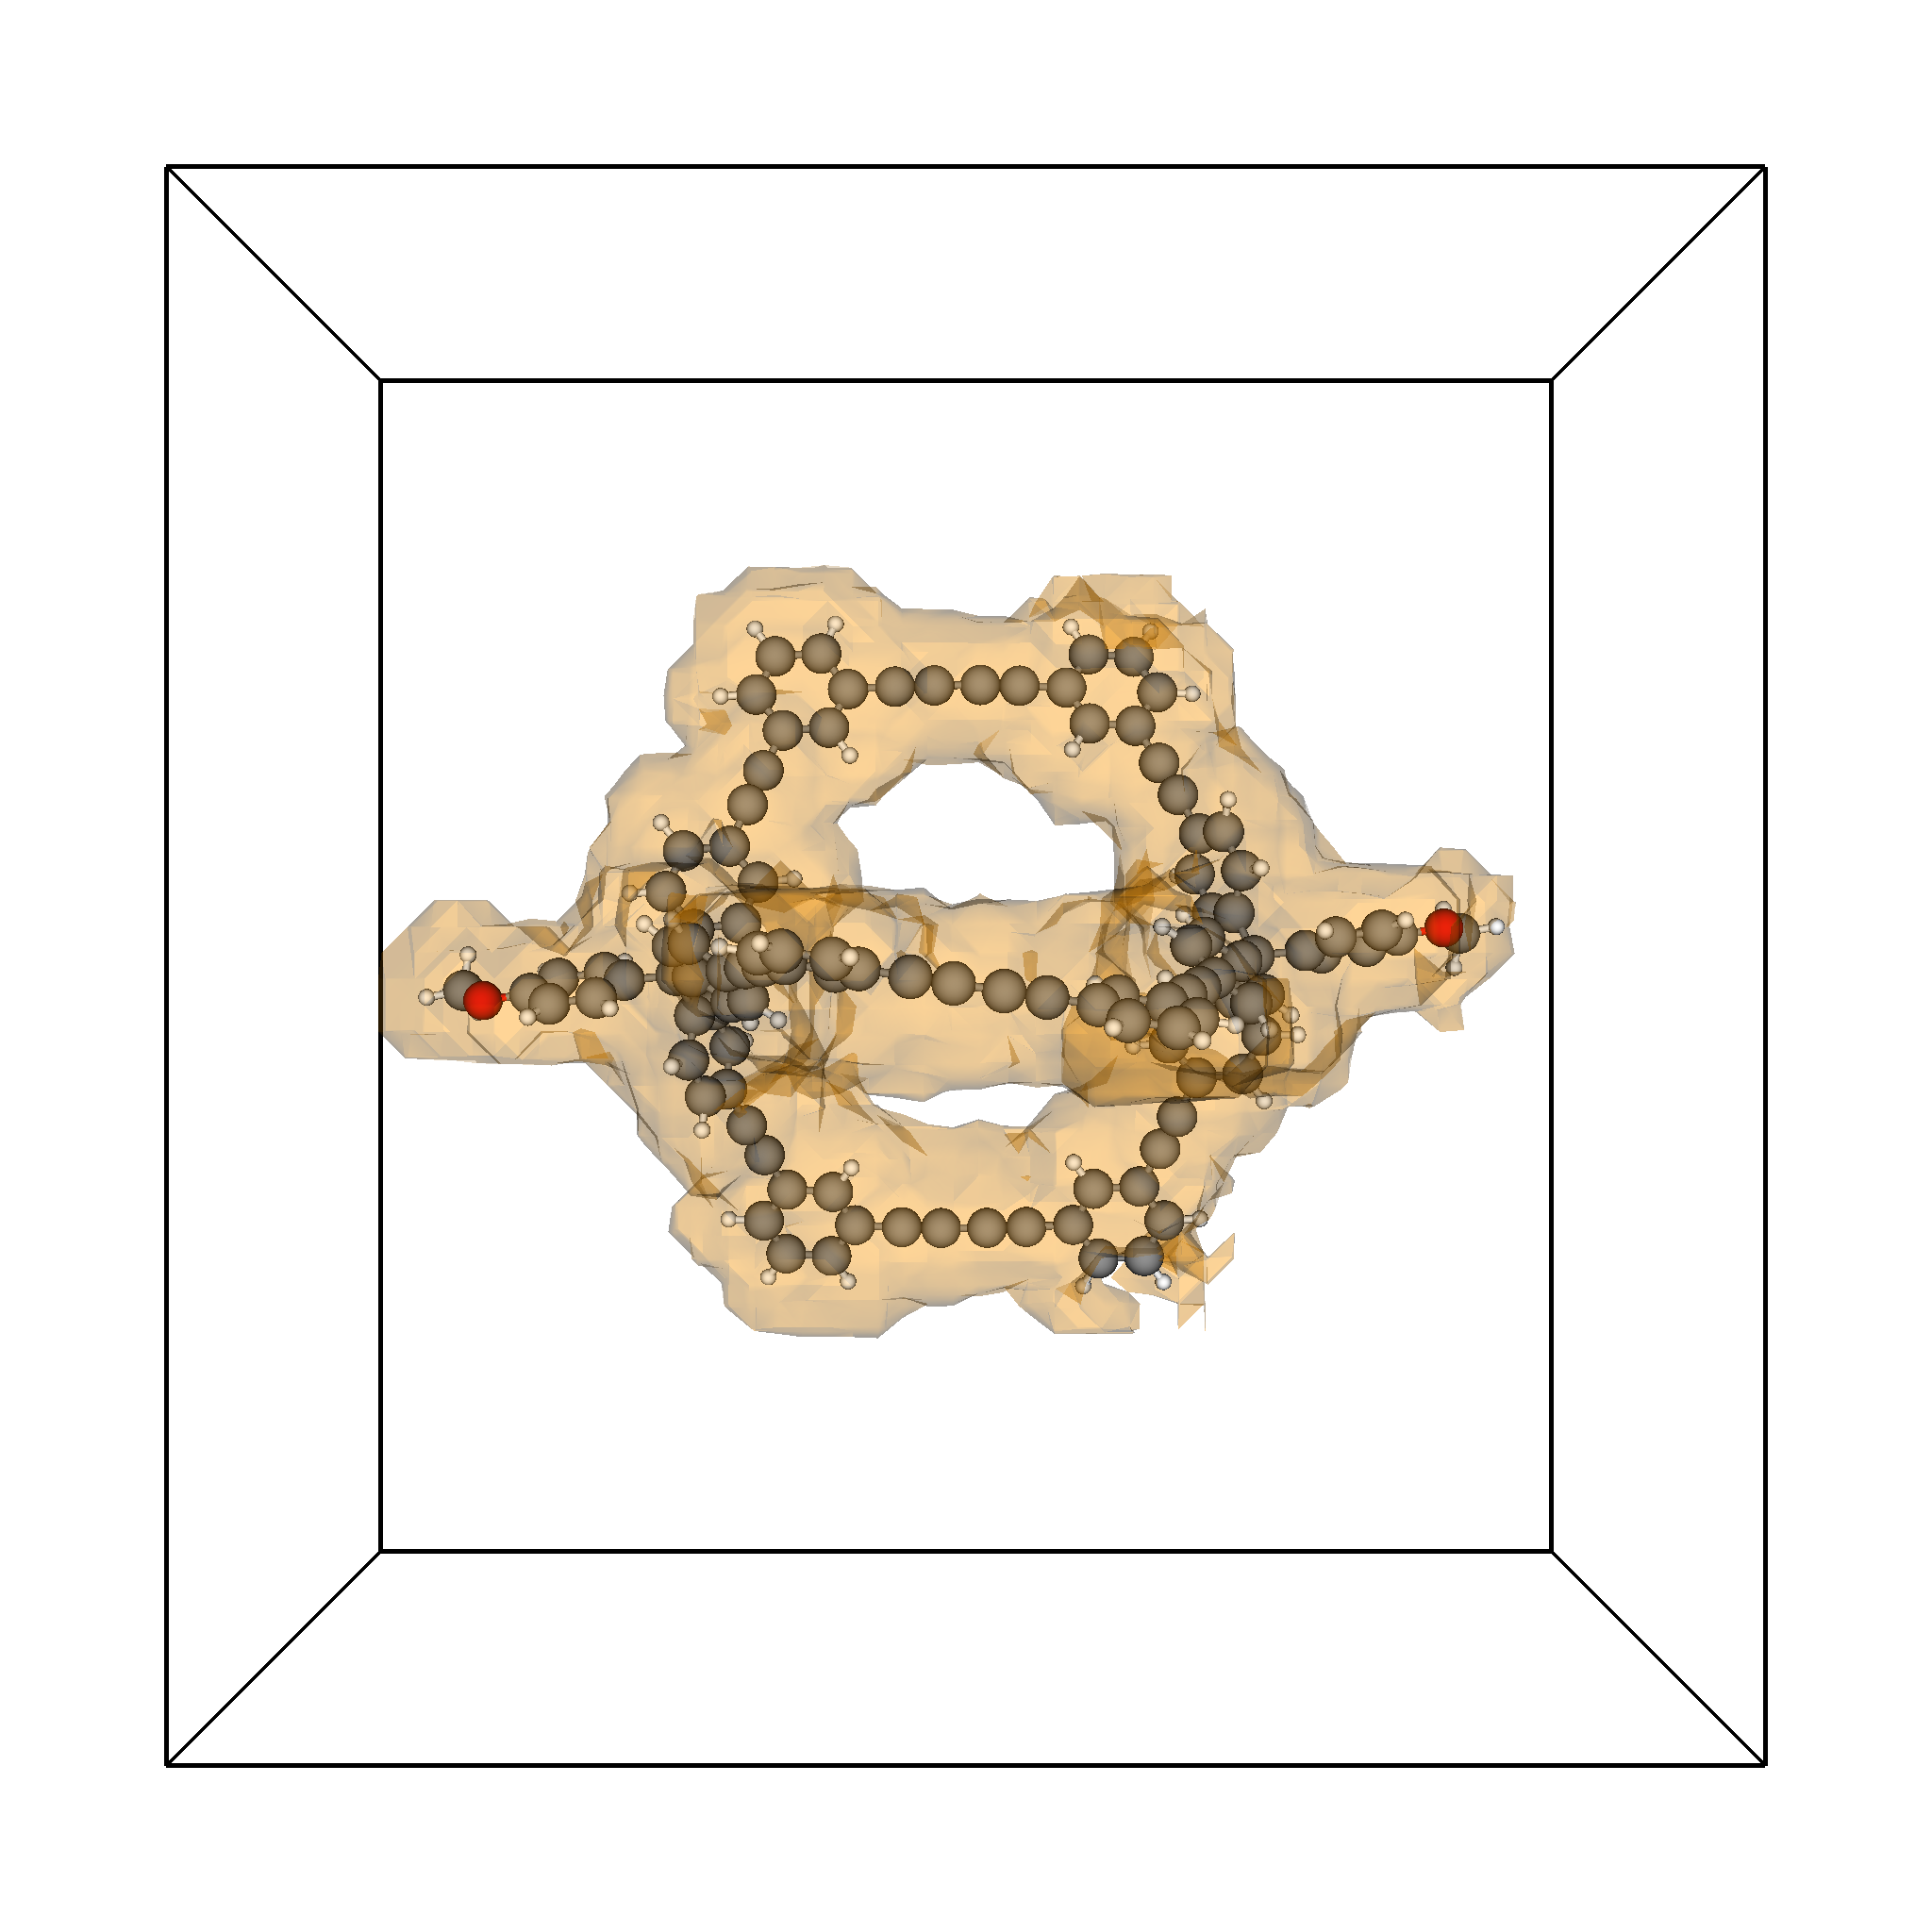
\includegraphics[width=0.165\columnwidth]{DC1_latent.png}}
		\caption{Walking through latent space from cage \textbf{NC2} (a) to \textbf{DC1} (f). (b-e) are fictitious cage cavities generated by walking along a line between the latent representation of \textbf{NC2} and \textbf{DC1}.
	} \label{fig:walk_in_latent_space}
\end{figure}

\subsection{\color{red} Flexible cages occupy a region of latent space}
\label{sec:flexible_MD}
{\color{red}Thus far, we viewed the cage molecules as rigid. But, often cages are flexible to some degree \cite{chen2014separation,camp2016transition,holden2014gas,holden2016understanding}, and the shape of their cavity fluctuates \cite{chen2014separation}, which influences adsorption \cite{witman2017influence}.
To explore the effects of flexibility/ structural fluctuations of cages on their latent representations, we performed molecular dynamics (MD) simulations in the NVT ensemble ($T=298$ K) on four empty, isolated cages (\textbf{CC2}, \textbf{CC3}, \textbf{CC4} and \textbf{CC5}) using a polymer specific consistent force field (PCFF) \cite{sun1994ab,sun1994force,sun1995ab} as implemented by \texttt{DL\_FIELD v4.3} \cite{Yong2016dlfield} and a cage specific force field (CSFF)\cite{holden2012bespoke}. See Sec.~\ref{sec:flexibility} for details. We gathered snapshots of each cage while they were fluctuating in the MD simulation, computed their 3D porosity images, then projected them onto a $\nu=2$-dimensional latent space. Fig.~\ref{fig:pca_space_with_flex} shows that flexible cages, on the basis of the MD snapshots, each occupy a \emph{region} in latent space. The size of the region is determined by the degree of flexibility of the cage; for example, the larger cage \textbf{CC5} explores a larger region of latent space than \textbf{CC3}. Moreover, the latent regions may overlap (as the case with \textbf{CC3} and \textbf{CC4}), indicating that, a fraction of the time, the cages exhibit a very similar cavity shape. 
Analyzing the region in latent space explored by flexible cages could provide more information about fluctuations of cavity shape than simple descriptors such as pore diameter since our latent representation can capture more complex features. Still, considering a rigid cage-- the average configuration of a cage-- is valuable while requiring significantly less computational expense.
}


\section{Conclusions and Discussion}
The idea to exploit different affinities of gases for a surface to purify a gaseous mixture is more than one hundred years old \cite{boyle1908theabsorption}. Since, advanced classes of materials harboring nano-sized pores such as porous cage solids \cite{hasell2016porous,holst2010porous} have emerged and offer high adsorptive selectivities \cite{mastalerz2011salicylbisimine,tian2009amorphous,
hong2015porphyrin,chen2014separation,patil2016noria,sf6seps}.
%Since, nanoporous materials such as zeolites \cite{davis1991zeolites}, metal-organic frameworks \cite{furukawa2013chemistry}, covalent organic frameworks \cite{diercks2017atom}, and porous polymer networks \cite{lu2010porous} offer large surface areas and tunable pore geometries and surface chemistries to enable energy-efficient, adsorption-based gas separations in several arenas \cite{herm2013hydrocarbon,banerjee2014potential,
%sumida2011carbon,li2011metal}. 
Because the size and shape of the cavity intrinsic to a porous organic cage molecule can strongly influence selectivity for its deployment in a molecular separation or sensing application\cite{mitra2013molecular}, it is important to mathematically characterize the void spaces of porous organic cage molecules for predicting adsorption and comparing materials. 

In this study, we computationally scanned the {\color{red} porosity} of 74 porous organic cage molecules to generate three-dimensional images, {\color{red} with the cavity in the center of the image}. The flattened image serves as a raw vector representation of the intrinsic porosity of a cage that lies in a very high-dimensional space. We postulated that the 3D porosity images effectively lie in a much lower dimensional subspace of this enormous space. Using the singular value decomposition, we learned in an unsupervised manner the effective lower-dimensional subspace in which the void spaces of porous organic cages sit, which is characterized by a set of \emph{eigencages}. Expressing a cage as a linear combination of eigencages defined its \emph{latent representation}, which lent a notion of similarity between two cages. We embedded the latent representations of the porous organic cage molecules into two-dimensional space to visualize the clusters of cages. We found that the clusters in the learned latent space coincide with our intuition of cages exhibiting similarly-shaped cavities and that cages can be visually reconstructed from their low-dimensional latent representation. Furthermore, cages nearby in latent space are more likely to exhibit similar simulated Xe/Kr selectivities, cavity diameters, and number of windows entering the cavity. Together, this shows that our $\nu=22$-dimensional latent representation efficiently encodes the salient features of the cavities in the porous cages displayed in Fig.~\ref{fig:cages}.

We host an interactive visualization of the latent cage space at \url{simonensemble.github.io/latent-cage-space}. If a given cage exhibits a high adsorptive selectivity for a gas separation or sensing application as a consequence of its cavity shape, one can search nearby in latent cage space for likely similar performers.

%An interesting question is: what is the effective dimensionality of intrinsic void spaces displayed by the set of porous cage molecules synthesized to date? 
The degree of compression of the 74 3D porosity images by the singular value decomposition sheds some light on the diversity of cages that have been synthesized. A $\nu=22$ dimensional latent representation-- a 70\% compression of the 3D porosity images-- incurred less than 15\% relative error. Consequently, one might suggest that the cavities of the 74 cages in Fig.~\ref{fig:cages} are composed of approximately 20 orthogonal cavity ``motifs'' (eigencages). As only 12 of the at least 20 probable porous organic cage molecule topologies have been synthesized \cite{santolini2017topological}, our latent space representation will be useful in comparing and predicting the properties of the many porous organic cage molecules that are likely to emerge in the future.

At this juncture, we mention the limitations of this work. First, often cages are found to be flexible \cite{chen2014separation,camp2016transition,holden2014gas,holden2016understanding} as opposed to rigid as we took the cages here. {\color{red} In reality, we showed that cages occupy a region in latent space, not a point.} Second, as we considered only a single cage molecule in isolation, the latent cage space includes only the notion of intrinsic void space, as opposed to the extrinsic void space that can arise from how the cages pack together to form the bulk solid \cite{hasell2016porous}. In fact, assembly of porous cage molecules to form a bulk solid can be sensitive to small changes in the cage molecule \cite{hasell2014controlling}. Depending on the outer surface chemistry and geometry of the molecule, the assembly/packing of porous organic cage molecules can be such that the intrinsic pores in the bulk solid are isolated!\cite{tozawa2009porous} {\color{red} For this reason, the simulated Xe/Kr selectivities in the isolated cage molecules in Fig.~\ref{fig:latent_space_S_Xe_Kr} may not necessarily be a quality prediction of the selectivity in the bulk cage solid. Our analysis of potential energies of adsorption sites in/on the cage molecules in Fig.~\ref{fig:energy_vs_dist}, however, suggests that the dominant adsorption site in cages exhibiting the highest simulated Xe/Kr selectivity tend to be internal to their cavity; hence false positives may be unlikely unless the internal sites are blocked. See Sec.~\ref{sec:kh_isolated} for more discussion.} A third limitation is that, while we may aim for the singular value decomposition to learn distinguishing features of the \emph{cavities} of the cages\footnote{\color{red} We did our best to encourage SVD to focus on the cavity by (i) centering the cavity in the image and (ii) aligning cages based on the porosity point cloud tracing out the shape of the inner-cavity.}, the algorithm takes notice of the moieties protruding from the core in addition to the internal cavity. {\color{red} This is evident by e.g. the distance between \textbf{C9} and \textbf{C1} and \textbf{RCC1a} and \textbf{RCC1c} in Fig.~\ref{fig:latent_space}.} A method to incentivize a dimensionality reduction algorithm to pay more attention to the center of the cage may be warranted if the internal cavity is the most important feature to describe. That said, the encoding of the periphery of the molecule may be desirable for e.g. predicting how cage molecules assemble to form the solid. The final limitation is that the singular value decomposition is sensitive to alignments and translations for inter-cage comparisons. {\color{red} One's mathematical definition of ``optimal alignment'' (e.g.\ using rotational dynamics or Coherent Point Drift) may not coincide with one's intuition of how the cages should be aligned. Our future work is to employ rotational-invariant algorithms that detect features of cavities regardless of their orientation.}

{\color{red} When computationally scanning the cage molecule to generate the 3D porosity image, we binarized each pixel as void space or overlapping the cage structure using helium as a probe. This ensures that the 3D porosity image only contains information about the shape of the cage molecule and its cavity. Another option to likely lend a more predictive feature for a regression model of adsorption of a particular gas is to instead assign the pixel value to be the free energy of adsorption of that gas centered at that point. For this study, we elected to binarize the pixels to yield a more generalizable latent representation and avoid overfitting the latent representation to describe a particular gas.}

{\color{red} One may question why we do not employ t-SNE \cite{maaten2008visualizing} directly to reduce the dimensionality of the 3D porosity images. The inventors of t-SNE themselves first used principal component analysis (directly related to SVD) to reduce the dimensionality of images of handwritten digits preceding t-SNE to filter out noise and to speed up the computation \cite{maaten2008visualizing}. Our reasons for employing SVD instead of t-SNE directly are (i) the mapping by SVD lends more interpretability through visualizing the eigencages (Fig.~\ref{fig:eigencages}), (ii) unlike t-SNE, SVD provides an explicit mapping function that can be used to (a) project unseen data into the latent space as we did with our MD snapshots and (b) generate fictitious pore structures as we did between \textbf{NC2} and \textbf{DC1} (iii) t-SNE is stochastic, whereas SVD is deterministic. 
}

To further the ideas in this study, we are working towards embedding the pore structures of extended network materials such as metal-organic frameworks (MOFs) into a low-dimensional latent space. MOFs are more tunable materials than porous cages, as exemplified by the tens of thousands of MOFs that have been reported \cite{moghadam2017development} in comparison to the hundreds of porous cage solids \cite{evans2016computational}; thus, MOFs exhibit a greater diversity in their void space architectures. However, MOFs present a more formidable challenge than porous organic cage molecules because their 3D porosity images are periodic with varying Bravais lattices. We are exploring how more advanced dimensionality reduction algorithms such as autoencoders \cite{hinton2006reducing} with convolutional layers \cite{kavukcuoglu2010learning,zeiler2010deconvolutional} may fare at learning/detecting hierarchal features of pore structures with translational and rotational invariance.

\begin{acknowledgement}

% Please use ``The authors thank \ldots'' rather than ``The
% authors would like to thank \ldots''.

C.M.S. and A.S. thank the School of Chemical, Biological, and Environmental Engineering at Oregon State University for start-up funds. M.T.H. thanks the Pete and Rosalie Johnson Internship Program at Oregon State University. A.H.P.Y. thanks the URSA Engage Program at Oregon State University. {\color{red} We thank the anonymous reviewers for helpful comments that led to improvements in our results and the text.}

\end{acknowledgement}

%% Notice that the class file automatically sets \bibliographystyle
%% and also names the section correctly.
%%%%%%%%%%%%%%%%%%%%%%%%%%%%%%%%%%%%%%%%%%%%%%%%%%%%%%%%%%%%%%%%%%%%%


\section{Supplementary Information} A Jupyter Notebook with Julia \cite{julia} code to reproduce the data in this article is available on Github at \url{github.com/SimonEnsemble/latent_cage_space}; the 3D porosity images and Henry coefficients were calculated with our open source code \texttt{PorousMaterials.jl} v0.1.3 \cite{PorousMaterialsJL}. A Supporting Information document is also available.

\bibliography{bibfile}
\end{document}
